\clearpage
\thispagestyle{plain}
\lettrine{F}{rom}~the decay-time spectrum of \BsDsK~events, the \CP-violation parameter~\CPgamma can be measured.
This is done in two steps: first, a statistically clean sample of \BsDsK~candidates is obtained, after which the decay-time distribution of this sample is fitted.
The complete analysis strategy is as follows.\\

\noindent \textbf{\large{\Cref{chp:BsDsK_TD_Data}}}
\vspace{.5ex}\hrule
\begin{enumerate}
    \item A clean sample of \BsDsK~signal candidates is selected, as well as kinematically similar \BsDsPi~candidates, which are used for calibration purposes.
    \item The \BsDsK~candidates are fitted, in order to subtract the background and obtain a statistically clean signal sample.
    \newcounter{enumvalue} \setcounter{enumvalue}{\value{enumi}}
\end{enumerate}

\noindent \textbf{\large{\Cref{chp:BsDsK_TD}}}
\vspace{.5ex}\hrule
\begin{enumerate}
    \setcounter{enumi}{\value{enumvalue}}
    \item Flavour tagging information on the resulting candidates is obtained and calibrated with the self-tagging \BsDsPi~candidates.
    \item The experimental decay-time measurement resolution is calibrated using a sample of prompt \Dsmp~events.
    \item \label{it:BsDsK_TD_Strat-dtfit} The \CP-violation parameters are extracted by fitting the decay time of the \Bs~sample, taking into account the tagging information, resolution, and acceptance corrections.
    \item The CKM~parameter \CPgamma~is determined from these parameters.
\end{enumerate}
%
The parameters extracted in step~\ref{it:BsDsK_TD_Strat-dtfit} are \({\Cpar = \Cbpar}\), \Spar, \Sbpar, \Dpar, and~\Dbpar, where~\({f = \DsmKp}\) (see \cref{sec:CPV}).

\clearpage

\setchapterpreamble{
    \lettrine{T}{his}~\lcnamecref{chp:BsDsK_TD_Data} discusses how a statistically pure sample of \BsDsK~candidates is obtained.
    In \cref{chp:DsK_BF}, a similar selection was discussed, which was aimed at obtaining the highest precision in yield and efficiency.
    Here, the selection is instead optimised to obtain for high signal purity, by suppressing as much background as possible.}
\chapter{\BsDsK~signal extraction}
\label{chp:BsDsK_TD_Data}

\vspace*{\fill}
\minitoc

\clearpage
\section{Data and selection}
\label{sec:BsDsK_TD_Selection}

\subsection{Data sample}
The data sample used for the analysis corresponds to an integrated luminosity of~\SI{3.0}{\per\femto\barn} of \({\proton\proton}\)-collision data recorded with the \lhcb~detector, of which \SI{1.0}{\per\femto\barn}~(\SI{2.0}{\per\femto\barn}) at \({\sqs = \SI{7}{\TeV}}\)~(\SI{8}{\TeV}).
About half of this data is taken with the opposite polarity of the \lhcb~magnet.
The preselection outlined in \cref{sec:stripping} is applied to this sample.
Candidates are reconstructed with the following final states\footnote{
    Charge conjugation is implied throughout this \lcnamecref{sec:BsDsK_TD_Selection}.}
(hereafter referred to as ``modes''):
%
\medskip
\begin{center}
\begin{tabular}{llp{5cm}}
    \toprule
    \BsDsK,  & \DsmKKPi   & The main signal channel;\tabularnewline[1ex]
    \BsDsK,  & \DsmPiPiPi & \multirow[t]{2}{=}{The \Dsm~branching fractions of these channels are lower, but they add to the statistics of the signal sample;} \tabularnewline
    \BsDsK,  & \DsmKPiPi  & \tabularnewline
    \tabularnewline
    \tabularnewline
    \midrule
    \BsDsPi, & \DsmKKPi   & \multirow[t]{3}{=}{This calibration channel is kinematically very similar to~\BsDsK, and has comparatively large statistics;} \tabularnewline
    \BsDsPi, & \DsmPiPiPi & \tabularnewline
    \BsDsPi, & \DsmKPiPi  & \tabularnewline
    \tabularnewline
    \midrule
    \BdDPi,  & \DmKPiPi   & This highly pure background channel is used to calibrate simulated data to better match the data.\tabularnewline
    \bottomrule
\end{tabular}
\end{center}
\medskip

\subsection{Boosted decision tree}

A~boosted decision tree\footnote{
    The BDT~configuration is defined as \num{300}~trees, each with a maximum depth of two nodes, while requiring that each node contains at least~\SI{4}{\percent} of the input events.
    The variables are scanned at \num{40}~points for the optimal cut value, and events with negative weights are excluded from the sample.}
(BDT, see \cref{sec:MVA}) is used to separate signal from combinatorial background events, which arises from random track combinations that look similar to signal candidates.
The signal input sample used to train this~BDT is chosen to be events of the plentiful decay~\BsDsPi with~\DsmKKPi, selected using the criteria listed in \cref{tab:BsDsK_TD_BDT_selection}.
Note that the companion track is defined as the pion not originating from the \Dsm~candidate (see \cref{sec:stripping}).
The tracks in the sample are refitted with the additional constraint that the \Bs~candidates originate from the closest~PV.
The signal is extracted from a fit to the \DsmPip~mass distribution which consists of a Gaussian shape for the signal and a negative exponential for the background, in which all parameters except the yields have been fixed to values obtained from simulation.
The background is statistically subtracted using the \sfit~method~\cite{Yuehong_sFit} to obtain a (statistically) pure signal sample.
The resulting mass distribution and fit are shown in \cref{fig:BsDsK_TD_BDT_Training_Data}.

As background input sample to train the~BDT, events from data in the upper mass region of the \DsmPip~invariant mass spectrum~(\({\SI[parse-numbers=false]{[5445, 5800]}{\MeVcc}}\)) are used.
Because there is no \Bs~signal in that region, this sample consists purely of combinatorial events, which are the events the~BDT is designed to reject.
Since no PID~information is used as input to the~BDT, the results are also valid for other \Dsm~decay channels with similar decay topology, such as~\DsmKPiPi and~\DsmPiPiPi.
%
\begin{table}[htb] \centerfloat
    \caption{
        \BsDsPi, \DsmKKPi~selection criteria for the sample used in the BDT~training.
        The same selection is applied to the charge-conjugated candidates.}
    \label{tab:BsDsK_TD_BDT_selection}
    \rowcolors{2}{tableshade}{}
    \begin{tabular}{lll}
        \toprule
        Description & Variable & Requirement\tabularnewline
        \midrule
        \DsmPip~mass & \(m(\DsmPip)\) & \(\in \SI[parse-numbers=false]{[5300, 5800]}{\MeVcc}\) \tabularnewline
        Companion~PID & \(\dllkpi(\pim)\) & \(< \num{0}\) \tabularnewline
        \Dsm~candidate mass & \(m(\Dsm)\) & \(\in \SI[parse-numbers=false]{[1940, 1990]}{\MeVcc}\) \tabularnewline
        \Dsm~daughters PID & \(\dllkpi(\Kmp)\) & \(> \num{0}\) \tabularnewline
        \Dm~veto & mass under \pim\Kp\pim hypothesis & \(< \SI{1850}{\MeVcc}\) \tabularnewline
        \hiderowcolors \aligncell{r}{\emph{or}} & \(\dllkpi(\Km)\) & \(> \num{10}\) \tabularnewline
        \showrowcolors\rowcolor{tableshade} \Lcm~veto & mass under \PbarKPi~hypothesis & \(\notin \SI[parse-numbers=false]{[2250, 2320]}{\MeVcc}\) \tabularnewline
        \aligncell{r}{\emph{or}} & \(\dllkp(\Km)\) & \(< \num{5}\) \tabularnewline
        \bottomrule
    \end{tabular}
\end{table}
%
\begin{figure}[tb] \centerfloat
    \hspace*{-1cm}
    \begin{tikzpicture}
        \node[anchor=south west,inner sep=0] (image) at (0,0) {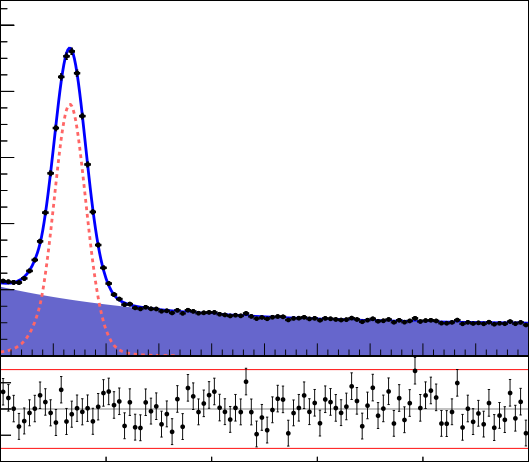
\includegraphics[width=0.9\textwidth]{BsDsK_TD/BDT/BDTG_Training_Bs2Dspi_FullSample_FullMassRange}};
        \begin{scope}[x={(image.south east)},y={(image.north west)}]
            \foreach \x/\xtext in {5300, 5400, ..., 5800}
            {
                \tikzmath{\xpos = (\x - 5300) / 500;}
                \node at (\xpos, -0.025) {\(\xtext\)};
            }
            \foreach \y/\ytext in {0, 2000, ..., 10750}
            {
                \tikzmath{\ypos = ((1 - 0.228) * \y) / 10750 + 0.228;}
                \node[anchor=east] at (0.005, \ypos) {\(\ytext\)};
            }
            \foreach \p/\ptext in {-2, 0, 2}
            {
                \tikzmath{\ypos = ((2 + \p) / 2 + 1) * (0.228 / 4);}
                \node[anchor=east] at (0.005, \ypos) {\(\scriptstyle\ptext\)};
            }
            \node[anchor=east] at (1.0, -0.08) {\({m(\DsmpPipm)}~[\si{\MeVcc}]\)};
            \node[rotate=90,anchor=east,inner xsep=0pt,outer xsep=0pt] at (-0.13, 1.0) {\({\text{Candidates}/(\SI{5}{\MeVcc})}\)};
            \node[anchor=east] at (0.95, 0.90) {\Huge\lhcb};
        \end{scope}
    \end{tikzpicture}
    \caption{
        \DsmpPipm~invariant mass distribution of the data sample used for the BDT~training, with a fit to the data superimposed.
        Note that a small amount of background events remain present in the signal sample, slightly reducing the BDT's~efficacy.}
    \label{fig:BsDsK_TD_BDT_Training_Data}
\end{figure}
%
\begin{figure}[tb] \centerfloat
    \scriptsize
    \begin{subfigure}{.45\textwidth} \centerfloat
        \begin{tikzpicture}
            \node[anchor=south west,inner sep=0] (image) at (0,0) {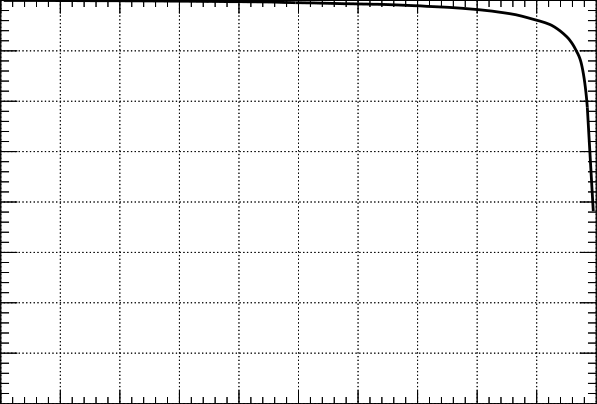
\includegraphics[width=0.9\textwidth]{BsDsK_TD/BDT/BDTG_RocCurve}};
            \begin{scope}[x={(image.south east)},y={(image.north west)}]
                \node at (0, -0.050) {\(0\)};
                \foreach \x in {1, ..., 10}
                    \tikzmath{\xtext = \x/10;}
                    \node at (\x/10., -0.050) {\(\pgfmathprintnumber[fixed,precision=1,fixed zerofill=true]{\xtext}\)};
                \foreach \y in {2, ..., 10}
                    \tikzmath{\ytext = \y/10; \ycoord = (\y - 1.97) / 8.07;}
                    \node[anchor=east] at (0.005, \ycoord) {\(\pgfmathprintnumber[fixed,precision=1,fixed zerofill=true]{\ytext}\)};
                \node[anchor=east] at (1.0, -0.15) {Signal efficiency};
                \node[rotate=90,anchor=east,inner xsep=0pt,outer xsep=0pt] at (-0.14, 1.0) {Background rejection};
            \end{scope}
        \end{tikzpicture}
    \end{subfigure} \qquad%
    \begin{subfigure}{.45\textwidth} \centerfloat
        \begin{tikzpicture}
            \node[anchor=south west,inner sep=0] (image) at (0,0) {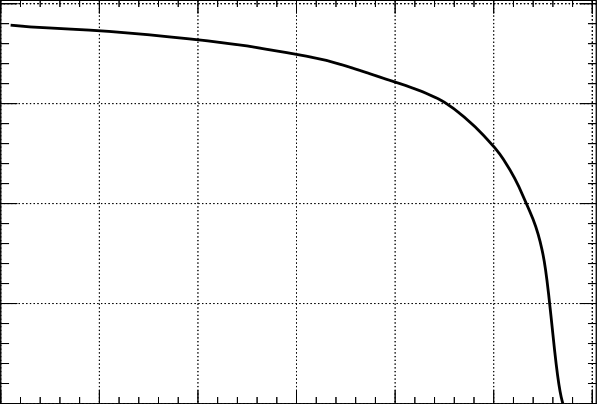
\includegraphics[width=0.9\textwidth]{BsDsK_TD/BDT/BDTG_RocCurve_Zoomed}};
            \begin{scope}[x={(image.south east)},y={(image.north west)}]
                \foreach \x in {7, 7.5, ..., 10}
                    \tikzmath{\xtext = \x/10; \xcoord = (\x - 7) / 3.;}
                    \node at (\xcoord, -0.050) {\(\pgfmathprintnumber[fixed,precision=2,fixed zerofill=true]{\xtext}\)};
                \foreach \y in {8, 8.5, ..., 10}
                    \tikzmath{\ytext = \y/10; \ycoord = (\y - 7.97) / 2.03;}
                    \node[anchor=east] at (0.005, \ycoord) {\(\pgfmathprintnumber[fixed,precision=2,fixed zerofill=true]{\ytext}\)};
                \node[anchor=east] at (1.0, -0.15) {Signal efficiency};
                \node[rotate=90,anchor=east,inner xsep=0pt,outer xsep=0pt] at (-0.18, 1.0) {Background rejection};
            \end{scope}
        \end{tikzpicture}
    \end{subfigure}
    \caption{
        Left: ROC curve for the trained~BDT.
        Right: the same plot, zoomed in on the interesting region near the top-right of the figure.}
    \label{fig:BsDsK_TD_BDT_Roc}
\end{figure}

To verify that overtraining did not occur, the samples are split randomly into two equally sized samples, and the~BDT is trained independently on each sample.
The receiver operator characteristic (ROC, see \cref{sec:MVA}) curve resulting from this training is shown in \cref{fig:BsDsK_TD_BDT_Roc}.
Afterwards, the~BDT is applied to each event in the sample it was not trained on, the results of which are shown in \cref{fig:BsDsK_TD_BDTResponse}.
From the figure it can be seen that the two~BDTs are compatible, and no overtraining occurred.
The BDT~output variable runs from~\num{-1} to~\num{1}, and for each selected event it is required to be~\({> \num{0.1}}\).
%
\begin{figure}[htb] \centerfloat
    \begin{tikzpicture}
        \node[anchor=south west,inner sep=0] (image) at (0,0) {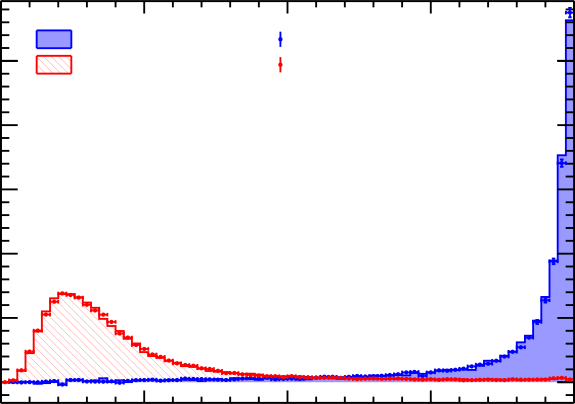
\includegraphics[width=0.9\textwidth]{BsDsK_TD/BDT/BDTG_Training_classifier_output}};
        \begin{scope}[x={(image.south east)},y={(image.north west)}]
            \foreach \x in {0, ..., 4}
                \tikzmath{\xtext = \x / 2 - 1; \xcoord = \x / 4;}
                \node at (\xcoord, -0.035) {\(\pgfmathprintnumber[fixed,precision=1,fixed zerofill=true]{\xtext}\)};
            \foreach \y in {0, ..., 5}
                \tikzmath{\ytext = \y / 20; \ycoord = \y / 6.28 + 0.055;}
                \node[anchor=east] at (0.005, \ycoord) {\(\pgfmathprintnumber[fixed,precision=2,fixed zerofill=true]{\ytext}\)};
            \node[anchor=east] at (1.0, -0.10) {BDT~response};
            \node[rotate=90,anchor=east,inner xsep=0pt,outer xsep=0pt] at (-0.09, 1.0) {Fraction of events};
            \node[anchor=west] at (0.13, 0.9) {Signal BDT~1};
            \node[anchor=west] at (0.13, 0.835) {Background BDT~1};
            \node[anchor=west] at (0.50, 0.9) {Signal BDT~2};
            \node[anchor=west] at (0.50, 0.835) {Background BDT~2};
        \end{scope}
    \end{tikzpicture}
    \caption{
        Output of the~BDTs when each is applied to the sample on which the other was trained.
        The two signal BDT~distributions (blue) match, as well as the two background distributions~(red), showing that neither~BDT was overtrained on specific features of its respective sample.}
    \label{fig:BsDsK_TD_BDTResponse}
\end{figure}

\subsection{\BsDsK~and \BsDsPi~signal candidates selection} \label{sec:BsDsK_TD_Selection_Signal}
Further selection of signal events is based on kinematic properties and identification of the candidates.
Selection criteria vary per \Dsm~decay mode, as summarised in \cref{tab:BsDsK_TD_Ds_Selection}.
For the \DsmKKPi~mode, the sample is split into three submodes, representing the decays \DsmPhiPi~(\PhiKK), \DsmKstK~(\KstKPi), and nonresonant \DsmKKPi~decays.
These have different PID~requirements: the resonances are relatively clean of background, justifying looser requirements on their daughter particles.
In contrast, the selection requirements on the nonresonant sample are stricter.
Each candidate only belongs to one of these categories; \ie if one is categorised as \DsmPhiPi~it is never classified as \DsmKstK, and if one is categorised as \DsmKstK it is not considered nonresonant, even if it would also satisfy the criteria for that submode.

Misidentified \DmKPiPi~(\LcmPKPi)~candidates are suppressed by vetoing any \Dsm~(\Lcm)~candidates whose mass in the \KpPimPim~(\PbarKPi)~mass hypothesis is close to the \Dm~(\Lcm)~mass, unless the~PID by itself is good enough (as specified in \cref{tab:BsDsK_TD_Ds_Selection}) to suppress misidentification.
Mode-independent selection criteria, as well as criteria on the \Bs~candidate (combination of \Dsm~candidate with a companion track), are listed in \cref{tab:BsDsK_TD_Selection}.
%
\begin{table}[htbp] \centerfloat
    \caption{
        Mode-dependent kinematic and PID~selection requirements for the \Dsm~candidates.
        The same selection is applied to the charge-conjugated candidates.}
    \label{tab:BsDsK_TD_Ds_Selection}
    \begin{tabular}{lll}
        \toprule
        Description & Variable & Requirement\tabularnewline
        \midrule
        \multicolumn{3}{l}{\DsmKKPi} \tabularnewline
        \midrule

        \Dsm~vertex separation & \chisq~w.r.t. \Bs~vertex & \(> \num{2}\) \tabularnewline
        \rowcolor{tableshade}\Dz~veto & \(m(\Km\Kp)\) & \(< \SI{1840}{\MeVcc}\) \tabularnewline

        \Dm~veto & mass under \({\pim\Kp\pim}\)~hypothesis & \(\notin \SI[parse-numbers=false]{[1840, 1900]}{\MeVcc}\) \tabularnewline
        \aligncell{r}{\emph{or}} & \(\dllkpi(\Km)\) & \(> \num{10}\) \tabularnewline

        \rowcolor{tableshade}\Lcm~veto & mass under \PbarKPi~hypothesis & \(\notin \SI[parse-numbers=false]{[2255, 2315]}{\MeVcc}\) \tabularnewline
        \rowcolor{tableshade}\aligncell{r}{\emph{or}} & \(\dllkp(\Km)\) & \(< \num{5}\) \tabularnewline
        \multicolumn{3}{l}{Submodes} \tabularnewline

        \quad\DsmPhiPi & \(m(\Km\Kp)\) & \(\in \SI[parse-numbers=false]{[1000, 1040]}{\MeVcc}\) \tabularnewline
        \aligncell{r}{\emph{and}} & \(\dllkpi(\Kmp)\) & \(> \num{-2}\) \tabularnewline

        \rowcolor{tableshade}\quad\DsmKstK & \(m(\Kp\pim)\) & \(\in \SI[parse-numbers=false]{[842, 942]}{\MeVcc}\) \tabularnewline
        \rowcolor{tableshade}\aligncell{r}{\emph{and}} & \(\dllkpi(\Kp)\) & \(> \num{-2}\) \tabularnewline
        \rowcolor{tableshade}\aligncell{r}{\emph{and}} & \(\dllkpi(\Km)\) & \(> \num{5}\) \tabularnewline

        \quad Nonresonant & \(\dllkpi(\Kmp)\) & \(> \num{5}\) \tabularnewline
        \aligncell{r}{\emph{and}} & \(\dllkpi(\pim)\) & \(< \num{10}\) \tabularnewline[1ex]

        \midrule
        \multicolumn{3}{l}{\DsmKPiPi} \tabularnewline
        \midrule

        \Dsm~vertex separation & \chisq~w.r.t. \Bs~vertex & \(> \num{9}\) \tabularnewline
        \rowcolor{tableshade}\Dz~veto & \(m(\Km\pip)\) & \(< \SI{1750}{\MeVcc}\) \tabularnewline

        \Dm~veto & mass under \({\pim\Kp\pim}\)~hypothesis & \(\notin \SI[parse-numbers=false]{[1840, 1900]}{\MeVcc}\) \tabularnewline
        \aligncell{r}{\emph{or}} & \(\dllkpi(\Km)\) & \(> \num{20}\) \tabularnewline
        \aligncell{r}{\emph{or}} & \(\dllkpi(\pip)\) & \(< \num{-10}\) \tabularnewline

        \rowcolor{tableshade}\Lc~veto & mass under \PbarKPi~hypothesis & \(\notin \SI[parse-numbers=false]{[2255, 2315]}{\MeVcc}\) \tabularnewline
        \rowcolor{tableshade}\aligncell{r}{\emph{or}} & \(\dllkp(\Km)\) & \(< \num{5}\) \tabularnewline

        PID~requirements & \(\dllkpi(\Km)\) & \(> \num{10}\) \tabularnewline
        \aligncell{r}{\emph{and}} & \(\dllkpi(\pipm)\) & \(< \num{5}\) \tabularnewline
        \aligncell{r}{\emph{and}} & \(\dllkp(\pipm)\) & \(< \num{10}\) \tabularnewline[1ex]

        \midrule
        \multicolumn{3}{l}{\DsmPiPiPi} \tabularnewline
        \midrule
        \Dsm~vertex separation & \chisq~w.r.t. \Bs~vertex & \(> \num{9}\) \tabularnewline
        \rowcolor{tableshade}\Dz~veto & \(m(\pim\pip)\)~(both combinations) & \(< \SI{1700}{\MeVcc}\) \tabularnewline

        PID~requirements & \(\dllkpi(\pimp)\)~(for each pion) & \(< \num{10}\) \tabularnewline
        \aligncell{r}{\emph{and}} & \(\dllkp(\pimp)\)~(for each pion) & \(< \num{10}\) \tabularnewline
        \bottomrule
    \end{tabular}
\end{table}
%
\begin{table}[htb] \centerfloat
    \caption{
        Mode-independent kinematic and PID~selection requirements for the \BsDsK~and \BsDsPi~candidates.
        The \Dsmp~candidates are reconstructed as specified in \cref{tab:BsDsK_TD_Ds_Selection}, and the companion track is the \Kpm~or \pipm~candidate that is combined with the \Dsmp~candidate form the \Bs~candidate.}
    \label{tab:BsDsK_TD_Selection}
    \begin{tabular}{lll}
        \toprule
        Description & Variable & Requirement\tabularnewline
        \midrule
        \Bs~decay time & decay time w.r.t.~PV & \(> \SI{0.4}{\ps}\) \tabularnewline
        \rowcolor{tableshade}\Bs~invariant mass & \({m(\Bs)}\) & \(\in \SI[parse-numbers=false]{[5300, 5800]}{\MeVcc}\) \tabularnewline
        Companion~PID & \({\dllkpi(\text{companion})}\) & \(< \num{0}\) for the \pion~hypothesis \tabularnewline
        & & \(> \num{5}\) for the \kaon~hypothesis \tabularnewline
        \rowcolor{tableshade}Semileptonic veto & \(\dllmupi(\text{companion})\) & \(< \num{2}\) \tabularnewline
        \midrule
        \Dsmp~decay time & decay time w.r.t. \Bs~vertex & \(> \num{0}\) \tabularnewline
        \rowcolor{tableshade}\Dsmp~invariant mass & \({m(\Dsmp)}\) & \(\in \SI[parse-numbers=false]{[1930, 2015]}{\MeVcc}\) \tabularnewline
        \bottomrule
    \end{tabular}
\end{table}

\subsection{\BdDPi~control channel selection}

The selection of \BdDPi~candidates proceeds analogous to that of \BsDsK~and \BsDsPi~candidates, except there is only one mode,~\DmKPiPi.
The requirements on the candidates for this final state consist of several kinematic selection requirements and vetoes, which are listed in \cref{tab:BsDsK_TD_D_Selection}.
There are no PID requirements imposed on this sample, as this would only slightly increase the purity of this already very pure sample, while introducing biases in the data-simulation differences investigated using this decay.
%
\begin{table}[htb] \centerfloat
    \caption{
        Kinematic selection requirements for the~\BdDPi, \DmKPiPi~candidates.
        The same selection is applied to the charge-conjugated candidates.
        Requirements marked with~\(^\ast\)~apply separately for each~\pim.}
    \label{tab:BsDsK_TD_D_Selection}
    \hspace*{-.75cm}
    \begin{tabular}{lll}
        \toprule
        Description & Variable & Requirement\tabularnewline
        \midrule
        \DmPip~invariant mass & \({m(\DmPip)}\) & \(\in \SI[parse-numbers=false]{[5000, 6000]}{\MeVcc}\) \tabularnewline
        \rowcolor{tableshade}Semileptonic veto & \dllmupi(companion) & \(> \num{2}\) \tabularnewline
        \midrule
        \Dm~decay time & decay time w.r.t. \Bd~vertex & \(> \num{0}\) \tabularnewline
        \rowcolor{tableshade}\Dm~invariant mass & \(m(\KpPimPim)\) & \(\in \SI[parse-numbers=false]{[1830, 1920]}{\MeVcc}\) \tabularnewline
        \Dm~vertex separation & \chisq~w.r.t. \Bd~vertex & \(> \num{9}\) \tabularnewline

        \rowcolor{tableshade}\Dsm~veto\(^\ast\) & mass under \({\Km\Kp\pim}\)~hypothesis & \(\notin \SI[parse-numbers=false]{[1950, 2030]}{\MeVcc}\) \tabularnewline
        \rowcolor{tableshade}\aligncell{r}{\emph{or}} & \(\dllkpi(\pim)\) & \(< \num{0}\) \tabularnewline

        \Lcm~veto\(^\ast\) & mass under \PbarKPi~hypothesis & \(\notin \SI[parse-numbers=false]{[2255, 2315]}{\MeVcc}\) \tabularnewline
        \aligncell{r}{\emph{or}} & \(\dllkp(\pim)\) & \(< \num{0}\) \tabularnewline
        \bottomrule
    \end{tabular}
\end{table}

\clearpage
\section{Simulation} \label{sec:TD_DsK_Simulation}

\subsection{Simulated samples}
Several simulated samples are used in the analysis for selection, normalisation and background studies.
A full list of these simulated samples is given in \cref{tab:BsDsK_TD_MC_Samples}.
All of them are produced as described in \cref{sec:simulation} and subsequently processed with the same selection criteria applied as the real data.
%
\begin{table}[htbp] \centerfloat
    \caption{
        Simulated samples used for selection, normalisation, and the extraction of signal and background models for the different observables.
        Samples marked with~\(^\ast\)~are generated with \CP~violation, to verify that the correct \CP-violation parameters are determined in the analysis (the \emph{closure test} described in \cref{sec:BsDsK_TD_Syst}).
        Samples marked with~\(^\dagger\)~are also used for the flavour tagging calibration (see \cref{sec:BsDsK_TD_Tagging}), and the one marked with~\(^\ddagger\)~is also used for data-simulation corrections (\cref{sec:TD_DsK_Simulation_Corrections}).
        The ones marked with~\(^\S\)~are used for determining corrections on the decay-time acceptance description (see \cref{sec:BsDsK_TD_Acceptance}).
        Note that the \BsDsK~samples are used for background modelling under the \BsDsPi~signal (and vice versa).}
    \label{tab:BsDsK_TD_MC_Samples}
    \rowcolors{2}{tableshade}{}
    \sisetup{table-number-alignment=right}
    \begin{tabular}{llS[table-format=1.2e1]c}
        \toprule
        Sample    & Daughter decay & {Sample size} & Usage \tabularnewline
        \midrule
        \BsDsPi   & \DsmKKPi       & 1.25e6        & {\footnotesize{Background modelling\(^{\dagger\S}\)}} \tabularnewline
        \BsDsPi   & \DsmKPiPi      & 2.39e5        & {\footnotesize{Background modelling\(^{\dagger\S}\)}} \tabularnewline
        \BsDsPi   & \DsmPiPiPi     & 2.44e5        & {\footnotesize{Background modelling\(^{\dagger\S}\)}} \tabularnewline

        \BsDsK    & \DsmpKKPi      & 1.13e6        & {\footnotesize{Background modelling\(^\S\)}} \tabularnewline
        \BsDsK    & \DsmpKPiPi     & 2.18e5        & {\footnotesize{Background modelling\(^\S\)}} \tabularnewline
        \BsDsK    & \DsmpPiPiPi    & 3.10e5        & {\footnotesize{Background modelling\(^\S\)}} \tabularnewline

        \BsDsK    & \DsmpKKPi      & 5.12e6        & {\footnotesize{Closure test\(^\ast\)}} \tabularnewline
        \BsDsK    & \DsmpKPiPi     & 5.63e5        & {\footnotesize{Closure test\(^\ast\)}} \tabularnewline
        \BsDsK    & \DsmpPiPiPi    & 1.02e6        & {\footnotesize{Closure test\(^\ast\)}} \tabularnewline

        \BsDsstPi & \DsmKKPi       & 2.10e6        & {\footnotesize{Background modelling}} \tabularnewline
        \BsDsRho  & \DsmKKPi       & 2.07e6        & {\footnotesize{Background modelling}} \tabularnewline

        \LbDsP    & \DsmKKPi       & 5.07e5        & {\footnotesize{Background modelling}} \tabularnewline
        \LbDsstP  & \DsmKKPi       & 5.73e5        & {\footnotesize{Background modelling}} \tabularnewline
        \LbLcPi   & \LcPKPi        & 4.90e5        & {\footnotesize{Background modelling}} \tabularnewline
        \LbLcK    & \LcPKPi        & 5.43e5        & {\footnotesize{Background modelling}} \tabularnewline

        \BdDPi    & \DmKPiPi       & 3.34e6        & {\footnotesize{Background modelling\(^\ddagger\)}}\tabularnewline
        \BdDK     & \DmKPiPi       & 2.77e5        & {\footnotesize{Background modelling}} \tabularnewline
        \bottomrule
    \end{tabular}
\end{table}

\subsection{Simulation corrections} \label{sec:TD_DsK_Simulation_Corrections}

The abundant channel \BdDPi~is used to calibrate differences between data and simulation.
To do this, first of all, a pure \BdDPi~data sample is required.
This is obtained by conducting an extended maximum likelihood fit on the \DmpPipm~invariant mass spectrum, after which the background is statistically subtracted using the \sfit~method~\cite{Yuehong_sFit}.
The resulting \BdDPi~sample is then compared to the simulated signal sample of the same channel.
As an additional result, the yield of this channel is determined in this fit, and can be used in the fits with a \Dsm~meson in the final state to predict the amount of misidentified \BdDPi~decays remaining in those fits.

The fit on \BdDPi~is performed in the range \({m(\DmpPipm) \in \SI[parse-numbers=false]{[5000, 6000]}{\MeVcc}}\), and is performed separately for each combination of centre-of-mass energy~(\({\sqs = \SI[parse-numbers=false]{7,\ 8}{\TeV}}\)) and \lhcb~magnet polarity (four fits total).
The signal is parameterised using a double Crystal~Ball~(DCB) function (see \cref{sec:MassFits_Signal}).
All parameters for that shape, except the common mean and widths, are determined from a DCB~fit to the simulated \BdDPi~sample, and fixed in the fit to data.
The values of these parameters are listed in \cref{tab:BsDsK_TD_BdDPi_MC_Fit_Results}.
The mean~\DCBmu is left free in the data fit.
For the widths~\DCBsLR, a shared, floating mass~resolution scale~factor~\(R\) is applied to the values obtained from simulation.

The physical backgrounds (see \cref{sec:MassFits}) considered in the fit are the misidentified decays~\BdDK, \BsDsPi, and~\LbLcPi, and the partially reconstructed decays~\BdDRho and~\BdDstPi.
For each of those backgrounds, the shape is obtained from the respective simulated sample by applying the same selection to it and describing the shape using kernel estimation (see \cref{sec:methods_KernelEstimation}).
This method uses kernel~estimation to numerically generate a smooth~PDF from an arbitrary distribution.
The yield of each background decay is left floating in the fit, with the exception of the low-yield channels~\BsDsPi and~\LbLcPi, which are fixed to their predicted yields, in order to improve the fit quality.
Finally, the combinatorial background is modelled using a double negative exponential, representing the contributions of real \Dsmp~candidates combined with a random track and random four-track combinations.

This amounts to ten free parameters in total: the \BdDPi~signal yield, three background yields, the combinatorial yield, the signal mean mass, the two slopes of the combinatorial shapes and the relative fraction between their yields, and the mass resolution scale factor~\(R\).
The results of the fit are listed in \cref{tab:BsDsK_TD_BdDPi_Data_Fit_Results} and shown in \cref{fig:BsDsK_TD_BdDPi_Fit}.
%
\begin{table}[htb] \centerfloat
    \caption{
        Parameters of the DCB~function parameterising the \BdDPi~signal mass shape as obtained from a fit a simulated sample.
        The Crystal~Ball parameters are defined as described in \cref{sec:MassFits}.}
    \label{tab:BsDsK_TD_BdDPi_MC_Fit_Results}
    \rowcolors{2}{tableshade}{}
    \begin{tabular}{lS[table-format=4.3(3), table-number-alignment=right]}
        \toprule
        Parameter                      & \aligncell{r}{Fitted value} \tabularnewline
        \midrule
        \(\DCBmu_{\Bd}\)~(\si{\MeVcc}) & 5280.10  +- 0.05  \tabularnewline
        \(\DCBsL\)~(\si{\MeVcc})       &   21.587 +- 0.81  \tabularnewline
        \(\DCBsR\)~(\si{\MeVcc})       &   12.81  +- 0.19  \tabularnewline
        \DCBaL                         &   -2.136 +- 0.052 \tabularnewline
        \DCBaR                         &    2.005 +- 0.052 \tabularnewline
        \DCBnL                         &    2.592 +- 0.171 \tabularnewline
        \DCBnR                         &    1.107 +- 0.042 \tabularnewline
        \DCBf                          &    0.694 +- 0.032 \tabularnewline
        \bottomrule
    \end{tabular}
\end{table}

\begin{landscape}
\begin{table}[htbp] \centerfloat
    \caption{
        Fitted parameters from the mass fit to the \BdDPi~data sample.
        The \(N\)~parameters are the yields of the signal and background components and \(\DCBmu_{\Bd}\)~is the mean of the double Crystal Ball used to describe the \Bd~mass.
        The slopes~\(s_{\text{comb}}\) parameterise the exponential shapes describing the combinatorial background, and are given in units of~\num{e-3}, and \(f_{\text{comb}}\)~represents the fraction between them.
        The parameter~\(R\) is the ratio of the signal widths between data and simulation.
        The fit is split according to centre-of-mass energy and \lhcb~magnet polarity.}
    \label{tab:BsDsK_TD_BdDPi_Data_Fit_Results}
    \rowcolors{1}{}{tableshade}
    \sisetup{table-number-alignment=right}
    \begin{tabular}{l*{2}{S[table-format=5.3(3)]}*{2}{S[table-format=6.3(3)]}}
        \hiderowcolors \toprule
        \multirow{2}{*}[-2pt]{Fit parameters} & \multicolumn{2}{c}{\({\sqs = \SI{7}{\TeV}}\)} & \multicolumn{2}{c}{\({\sqs = \SI{8}{\TeV}}\)} \tabularnewline
        \cmidrule(lr){2-3}\cmidrule(lr){4-5}
                                              & {magnet up}       & {magnet down}     & {magnet up}        & {magnet down} \tabularnewline
        \showrowcolors \midrule
        \(N_{\BdDPi}\)                        & 66534   +- 282    & 95058 +- 336      & 200128    +- 487   & 203110    +-  491 \tabularnewline[.4ex]
        \(N_{\BdDRho}\)                       & 31975   +- 595    & 45276 +- 701      &  89806    +- 1027  &  95252    +- 1027 \tabularnewline[.4ex]
        \(N_{\BdDstPi}\)                      & 14149   +- 522    & 20189 +- 617      &  45845    +- 906   &  43553    +-  906 \tabularnewline[.4ex]
        \(N_{\BdDK}\)                         &  6339   +- 167    &  8186 +- 196      &  17953    +- 289   &  17652    +-  289 \tabularnewline[.4ex]
        \(N_{\text{comb}}\)                   & 18251   +- 307    & 25946 +- 362      &  61477    +- 541   &  60644    +-  533 \tabularnewline[.4ex]
        \(\DCBmu_{\Bd}\)~(\si{\MeVcc})        &  5278.20 +- 0.08  &  5278.24 +- 0.07  &   5278.21 +- 0.05  &   5278.10 +- 0.05 \tabularnewline[.4ex]
        \(s_{\text{comb}} \times \num{e3}\)   &    -0.44 +- 0.35  &     0.00 +- 0.03  &      0.00 +- 0.00  &     -0.04 +- 0.06  \tabularnewline[.4ex]
        \(s_{\text{comb}} \times \num{e3}\)   &    -6.56 +- 0.31  &    -6.14 +- 0.17  &     -6.11 +- 0.11  &     -6.04 +- 0.11  \tabularnewline[.4ex]
        \(f_{\text{comb}}\)                   &     0.176+- 0.030 &     0.140+- 0.013 &      0.154+- 0.008 &      0.157+- 0.005 \tabularnewline[.4ex]
        \(R\)                                 &     1.130+- 0.005 &     1.131+- 0.004 &      1.121+- 0.003 &      1.124+- 0.003 \tabularnewline[.4ex]
        \hiderowcolors \midrule
        \multirow{2}{*}{Fixed Parameters} \tabularnewline\tabularnewline
        \midrule
        \(N_{\BsDsPi}\)                       & \centercell{1000}    & \centercell{1000}    & \centercell{2000}    & \centercell{2000} \tabularnewline[.4ex]
        \rowcolor{tableshade}
        \(N_{\LbLcPi}\)                       & \centercell{ 250}    & \centercell{ 250}    & \centercell{ 500}    & \centercell{ 500} \tabularnewline[.4ex]
        \bottomrule
    \end{tabular}
\end{table}
\end{landscape}
%
\begin{figure}[htb] \centerfloat
    \fontsize{7}{8.4}\selectfont
    \begin{subfigure}{.48\textwidth} \centerfloat
        \begin{tikzpicture}
            \node[anchor=south west,inner sep=0] (image) at (0,0) {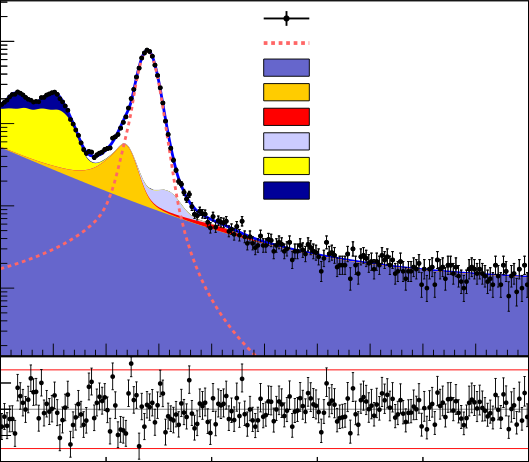
\includegraphics[width=0.9\textwidth]{BsDsK_TD/BdDPi_Fit/mass_Bd2DPi_BeautyMass_up_kpipi_2011}};
            \begin{scope}[x={(image.south east)},y={(image.north west)}]
                \foreach \x/\xtext in {5000, 5200, ..., 6000}
                {
                    \tikzmath{\xpos = (\x - 5000) / 1000;}
                    \node at (\xpos, -0.025) {\(\xtext\)};
                }
                \node[anchor=base east] at (0.005, 0.363) {\(10\)};
                \node[anchor=base east] at (0.005, 0.363+1*.178) {\(10^{2}\)};
                \node[anchor=base east] at (0.005, 0.363+2*.178) {\(10^{3}\)};
                \node[anchor=base east] at (0.005, 0.363+3*.178) {\(10^{4}\)};
                \foreach \p/\ptext in {-2, 0, 2}
                {
                    \tikzmath{\ypos = ((2 + \p) / 2 + 1) * (0.228 / 4);}
                    \node[anchor=east] at (0.005, \ypos) {\(\scriptstyle\ptext\)};
                }
                \node[anchor=east] at (1.0, -0.09) {\({m(\DmpPipm)}~[\si{\MeVcc}]\)};
                \node[rotate=90,anchor=east,inner xsep=0pt,outer xsep=0pt] at (-0.13, 1.0) {\({\text{Candidates}/(\SI{10}{\MeVcc})}\)};
                \node[anchor=east] at (0.26, 0.92) {\large\lhcb};
                % Legend
                {
                    \fontsize{5.5}{6.6}\selectfont
                    \node[anchor=base west] at (0.58, 0.946) {Data};
                    \node[anchor=base west] at (0.58, 0.946 - 1 * 0.0532) {\BdDPi~signal};
                    \node[anchor=base west] at (0.58, 0.946 - 2 * 0.0532) {Combinatorial};
                    \node[anchor=base west] at (0.58, 0.946 - 3 * 0.0532) {\BdDK};
                    \node[anchor=base west] at (0.58, 0.946 - 4 * 0.0532) {\LbLcPi};
                    \node[anchor=base west] at (0.58, 0.946 - 5 * 0.0532) {\BsDsPi};
                    \node[anchor=base west] at (0.58, 0.946 - 6 * 0.0532) {\BdDRho};
                    \node[anchor=base west] at (0.58, 0.946 - 7 * 0.0532) {\BdDstPi};
                }
            \end{scope}
        \end{tikzpicture}
        \caption{\({\sqs = \SI{7}{\TeV}}\), \lhcb~magnet up.}
    \end{subfigure} \hfill%
    \begin{subfigure}{.48\textwidth} \centerfloat
        \begin{tikzpicture}
            \node[anchor=south west,inner sep=0] (image) at (0,0) {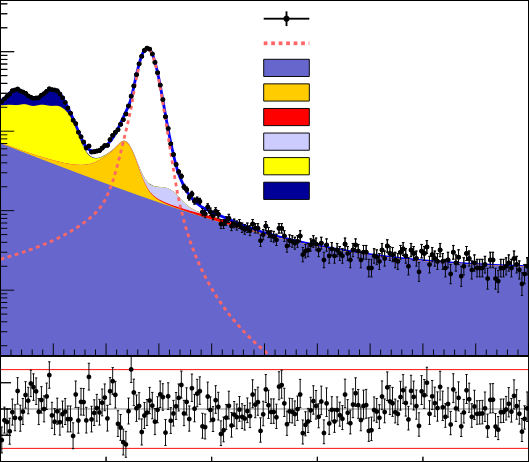
\includegraphics[width=0.9\textwidth]{BsDsK_TD/BdDPi_Fit/mass_Bd2DPi_BeautyMass_down_kpipi_2011}};
            \begin{scope}[x={(image.south east)},y={(image.north west)}]
                \foreach \x/\xtext in {5000, 5200, ..., 6000}
                {
                    \tikzmath{\xpos = (\x - 5000) / 1000;}
                    \node at (\xpos, -0.025) {\(\xtext\)};
                }
                \node[anchor=base east] at (0.005, 0.358) {\(10\)};
                \node[anchor=base east] at (0.005, 0.358+1*.171) {\(10^{2}\)};
                \node[anchor=base east] at (0.005, 0.358+2*.171) {\(10^{3}\)};
                \node[anchor=base east] at (0.005, 0.358+3*.171) {\(10^{4}\)};
                \foreach \p/\ptext in {-2, 0, 2}
                {
                    \tikzmath{\ypos = ((2 + \p) / 2 + 1) * (0.228 / 4);}
                    \node[anchor=east] at (0.005, \ypos) {\(\scriptstyle\ptext\)};
                }
                \node[anchor=east] at (1.0, -0.09) {\({m(\DmpPipm)}~[\si{\MeVcc}]\)};
                \node[rotate=90,anchor=east,inner xsep=0pt,outer xsep=0pt] at (-0.13, 1.0) {\({\text{Candidates}/(\SI{10}{\MeVcc})}\)};
                \node[anchor=east] at (0.26, 0.92) {\large\lhcb};
                % Legend
                {
                    \fontsize{5.5}{6.6}\selectfont
                    \node[anchor=base west] at (0.58, 0.946) {Data};
                    \node[anchor=base west] at (0.58, 0.946 - 1 * 0.0532) {\BdDPi~signal};
                    \node[anchor=base west] at (0.58, 0.946 - 2 * 0.0532) {Combinatorial};
                    \node[anchor=base west] at (0.58, 0.946 - 3 * 0.0532) {\BdDK};
                    \node[anchor=base west] at (0.58, 0.946 - 4 * 0.0532) {\LbLcPi};
                    \node[anchor=base west] at (0.58, 0.946 - 5 * 0.0532) {\BsDsPi};
                    \node[anchor=base west] at (0.58, 0.946 - 6 * 0.0532) {\BdDRho};
                    \node[anchor=base west] at (0.58, 0.946 - 7 * 0.0532) {\BdDstPi};
                }
            \end{scope}
        \end{tikzpicture}
        \caption{\({\sqs = \SI{7}{\TeV}}\), \lhcb~magnet down.}
    \end{subfigure}
    \\[4ex]
    \begin{subfigure}{.48\textwidth} \centerfloat
        \begin{tikzpicture}
            \node[anchor=south west,inner sep=0] (image) at (0,0) {\includegraphics[width=0.9\textwidth]{BsDsK_TD/BdDPi_Fit/mass_Bd2DPi_BeautyMass_up_kpipi_2012}};
            \begin{scope}[x={(image.south east)},y={(image.north west)}]
                \foreach \x/\xtext in {5000, 5200, ..., 6000}
                {
                    \tikzmath{\xpos = (\x - 5000) / 1000;}
                    \node at (\xpos, -0.025) {\(\xtext\)};
                }
                \node[anchor=base east] at (0.005, 0.348) {\(10\)};
                \node[anchor=base east] at (0.005, 0.348 + 1 * .160) {\(10^{2}\)};
                \node[anchor=base east] at (0.005, 0.348 + 2 * .160) {\(10^{3}\)};
                \node[anchor=base east] at (0.005, 0.348 + 3 * .160) {\(10^{4}\)};
                \foreach \p/\ptext in {-2, 0, 2}
                {
                    \tikzmath{\ypos = ((2 + \p) / 2 + 1) * (0.228 / 4);}
                    \node[anchor=east] at (0.005, \ypos) {\(\scriptstyle\ptext\)};
                }
                \node[anchor=east] at (1.0, -0.09) {\({m(\DmpPipm)}~[\si{\MeVcc}]\)};
                \node[rotate=90,anchor=east,inner xsep=0pt,outer xsep=0pt] at (-0.13, 1.0) {\({\text{Candidates}/(\SI{10}{\MeVcc})}\)};
                \node[anchor=east] at (0.26, 0.92) {\large\lhcb};
                % Legend
                {
                    \fontsize{5.5}{6.6}\selectfont
                    \node[anchor=base west] at (0.58, 0.946) {Data};
                    \node[anchor=base west] at (0.58, 0.946 - 1 * 0.0532) {\BdDPi~signal};
                    \node[anchor=base west] at (0.58, 0.946 - 2 * 0.0532) {Combinatorial};
                    \node[anchor=base west] at (0.58, 0.946 - 3 * 0.0532) {\BdDK};
                    \node[anchor=base west] at (0.58, 0.946 - 4 * 0.0532) {\LbLcPi};
                    \node[anchor=base west] at (0.58, 0.946 - 5 * 0.0532) {\BsDsPi};
                    \node[anchor=base west] at (0.58, 0.946 - 6 * 0.0532) {\BdDRho};
                    \node[anchor=base west] at (0.58, 0.946 - 7 * 0.0532) {\BdDstPi};
                }
            \end{scope}
        \end{tikzpicture}
        \caption{\({\sqs = \SI{8}{\TeV}}\), \lhcb~magnet up.}
    \end{subfigure} \hfill%
    \begin{subfigure}{.48\textwidth} \centerfloat
        \begin{tikzpicture}
            \node[anchor=south west,inner sep=0] (image) at (0,0) {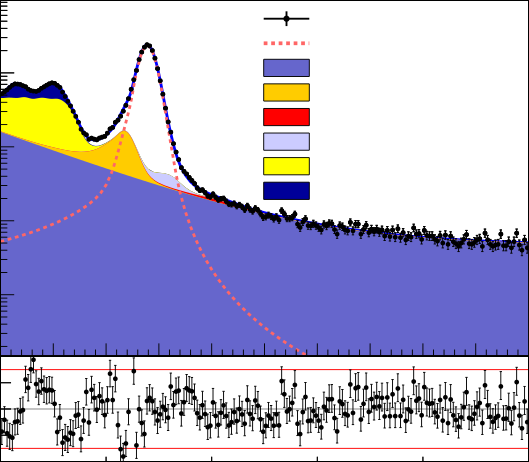
\includegraphics[width=0.9\textwidth]{BsDsK_TD/BdDPi_Fit/mass_Bd2DPi_BeautyMass_down_kpipi_2012}};
            \begin{scope}[x={(image.south east)},y={(image.north west)}]
                \foreach \x/\xtext in {5000, 5200, ..., 6000}
                {
                    \tikzmath{\xpos = (\x - 5000) / 1000;}
                    \node at (\xpos, -0.025) {\(\xtext\)};
                }
                \node[anchor=base east] at (0.005, 0.348) {\(10\)};
                \node[anchor=base east] at (0.005, 0.348 + 1 * .160) {\(10^{2}\)};
                \node[anchor=base east] at (0.005, 0.348 + 2 * .160) {\(10^{3}\)};
                \node[anchor=base east] at (0.005, 0.348 + 3 * .160) {\(10^{4}\)};
                \foreach \p/\ptext in {-2, 0, 2}
                {
                    \tikzmath{\ypos = ((2 + \p) / 2 + 1) * (0.228 / 4);}
                    \node[anchor=east] at (0.005, \ypos) {\(\scriptstyle\ptext\)};
                }
                \node[anchor=east] at (1.0, -0.09) {\({m(\DmpPipm)}~[\si{\MeVcc}]\)};
                \node[rotate=90,anchor=east,inner xsep=0pt,outer xsep=0pt] at (-0.13, 1.0) {\({\text{Candidates}/(\SI{10}{\MeVcc})}\)};
                \node[anchor=east] at (0.26, 0.92) {\large\lhcb};
                % Legend
                {
                    \fontsize{5.5}{6.6}\selectfont
                    \node[anchor=base west] at (0.58, 0.946) {Data};
                    \node[anchor=base west] at (0.58, 0.946 - 1 * 0.0532) {\BdDPi~signal};
                    \node[anchor=base west] at (0.58, 0.946 - 2 * 0.0532) {Combinatorial};
                    \node[anchor=base west] at (0.58, 0.946 - 3 * 0.0532) {\BdDK};
                    \node[anchor=base west] at (0.58, 0.946 - 4 * 0.0532) {\LbLcPi};
                    \node[anchor=base west] at (0.58, 0.946 - 5 * 0.0532) {\BsDsPi};
                    \node[anchor=base west] at (0.58, 0.946 - 6 * 0.0532) {\BdDRho};
                    \node[anchor=base west] at (0.58, 0.946 - 7 * 0.0532) {\BdDstPi};
                }
            \end{scope}
        \end{tikzpicture}
        \caption{\({\sqs = \SI{8}{\TeV}}\), \lhcb~magnet down.}
    \end{subfigure}
    \caption{
        Distributions of the \DmpPipm~invariant mass obtained in the fit to \BdDPi~candidates in data, split by centre-of-mass energy and \lhcb~magnet polarity.
        The solid, blue curve corresponds to the fit described in the text.
        Different contributions to the fit are shown as coloured areas (for backgrounds) or a dashed line (signal), as described in the legend in the figure.}
    \label{fig:BsDsK_TD_BdDPi_Fit}
\end{figure}

From the mass fit, a statistically pure signal sample is extracted using the \sfit~method~\cite{Yuehong_sFit}.
This sample is then compared to the simulated \BdDPi~sample.
This comparison is done in two variables that are relevant to the PID~performance: track momentum and total number of event tracks.

The resulting weights, obtained as the ratio between data and simulation, are shown in \cref{fig:BsDsK_TD_DataMC_Weights}.
In general, they correct for the particle multiplicities, which are too low in simulation.
These weights are applied to each simulated sample used throughout the rest of the analysis.
%
\begin{figure}[htb] \centerfloat
    \hspace*{-1.25cm}
    \fontsize{7}{8.4}\selectfont
    \begin{subfigure}{.45\textwidth} \centerfloat
        \begin{tikzpicture}
            \node[anchor=south west,inner sep=0] (image) at (0,0) {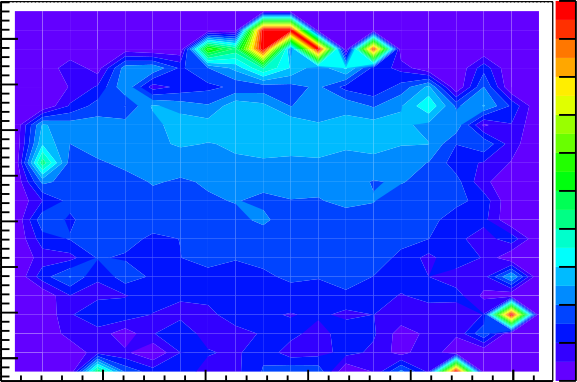
\includegraphics[width=0.9\textwidth]{BsDsK_TD/BdDPi_Fit/datamc_weights_p_nTracks_2011_up_filtered}};
            \begin{scope}[x={(image.south east)},y={(image.north west)}]
                \foreach \x/\xtext in {9, ..., 13}
                {
                    \tikzmath{\xpos = (\x - 9) / 5.62 + 0.18;}
                    \node at (\xpos, -0.045) {\(\xtext\)};
                }
                \foreach \y in {6, ..., 13}
                {
                    \tikzmath{\ypos = (\y - 5.6) / 8.5; \ytext = \y/2;}
                    \node[anchor=base east] at (0.0000, \ypos) {\(\ytext\)};
                }
                \foreach \z in {0, ..., 10}
                {
                    \tikzmath{\ztext = \z/2;}
                    \node[anchor=west] at (1.0, 0.01 + \z/10.15) {\(\pgfmathprintnumber[fixed,precision=1,fixed zerofill=true]{\ztext}\)};
                }
                \node[anchor=east] at (1.0, -0.14) {\(\log(\ptot/(\si{\GeVc}))\)};
                \node[rotate=90,anchor=east,inner xsep=0pt,outer xsep=0pt] at (-0.13, 1.0) {\(\log(\ntr)\)};
            \end{scope}
        \end{tikzpicture}
        \caption{\({\sqs = \SI{7}{\TeV}}\), \lhcb~magnet up.}
    \end{subfigure} \hfill%
    \begin{subfigure}{.45\textwidth} \centerfloat
        \begin{tikzpicture}
            \node[anchor=south west,inner sep=0] (image) at (0,0) {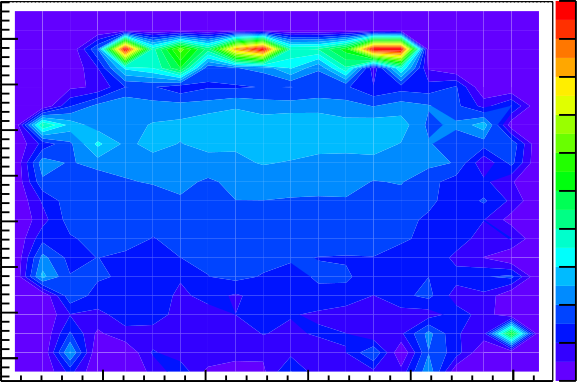
\includegraphics[width=0.9\textwidth]{BsDsK_TD/BdDPi_Fit/datamc_weights_p_nTracks_2011_dw_filtered}};
            \begin{scope}[x={(image.south east)},y={(image.north west)}]
                \foreach \x/\xtext in {9, ..., 13}
                {
                    \tikzmath{\xpos = (\x - 9) / 5.62 + 0.18;}
                    \node at (\xpos, -0.045) {\(\xtext\)};
                }
                \foreach \y in {6, ..., 13}
                {
                    \tikzmath{\ypos = (\y - 5.6) / 8.5; \ytext = \y/2;}
                    \node[anchor=base east] at (0.0000, \ypos) {\(\ytext\)};
                }
                \foreach \z in {0, ..., 10}
                {
                    \tikzmath{\ztext = \z/2;}
                    \node[anchor=west] at (1.0, 0.01 + \z/10.15) {\(\pgfmathprintnumber[fixed,precision=1,fixed zerofill=true]{\ztext}\)};
                }
                \node[anchor=east] at (1.0, -0.14) {\(\log(\ptot/(\si{\GeVc}))\)};
                \node[rotate=90,anchor=east,inner xsep=0pt,outer xsep=0pt] at (-0.13, 1.0) {\(\log(\ntr)\)};
            \end{scope}
        \end{tikzpicture}
        \caption{\({\sqs = \SI{7}{\TeV}}\), \lhcb~magnet down.}
    \end{subfigure}
    \\[4ex]
    \hspace*{-1.25cm}
    \begin{subfigure}{.45\textwidth} \centerfloat
        \begin{tikzpicture}
            \node[anchor=south west,inner sep=0] (image) at (0,0) {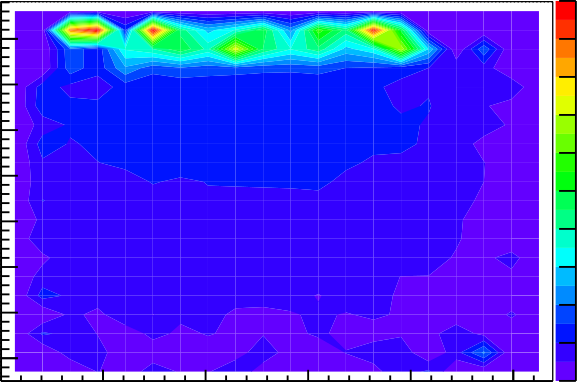
\includegraphics[width=0.9\textwidth]{BsDsK_TD/BdDPi_Fit/datamc_weights_p_nTracks_2012_up_filtered}};
            \begin{scope}[x={(image.south east)},y={(image.north west)}]
                \foreach \x/\xtext in {9, ..., 13}
                {
                    \tikzmath{\xpos = (\x - 9) / 5.62 + 0.18;}
                    \node at (\xpos, -0.045) {\(\xtext\)};
                }
                \foreach \y in {6, ..., 13}
                {
                    \tikzmath{\ypos = (\y - 5.6) / 8.5; \ytext = \y/2;}
                    \node[anchor=base east] at (0.0000, \ypos) {\(\ytext\)};
                }
                \foreach \z/\ztext in {0, ..., 10}
                    \node[anchor=west] at (1.0, 0.01 + \z/10.15) {\(\ztext\)};
                \node[anchor=east] at (1.0, -0.14) {\(\log(\ptot/(\si{\GeVc}))\)};
                \node[rotate=90,anchor=east,inner xsep=0pt,outer xsep=0pt] at (-0.13, 1.0) {\(\log(\ntr)\)};
            \end{scope}
        \end{tikzpicture}
        \caption{\({\sqs = \SI{8}{\TeV}}\), \lhcb~magnet up.}
    \end{subfigure} \hfill%
    \begin{subfigure}{.45\textwidth} \centerfloat
        \begin{tikzpicture}
            \node[anchor=south west,inner sep=0] (image) at (0,0) {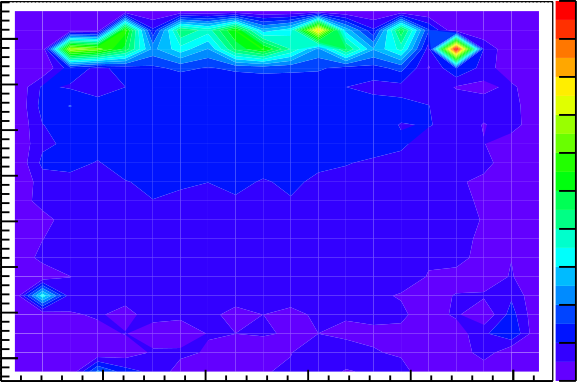
\includegraphics[width=0.9\textwidth]{BsDsK_TD/BdDPi_Fit/datamc_weights_p_nTracks_2012_dw_filtered}};
            \begin{scope}[x={(image.south east)},y={(image.north west)}]
                \foreach \x/\xtext in {9, ..., 13}
                {
                    \tikzmath{\xpos = (\x - 9) / 5.62 + 0.18;}
                    \node at (\xpos, -0.045) {\(\xtext\)};
                }
                \foreach \y in {6, ..., 13}
                {
                    \tikzmath{\ypos = (\y - 5.6) / 8.5; \ytext = \y/2;}
                    \node[anchor=base east] at (0.0000, \ypos) {\(\ytext\)};
                }
                \foreach \z/\ztext in {0, ..., 10}
                    \node[anchor=west] at (1.0, 0.01 + \z/10.15) {\(\ztext\)};
                \node[anchor=east] at (1.0, -0.14) {\(\log(\ptot/(\si{\GeVc}))\)};
                \node[rotate=90,anchor=east,inner xsep=0pt,outer xsep=0pt] at (-0.13, 1.0) {\(\log(\ntr)\)};
            \end{scope}
        \end{tikzpicture}
        \caption{\({\sqs = \SI{8}{\TeV}}\), \lhcb~magnet down.}
    \end{subfigure}
    \caption{
        Data/simulation ratios as obtained from the \BdDPi~fits as a function of track momentum~\ptot and number of tracks in the event~\ntr, split by centre-of-mass energy and \lhcb~magnet polarity.
        Differences between the ratios for different \lhcb~magnet polarities are possibly due to differences in the crossing angle of the proton beams.}
    \label{fig:BsDsK_TD_DataMC_Weights}
\end{figure}

\clearpage
\section{Signal extraction} \label{sec:BsDsK_TD_MD_Fit}

\subsection{Motivation} \label{sec:BsDsK_TD_MD_Fit_Motivation}

A pure sample of \BsDsK~events is required to extract the time-dependent \CP~observables.
This sample is obtained by fitting the data, including information on the various backgrounds present, and statistically subtracting the background.
In addition, a kinematically similar sample of \BsDsPi~events is extracted in the same way, and used for flavour tagging and decay-time acceptance calibration (see \cref{chp:BsDsK_TD}).

To identify signal events, three variables with good discriminating properties for the various event categories are selected: the \Bs~candidate mass, the \Dsmp~candidate mass, and the PID~information of the companion track~(\({\log|\dllkpi|}\)).
These three variables are simultaneously fitted using a multivariate, unbinned extended maximum likelihood fit.
Two separate fits are performed for the \BsDsPi~and \BsDsK~samples, which are split by~\dllkpi as specified in \cref{tab:BsDsK_TD_Selection}: \({< \num{0}}\)~for the pion companion, and \({> \num{5}}\)~for the kaon.
In the following sections, the definitions of signal, background and combinatorial shapes in each of the three variables are given.
Both fits are set up similarly, with some differences -- most notably in the treatment of backgrounds -- as discussed below.

\subsection{PID reweighting} \label{sec:BsDsK_TD_MD_PID_Reweighting}

The shapes of the mass distributions for the \Bs~and \Dsmp~candidates are readily extracted from simulated samples, but for the companion \dllkpi~distributions, the description in simulation is inadequate, and a more involved procedure is employed.
The starting point is the \dllkpi~shape for a control mode from data, namely \DstarDPi~for pure pion and kaon samples, and \Lzppi~for a pure proton sample~\cite{Powell:1322666}.
The background in each of these samples is subtracted using statistical weights, and the relevant \dllkpi~requirement (\({< \num{0}}\)~or \({> \num{5}}\))~is applied.
The sample is subsequently weighted to match the momentum and rapidity distributions of companion tracks from corresponding \Bs~decays.
These simulated samples are first weighted using the corrections obtained with the procedure from \cref{sec:TD_DsK_Simulation}, after which the data calibration sample is weighted to match the track momentum and the number of tracks in the event (or rather, the logarithm of those variables).
For \BsDsK, however, the shape of the track momentum does not yield well-behaved \dllkpi~shapes, and the track transverse momentum,~\({\log(\pt)}\), is used instead.
This weighting is performed separately for each centre-of-mass energy and magnet polarity, after which they are combined in ratios corresponding to the amount of luminosity in the data.
For each variable, twenty bins are used (\num{400}~bins total).
Several binning schemes have been examined, and the difference between the resulting distributions is found to be negligible.

Correlations between the \Bs~invariant mass, \Dsmp~invariant mass, and companion~\dllkpi have been studied to ensure that the extracted weights are correct.
Correlations between these variables and the decay time and per-event decay-time error, are also checked.
To investigate the effects of such correlations, large samples of background events have been generated using a phase-space generator.
Correlations between the fit variables and the decay-time variables are generally found to be of the order~\SI{5}{\percent}.
These correlations are slightly larger in some channels, up to about~\SI{25}{\percent} in a few of them.
All these correlations are accounted for in the systematic uncertainties by performing pseudo-experiments (see \cref{sec:BsDsK_TD_Syst}).

\subsection{Signal shape}

The signal shapes of the \Bs~and \Dsmp~invariant mass distributions are parameterised using a DCB~shape (see \cref{sec:MassFits_Signal}) with shared mean, with the fraction between the Gaussian distributions fixed to~\num{0.5}.
The tail parameters are obtained by fitting the corresponding simulated sample.
This is done separately for each of the five \Dsmp~final states, for both~\BsDsPi and~\BsDsK, and for both the \Bs~and \Dsmp~invariant masses (twenty fits total).
The results of those fits are shown in \cref{fig:BsDsK_TD_Signal_Shape_Results,tab:BsDsK_TD_Signal_Shape_Results}.
In the~PDF used in the multivariate fit, the mean is left floating to account for slight differences between data and simulation, and the mass resolution~\DCBs is scaled by a mass resolution scale factor~\(R\).
This parameter is shared among all \Dsmp~modes but separate for the \Bs~and \Dsmp~signal shapes, yielding two parameters \RBs~and \RDs~for each multivariate fit.

To obtain a shape for the \dllkpi~distribution of the companion candidates, the procedure described in \cref{sec:BsDsK_TD_MD_PID_Reweighting} is applied.
A calibration sample of the respective type of companion particle (pion or kaon) is taken, and reweighted to match the kinematics of the signal decay, as determined from simulation.
%
\begin{figure}[hp] \centerfloat
    \fontsize{7}{8.4}\selectfont
    \begin{subfigure}{.44\textwidth} \centerfloat
        \begin{tikzpicture}
            \node[anchor=south west,inner sep=0] (image) at (0,0) {\includegraphics[width=0.9\textwidth]{BsDsK_TD/Signal_Templates/BsDsK_BsMass}};
            \begin{scope}[x={(image.south east)},y={(image.north west)}]
                \foreach \x/\xtext in {5300, 5350, ..., 5500}
                {
                    \tikzmath{\xpos = (\x - 5300) / 200;}
                    \node at (\xpos, -0.025) {\(\xtext\)};
                }
                \node[anchor=base east] at (0.005, 0.107) {\num{e-4}};
                \node[anchor=base east] at (0.005, 0.107 + 1 * 0.301) {\num{e-3}};
                \node[anchor=base east] at (0.005, 0.107 + 2 * 0.301) {\num{e-2}};
                \node[anchor=east] at (1.0, -0.09) {\({m(\DsmpKpm)}~[\si{\MeVcc}]\)};
                \node[rotate=90,anchor=east,inner xsep=0pt,outer xsep=0pt] at (-0.13, 1.0) {PDF};
                \node[anchor=east] at (0.91, 0.92) {\large\lhcb};
            \end{scope}
        \end{tikzpicture}
        \caption{\Bs~mass.}
    \end{subfigure} \hfill%
    \begin{subfigure}{.44\textwidth} \centerfloat
        \begin{tikzpicture}
            \node[anchor=south west,inner sep=0] (image) at (0,0) {\includegraphics[width=0.9\textwidth]{BsDsK_TD/Signal_Templates/BsDsK_DsMass}};
            \begin{scope}[x={(image.south east)},y={(image.north west)}]
                \foreach \x/\xtext in {1940, 1960, ..., 2000}
                {
                    \tikzmath{\xpos = (\x - 1940) / (2000 - 1940) * (0.822 - 0.12) + 0.12;}
                    \node at (\xpos, -0.025) {\(\xtext\)};
                }
                \node[anchor=east] at (0.005, 0.) {\num{0}};
                \foreach \y in {1, ..., 6}
                {
                    \tikzmath{\ypos = \y / 6.13; \ytext = \y / 100;}
                    \node[anchor=east] at (0.005, \ypos) {\pgfmathprintnumber[fixed,precision=2,fixed zerofill=true]{\ytext}};
                }
                \node[anchor=east] at (1.0, -0.09) {\({m(\Dsmp)}~[\si{\MeVcc}]\)};
                \node[rotate=90,anchor=east,inner xsep=0pt,outer xsep=0pt] at (-0.14, 1.0) {PDF};
                \node[anchor=east] at (0.91, 0.92) {\large\lhcb};
            \end{scope}
        \end{tikzpicture}
        \caption{\Dsmp~mass.}
    \end{subfigure} \vspace{2ex}
    \begin{subfigure}{.70\textwidth} \centerfloat
        \begin{tikzpicture}[scale=0.9, every node/.style={scale=0.9}]
            \node[anchor=south west,inner sep=0] (image) at (0,0) {\includegraphics[width=0.9\textwidth]{BsDsK_TD/Signal_Templates/BsDsPi_CompDLLkpi}};
            \begin{scope}[x={(image.south east)},y={(image.north west)}]
                \node at (0.163, -0.025) {\num{-5}};
                \node at (0.583, -0.025) {\num{ 0}};
                \node at (1.  , -0.025) {\num{ 5}};
                \node[anchor=east] at (0.005, 0.) {\num{0}};
                \foreach \y in {1, ..., 5}
                {
                    \tikzmath{\ypos = \y / 5.07; \ytext = \y / 100;}
                    \node[anchor=east] at (0.005, \ypos) {\pgfmathprintnumber[fixed,precision=2,fixed zerofill=true]{\ytext}};
                }
                % Legend
                {
                    \node[anchor=base west] at (0.145, 0.79) {\DsmNonRes};
                    \node[anchor=base west] at (0.145, 0.79 - 1 * 0.0692) {\DsmPhiPi};
                    \node[anchor=base west] at (0.145, 0.79 - 2 * 0.0692) {\DsmKstK};
                    \node[anchor=base west] at (0.145, 0.79 - 3 * 0.0692) {\DsmKPiPi};
                    \node[anchor=base west] at (0.145, 0.79 - 4 * 0.0692) {\DsmPiPiPi};
                }
                \node[anchor=east] at (1.0, -0.09) {\({\log(-\dllkpi)}\)};
                \node[rotate=90,anchor=east,inner xsep=0pt,outer xsep=0pt] at (-0.09, 1.0) {PDF};
                \node[anchor=west] at (0.06, 0.92) {\large\lhcb};
            \end{scope}
        \end{tikzpicture}
        \caption{Companion~\dllkpi for pion companions.}
    \end{subfigure} \vspace{2ex}
    \begin{subfigure}{.70\textwidth} \centerfloat
        \begin{tikzpicture}[scale=0.9, every node/.style={scale=0.9}]
            \node[anchor=south west,inner sep=0] (image) at (0,0) {\includegraphics[width=0.9\textwidth]{BsDsK_TD/Signal_Templates/BsDsK_CompDLLkpi}};
            \begin{scope}[x={(image.south east)},y={(image.north west)}]
                \node at (0.117, -0.025) {\num{2}};
                \node at (0.411, -0.025) {\num{3}};
                \node at (0.704, -0.025) {\num{4}};
                \node at (1.   , -0.025) {\num{5}};
                \node[anchor=east] at (0.005, 0.) {\num{0}};
                \foreach \y in {2, 4, ..., 22}
                {
                    \tikzmath{\ypos = \y / 22.7; \ytext = \y / 1000;}
                    \node[anchor=east] at (0.005, \ypos) {\pgfmathprintnumber[fixed,precision=3,fixed zerofill=true]{\ytext}};
                }
                \node[anchor=east] at (1.0, -0.09) {\({\log(\dllkpi)}\)};
                \node[rotate=90,anchor=east,inner xsep=0pt,outer xsep=0pt] at (-0.125, 1.0) {PDF};
                \node[anchor=east] at (0.91, 0.92) {\large\lhcb};
            \end{scope}
        \end{tikzpicture}
        \caption{Companion~\dllkpi for kaon companions.}
    \end{subfigure}
    \caption{
        Signal shape~PDF parameterisations of the \Bs~and \Dsmp~invariant mass distributions for \BsDsK~candidates, and the \dllkpi~for both \BsDsPi~and \BsDsK~companion tracks.
        The mass shapes for \BsDsPi~(not shown) are very similar to their \BsDsK~counterparts.
        Note that the companion~\dllkpi templates are functions of~\({\log\left(\left|\dllkpi\right|\right)}\), with~\({\dllkpi < 0}\) for~\BsDsPi and~\({\dllkpi > 5}\) for~\BsDsK.}
    \label{fig:BsDsK_TD_Signal_Shape_Results}
\end{figure}

\begin{landscape}
\begin{table}[hp] \centerfloat
    \caption{
        Parameters of the double Crystal~Ball parameterisations describing the signal \Bs~and \Dsmp~shapes of the two signal samples, obtained from fits to respective simulated samples.}
    \label{tab:BsDsK_TD_Signal_Shape_Results}
    \rowcolors{4}{tableshade}{}
    \sisetup{table-number-alignment=right}
    \scriptsize
    \begin{tabular}{lS[table-format=4.2(2)]*{2}{S[table-format=2.2(2)]}S[table-format=+1.2(2)]S[table-format=1.2(2)]*{2}{S[table-format=2.2(2)]}}
        \toprule
        Mode        & \DCBmu          & \DCBsL        & \DCBsR        & \DCBaL        & \DCBaR       & \DCBnL            & \DCBnR \tabularnewline
                    & \si{\MeVcc}     & \si{\MeVcc}   & \si{\MeVcc}   &               &              &                   &        \tabularnewline
        \midrule
        \multicolumn{8}{l}{\BsDsPi,~\Bs~signal shape} \tabularnewline
        \midrule
        \DsmPhiPi   & 5367.11 +- 0.05 & 18.39 +- 0.16 & 11.43 +- 0.07 & -2.19 +- 0.03 & 2.25 +- 0.11 &  2.37 +- 0.09     &  0.42 +-  0.13 \tabularnewline
        \DsmKstK    & 5367.01 +- 0.05 & 12.39 +- 0.17 & 16.03 +- 0.33 & -1.83 +- 0.07 & 1.26 +- 0.06 &  2.82 +- 0.21     &  5.12 +-  1.54 \tabularnewline
        \DsmNonRes  & 5367.19 +- 0.08 & 17.48 +- 0.31 & 11.54 +- 0.12 & -2.18 +- 0.06 & 2.15 +- 0.19 &  2.54 +- 0.17     &  0.52 +-  0.25 \tabularnewline
        \DsmKPiPi   & 5366.93 +- 0.08 & 18.01 +- 0.26 & 11.51 +- 0.14 & -2.19 +- 0.07 & 2.07 +- 0.13 &  2.68 +- 0.23     &  0.52 +-  0.18 \tabularnewline
        \DsmPiPiPi  & 5366.74 +- 0.07 & 18.79 +- 0.24 & 11.79 +- 0.11 & -2.27 +- 0.07 & 2.07 +- 0.12 &  2.50 +- 0.21     &  0.52 +-  0.1  \tabularnewline
        \hiderowcolors \midrule
        \multicolumn{8}{l}{\BsDsPi,~\Dsm~signal shape} \tabularnewline
        \showrowcolors \midrule
        \DsmPhiPi   & 1968.95 +- 0.02 &  5.37 +- 0.11 &  5.89 +- 0.15 & -1.11 +- 0.04 & 1.14 +- 0.03 &  8.69 +- 1.93     &  5.86 +-  0.58 \tabularnewline
        \DsmKstK    & 1969.00 +- 0.03 &  5.63 +- 0.18 &  6.18 +- 0.26 & -1.18 +- 0.07 & 1.26 +- 0.04 & 11.38 +- 5.21     &  5.89 +-  1.02 \tabularnewline
        \DsmNonRes  & 1968.99 +- 0.04 &  5.94 +- 0.30 &  5.50 +- 0.23 & -1.16 +- 0.05 & 1.28 +- 0.09 & 16.05 +- 8.43     &  3.69 +-  0.98 \tabularnewline
        \DsmKPiPi   & 1969.07 +- 0.05 &  6.69 +- 0.22 &  7.49 +- 0.17 & -1.17 +- 0.03 & 1.02 +- 0.09 & \centercell{10.0} & 10.41 +-  8.45 \tabularnewline
        \DsmPiPiPi  & 1969.12 +- 0.05 &  8.52 +- 0.60 &  8.62 +- 0.63 & -1.07 +- 0.13 & 0.98 +- 0.15 & \centercell{20.0} &  5.37 +-  5.31 \tabularnewline
        \hiderowcolors \midrule
        \multicolumn{8}{l}{\BsDsK,~\Bs~signal shape} \tabularnewline
        \showrowcolors \midrule
        \DsmpPhiPi  & 5367.33 +- 0.05 & 16.29 +- 0.21 & 10.93 +- 0.09 & -2.17 +- 0.05 & 2.07 +- 0.13 &  2.97 +- 0.17     &  0.89 +-  0.23 \tabularnewline
        \DsmpKstK   & 5367.19 +- 0.05 & 16.15 +- 0.19 & 10.94 +- 0.10 & -2.29 +- 0.06 & 2.18 +- 0.13 &  3.10 +- 0.24     &  0.72 +-  0.20 \tabularnewline
        \DsmpNonRes & 5367.31 +- 0.07 & 16.37 +- 0.28 & 10.87 +- 0.14 & -2.26 +- 0.07 & 2.35 +- 0.21 &  2.83 +- 0.24     &  0.41 +-  0.26 \tabularnewline
        \DsmpKPiPi  & 5367.03 +- 0.07 & 16.24 +- 0.26 & 10.96 +- 0.16 & -2.26 +- 0.10 & 2.15 +- 0.13 &  3.21 +- 0.41     &  0.69 +-  0.20 \tabularnewline
        \DsmpPiPiPi & 5366.98 +- 0.06 & 16.91 +- 0.22 & 11.15 +- 0.11 & -2.26 +- 0.07 & 2.01 +- 0.13 &  3.11 +- 0.27     &  0.89 +-  0.22 \tabularnewline
        \hiderowcolors \midrule
        \multicolumn{8}{l}{\BsDsK,~\Dsmp~signal shape} \tabularnewline
        \showrowcolors \midrule
        \DsmpPhiPi  & 1968.91 +- 0.03 &  5.34 +- 0.13 &  5.73 +- 0.16 & -1.09 +- 0.04 & 1.16 +- 0.03 & 10.18 +- 2.71     &  5.72 +-  0.77 \tabularnewline
        \DsmpKstK   & 1969.04 +- 0.03 &  5.73 +- 0.22 &  5.96 +- 0.24 & -1.24 +- 0.05 & 1.23 +- 0.04 & 10.19 +- 3.20     &  6.20 +-  1.50 \tabularnewline
        \DsmpNonRes & 1968.97 +- 0.03 &  5.29 +- 0.13 &  6.11 +- 0.18 & -1.20 +- 0.05 & 1.22 +- 0.05 &  8.17 +- 1.79     &  5.24 +-  0.97 \tabularnewline
        \DsmpKPiPi  & 1968.97 +- 0.06 &  6.55 +- 0.16 &  7.62 +- 0.16 & -1.19 +- 0.03 & 1.11 +- 0.08 & \centercell{10.0} &  8.84 +-  4.61 \tabularnewline
        \DsmpPiPiPi & 1969.19 +- 0.05 &  7.93 +- 0.11 &  8.68 +- 0.14 & -1.04 +- 0.02 & 0.82 +- 0.02 & \centercell{20.0} & 48.4  +- 61.2  \tabularnewline
        \bottomrule
    \end{tabular}
\end{table}
\end{landscape}

\subsection{Physics backgrounds}

Three types of so-called physics backgrounds are distinguished: fully reconstructed backgrounds, misidentified backgrounds, and partially reconstructed backgrounds.
The relevant backgrounds for each final state are listed in \cref{tab:BsDsK_TD_Backgrounds}, and their treatment in the multivariate fit is described below.
%
\begin{table}[hp] \centerfloat
    \caption{
        Physics backgrounds that appear in the data, per final state, and their properties.
        Charge conjugation is implied.
        The backgrounds labelled as having misidentified \Dsm~daughters each have one misidentified daughter in the \KmKPi~modes, and two in the \KpPimPim~mode (due to the charges of the hadrons, misidentification between~\DsmKPiPi and~\DmKPiPi is not possible if only one particle is misidentified).
        The five columns labelled with \Dsm~modes represent the fixed yields set for those backgrounds in that mode.
        Empty cells imply the yield is not constrained.}
    \label{tab:BsDsK_TD_Backgrounds}
    \rowcolors{2}{tableshade}{}
    \sisetup{tight-spacing=true, table-number-alignment=right, table-column-width=1.7em}
    \begin{tabular}{l*{4}{l}*{5}{S}}
        Process & \crot{60}{Fully reconstructed} & \crot{60}{Misidentified companion} & \crot{60}{Misidentified \Dsm~daughter(s)} & \crot{60}{Partially reconstructed} & \crot{60}{\DsmNonRes} & \crot{60}{\DsmPhiPi} & \crot{60}{\DsmKstK} & \crot{60}{\DsmKPiPi} & \crot{60}{\DsmPiPiPi} \tabularnewline
        \toprule
        \multicolumn{10}{l}{\BsDsPi} \tabularnewline
        \midrule
        \quad\BdDsPi & \chk & & & & & & & & \tabularnewline
        \quad\BsDsK & & \chk & & & 116 & 262 & 163 & 66 & 158 \tabularnewline
        \quad\BdDPi & & & \chk & & 151 & 11.3 & 31.7 & 30.2 & 0 \tabularnewline
        \quad\LbLcPi & & & \chk & & 482 & 95.4 & 154 & 4.4 & 0 \tabularnewline
        \quad\BsDsstPi & & & & \chk & & & & & \tabularnewline
        \midrule
        \multicolumn{10}{l}{\BsDsK} \tabularnewline
        \midrule
        \quad\BdDsK & \chk & & & & & & & & \tabularnewline
        \quad\BsDsPi & & \chk & & & & & & & \tabularnewline
        \quad\LbDsP & & \chk & & & & & & & \tabularnewline
        \quad\BdDK & & & \chk & & 11.5 & 0.9 & 2.5 & 0 & 0 \tabularnewline
        \quad\BdDPi & & \chk & \chk & & 4.9 & 0.3 & 1.0 & 0 & 0 \tabularnewline
        \quad\LbLcK & & & \chk & & 37.6 & 7.4 & 12.1 & 0 & 0 \tabularnewline
        \quad\LbLcPi & & \chk & \chk & & 15.6 & 3.1 & 5.0 & 0 & 0 \tabularnewline
        \quad\BsDsstPi & & \chk & & \chk & & & & & \tabularnewline
        \quad\BsDsRho & & \chk & & \chk & & & & &\tabularnewline
        \quad\LbDsstP & & \chk & & \chk & & & & &\tabularnewline
        \bottomrule
    \end{tabular}
\end{table}

First of all, there are two fully reconstructed backgrounds, namely the \Bd~counterparts of the signal decays:~\BdDsPi and~\BdDsK.
The \Bs~invariant mass shapes use the same DCB~shape as the \Bs~signal, except for a negative \({\Bd-\Bs}\)~mass difference of~\SI{87}{\MeVcc}~\cite{PDG}.
The mass resolution scale factor~\(R\) is also corrected, with the ratio corresponding to the mass width ratio measured between simulated samples of \BdDsPi (\BdDsK)~and \BsDsPi (\BsDsK)~decays.
The shapes in the \Dsmp~invariant mass and companion~\dllkpi are identical to those used for the signal.

All other physics backgrounds are modelled by taking the reconstructed \Bs~invariant mass shape from corresponding simulated samples and parameterising them using kernel estimation (see \cref{sec:methods_KernelEstimation}).
For the \Dsm~invariant mass, the signal parameterisation is used for the processes that contain a~\DsorDssm, and kernel estimation distributions are taken from corresponding simulated samples in case of a misidentified~\Dm or~\Lc.
The companion~\dllkpi distribution is obtained by applying the reweighting procedure outlined in \cref{sec:BsDsK_TD_MD_PID_Reweighting} to the respective simulated sample.

For several backgrounds it is sensible to fix their yields, as they can be accurately estimated from relative branching fractions and selection efficiencies.
These backgrounds with fixed yields are listed in \cref{tab:BsDsK_TD_Backgrounds}, split per \Dsm~mode.

Three backgrounds are constrained in the \BsDsPi~multivariate fit.
Firstly, the yield of the misidentified background~\BsDsK is fixed as a fraction of the signal yield, accounting for the relative branching fractions and the efficiency of that decay under the requirement of companion \({\dllkpi < \num{0}}\).
Secondly, the misidentified \BdDPi~yield is estimated from the signal \BdDPi~fit described in \cref{sec:TD_DsK_Simulation_Corrections}, corrected for the relative selection efficiency (as determined by applying the selections to simulation samples) and the misidentification rate.
The latter is calculated by weighting the momentum spectrum of simulated \BdDPi~samples to the misidentification rate as determined from \DstarDPi~data.
The third and last constrained yield is that of \LbLcPi, which is determined by a separate fit of the \BsDsPi~candidates, in the \LcPi~mass hypothesis.
In this fit, the \Lc~veto (see \cref{sec:BsDsK_TD_Selection_Signal}) is omitted, and instead the \PKPi~combination is required to fall in a \SI{30}{\MeVcc}~window around the known \Lc~mass of~\SI{2286.5}{\MeVcc}~\cite{PDG}.
The track now reconstructed as a proton is required to have~\({\dllppi > \num{0}}\) and~\({\dllkp < \num{5}}\).
The fit consists of the same DCB~shape for the signal, and a single exponential representing background.
This fit is performed separately for each of the four \Dsm~modes under which it appears (see \cref{tab:BsDsK_TD_Backgrounds}) and separately for~\({\sqs = \SI{7}{\TeV}}\) and~\(\SI{8}{\TeV}\), for a total of eight fits.
The yield obtained from these fits is used as the \LbLcPi~yield under the \DsmPip~mass hypothesis, after correcting for the difference in efficiency due to the different selection procedure.
Note that the yields for the backgrounds \BdDPi~and \LbLcPi~are not computed for the mode~\DsmPiPiPi, and instead omitted in that fit, as they are found to be negligible there.

In the \BsDsK~fit, four background channels have their yields fixed: \BdDK,~\BdDPi,~\LbLcK, and~\LbLcPi.
Each of these yields is taken from the method described above, except that they are corrected for the efficiency of the different companion \dllkpi~requirement (\({> \num{5}}\)~rather than~\({< \num{0}}\)), and the yields of \BdDK~and \LbLcK~are corrected for the difference in branching fraction.
All these backgrounds are negligible, and therefore omitted from the fit, in the \DsmKPiPi~and \DsmPiPiPi~modes.
The yields of the other backgrounds are floating, but constrained, firstly by requiring the yields of the similar backgrounds \BsDsstPi~and \BsDsRho~to be equal, and secondly by fixing the \LbDsstP~yield to~\(\sfrac{1}{3}\) of the \LbDsP~yield.

\subsection{Combinatorial background}

Though the~BDT is specifically trained to suppress combinatorial background while retaining the signal, some combinatorial events remain present in the sample.
These nonphysical combinations of random tracks must be modelled to obtain a good fit.
They can be categorised into two types: real \Dsm~mesons paired with a random track, and random four-track combinations.
To examine their shapes, the upper \Bs~invariant mass sideband,~\SI[parse-numbers=false]{[\num{5800}, \num{7000}]}{\MeVcc}, is inspected, as it contains no physical background processes.
From that sample it can be seen that the combinatorial background can be modelled with an exponential function plus a constant offset.
The exponential parameter and the fraction between those two functions is left floating in the fit.
The resulting shape of the combinatorial background is shown in \cref{fig:BsDsK_TD_Comb_Shape_Results}.
For the modes~\DsmKPiPi and~\DsmPiPiPi in the \BsDsK~multivariate fit a single exponential is found to be a sufficient description of the combinatorial background.

To determine the \Dsm~invariant mass shape of the combinatorial component, the same upper \Bs~mass sideband is investigated.
There is a clear peak of real \Dsm~mesons in the \Dsm~invariant mass, as well as a background of random three-track combinations (see \cref{fig:BsDsK_TD_Comb_Shape_Results}).
These are modelled with a DCB~shape for the \Dsm~mass peak, of which the parameters are fixed to those determined earlier from the fit to simulation, and an exponential for the rest, of which the slope is left floating in the multivariate fit.
The fraction between these two components is also a free parameter.

Finally, the companion~\dllkpi shape receives contributions from all types of particles present in the combinatorial background: pions,~kaons, and~protons.
The shapes of these distributions are again obtained by kinematically reweighting those from \Dstar~and \Lz~samples.
To be able to perform this reweighting, the kinematics of the combinatorial companion particle must be extrapolated from the sideband region into the signal region.
This is done by dividing the upper mass sideband~\({m(\Bs) \in \SI[parse-numbers=false]{[\num{5600}, \num{5800}]}{\MeVcc}}\) in ten bins of~\({m(\Bs)}\), and for each bin fitting a Landau distribution to both the transverse momentum as well as the total number of tracks.
The parameters of these Landau~distributions are then extrapolated from the upper mass sideband into the signal region, estimating the behaviour of combinatorial background in that region.
The calibration samples are weighted according to these extrapolated kinematics, from which the \dllkpi~shapes for the three types of hadron are extracted.
In the \BsDsPi~multivariate fit, only the pion and kaon shapes are used, as the pion-proton misidentification rate is small.
The fraction between these shapes is a free parameter.
In the \BsDsK~fit, the \dllkpi~shapes of all three particle species (pion, kaon, and proton) are used, yielding two fractions as fit parameters.

\begin{figure}[hp] \centerfloat
    \fontsize{7}{8.4}\selectfont
    \begin{subfigure}{.48\textwidth} \centerfloat
        \begin{tikzpicture}
            \node[anchor=south west,inner sep=0] (image) at (0,0) {\includegraphics[width=0.9\textwidth]{BsDsK_TD/Combinatorial_Templates/BsDsK_BsMass}};
            \begin{scope}[x={(image.south east)},y={(image.north west)}]
                \node at (0.168, -0.025) {\num{6000}};
                \node at (0.582, -0.025) {\num{6500}};
                \node at (1.   , -0.025) {\num{7000}};
                \node[anchor=east] at (0.005, 0.) {\num{0}};
                \foreach \y in {2, 4, ..., 22}
                {
                    \tikzmath{\ypos = \y / 22.6; \ytext = \y / 1000;}
                    \node[anchor=east] at (0.005, \ypos) {\pgfmathprintnumber[fixed,precision=3,fixed zerofill=true]{\ytext}};
                }
                % Legend
                {
                    \fontsize{5.5}{6.6}\selectfont
                    \node[anchor=base west] at (0.523, 0.940) {\DsmNonRes};
                    \node[anchor=base west] at (0.523, 0.940 - 1 * 0.0888) {\DsmPhiPi};
                    \node[anchor=base west] at (0.523, 0.940 - 2 * 0.0888) {\DsmKstK};
                    \node[anchor=base west] at (0.523, 0.940 - 3 * 0.0888) {\DsmKPiPi};
                    \node[anchor=base west] at (0.523, 0.940 - 4 * 0.0888) {\DsmPiPiPi};
                }
                \node[anchor=east] at (1.0, -0.09) {\({m(\DsmpKpm)}~[\si{\MeVcc}]\)};
                \node[rotate=90,anchor=east,inner xsep=0pt,outer xsep=0pt] at (-0.16, 1.0) {PDF};
                \node[anchor=west] at (0.11, 0.92) {\large\lhcb};
            \end{scope}
        \end{tikzpicture}
        \caption{\Bs~mass.}
    \end{subfigure} \hfill%
    \begin{subfigure}{.48\textwidth} \centerfloat
        \begin{tikzpicture}
            \node[anchor=south west,inner sep=0] (image) at (0,0) {\includegraphics[width=0.9\textwidth]{BsDsK_TD/Combinatorial_Templates/BsDsK_DsMass}};
            \begin{scope}[x={(image.south east)},y={(image.north west)}]
                \foreach \x/\xtext in {1940, 1960, ..., 2000}
                {
                    \tikzmath{\xpos = (\x - 1940) / (2000 - 1940) * (0.822 - 0.12) + 0.12;}
                    \node at (\xpos, -0.025) {\(\xtext\)};
                }
                \node[anchor=east] at (0.005, 0.) {\num{0}};
                \foreach \y in {1, ..., 7}
                {
                    \tikzmath{\ypos = \y / 7.55; \ytext = \y / 200;}
                    \node[anchor=east] at (0.005, \ypos) {\pgfmathprintnumber[fixed,precision=3,fixed zerofill=true]{\ytext}};
                }
                \node[anchor=east] at (1.0, -0.09) {\({m(\Dsmp)}~[\si{\MeVcc}]\)};
                \node[rotate=90,anchor=east,inner xsep=0pt,outer xsep=0pt] at (-0.16, 1.0) {PDF};
                \node[anchor=east] at (0.91, 0.92) {\large\lhcb};
            \end{scope}
        \end{tikzpicture}
        \caption{\Dsmp~mass.}
    \end{subfigure} \par\bigskip
    \begin{subfigure}{.48\textwidth} \centerfloat
        \begin{tikzpicture}
            \node[anchor=south west,inner sep=0] (image) at (0,0) {\includegraphics[width=0.9\textwidth]{BsDsK_TD/Combinatorial_Templates/BsDsPi_CompDLLkpi}};
            \begin{scope}[x={(image.south east)},y={(image.north west)}]
                \foreach \x/\xtext in {0, ..., 2}
                {
                    \tikzmath{\xpos = (\x / 5) * 0.835 + 0.080; \xtext = (\x - 3) * 2;}
                    \node at (\xpos, -0.025) {\pgfmathprintnumber[fixed,precision=0,fixed zerofill=true]{\xtext}};
                }
                \foreach \x/\xtext in {3, ..., 5}
                {
                    \tikzmath{\xpos = (\x / 5) * 0.832 + 0.083; \xtext = (\x - 3) * 2;}
                    \node at (\xpos, -0.025) {\pgfmathprintnumber[fixed,precision=0,fixed zerofill=true]{\xtext}};
                }
                \node[anchor=east] at (0.005, 0.) {\num{0}};
                \foreach \y in {1, ..., 10}
                {
                    \tikzmath{\ypos = \y / 10.95; \ytext = \y / 200;}
                    \node[anchor=east] at (0.005, \ypos) {\pgfmathprintnumber[fixed,precision=3,fixed zerofill=true]{\ytext}};
                }
                % Legend
                {
                    \node[anchor=base west] at (0.167, 0.820) {\DsmNonRes};
                    \node[anchor=base west] at (0.167, 0.820 - 1 * 0.079) {\DsmPhiPi};
                    \node[anchor=base west] at (0.167, 0.820 - 2 * 0.079) {\DsmKstK};
                    \node[anchor=base west] at (0.167, 0.820 - 3 * 0.079) {\DsmKPiPi};
                    \node[anchor=base west] at (0.167, 0.820 - 4 * 0.079) {\DsmPiPiPi};
                }
                \node[anchor=east] at (1.0, -0.09) {\({\log(-\dllkpi)}\)};
                \node[rotate=90,anchor=east,inner xsep=0pt,outer xsep=0pt] at (-0.16, 1.0) {PDF};
                \node[anchor=west] at (0.11, 0.92) {\large\lhcb};
            \end{scope}
        \end{tikzpicture}
        \caption{Companion~\dllkpi for pions.}
    \end{subfigure} \hfill%
    \begin{subfigure}{.48\textwidth} \centerfloat
        \begin{tikzpicture}
            \node[anchor=south west,inner sep=0] (image) at (0,0) {\includegraphics[width=0.9\textwidth]{BsDsK_TD/Combinatorial_Templates/BsDsK_CompDLLkpi}};
            \begin{scope}[x={(image.south east)},y={(image.north west)}]
                \foreach \x/\xtext in {0, ..., 6}
                {
                    \tikzmath{\xpos = (\x / 6) * 0.883 + 0.117; \xtext = (\x + 4) * 0.5;}
                    \node at (\xpos, -0.025) {\pgfmathprintnumber[fixed,precision=1,fixed zerofill=true]{\xtext}};
                }
                \node[anchor=east] at (0.005, 0.) {\num{0}};
                \foreach \y in {1, ..., 10}
                {
                    \tikzmath{\ypos = \y / 10.44; \ytext = \y / 500;}
                    \node[anchor=east] at (0.005, \ypos) {\pgfmathprintnumber[fixed,precision=3,fixed zerofill=true]{\ytext}};
                }
                \node[anchor=east] at (1.0, -0.09) {\({\log(\dllkpi)}\)};
                \node[rotate=90,anchor=east,inner xsep=0pt,outer xsep=0pt] at (-0.16, 1.0) {PDF};
                \node[anchor=east] at (0.91, 0.92) {\large\lhcb};
            \end{scope}
        \end{tikzpicture}
        \caption{Companion~\dllkpi for kaons.}
    \end{subfigure}
    \caption{
        Combinatorial PDF~shape parameterisations of the \Bs~(top left) and \Dsm~(top right) invariant masses obtained from the fit to \BsDsK~candidates in upper-sideband data.
        The \dllkpi~distributions for \BsDsPi~(bottom left) and \BsDsK~companion tracks (bottom right) are also shown.}
    \label{fig:BsDsK_TD_Comb_Shape_Results}
\end{figure}

\subsection{Fit results}

The results of the multivariate fit to the final state~\DsmPip are listed in \cref{tab:BsDsK_TD_DsPi_MDFit_Results}, and shown in \cref{fig:BsDsK_TD_DsPi_MDFit_Results}.
The total signal yield is \num{96942 +- 345}~candidates.

The fit results of the fit to \DspmKmp~candidates are listed in \cref{tab:BsDsK_TD_DsK_MDFit_Results}, and shown in \cref{fig:BsDsK_TD_DsK_MDFit_Results}.
The total signal yield is \num{5955 +- 90}~candidates.

\begin{landscape}
\begin{table}[p] \centerfloat
    \caption{
        Results of the multivariate fit to the final state~\DsmPip .
        The \(N\)~represent the yields of the signal, combinatorial, and backgrounds without fixed yields, and the \DCBmu~and \(R\)~parameters are the mean and mass resolution scale factor of the signal, respectively.
        The~\(s_{\text{comb}}\) are the slopes of combinatorial background, in units of~\num{e-3}.
        The fraction~\(f_{\text{comb, \Bs}}\) is the fraction between the exponential and constant components of the combinatorial parameterisation of the \Bs~invariant mass, whereas \(f_{\text{comb, \Dsm}}\)~represents the fraction between the combinatorial exponential and DCB~shapes in the \Dsm~mass.
        \(f_{\text{comb, \dll}}\)~is the fraction between the pion and kaon components in the \dllkpi~combinatorial shape.
        Finally, \(f_{\text{\BsDsstPi}}\)~is the fraction between the partially reconstructed background \BsDsstPi~and the decay~\BdDsPi.}
    \label{tab:BsDsK_TD_DsPi_MDFit_Results}
    \begin{tabular}{lccccc}
        \toprule
        Parameter & \DspmNonRes  & \DspmPhiPi & \DspmKstK & \DspmKPiPi & \DspmPiPiPi \tabularnewline
        \midrule
        \(N_{\BsDsPi}\)            & \err{16\,056}{145}   & \err{34\,355}{201}   & \err{25\,596}{173}   & \err{5728}{86}      & \err{15\,206}{145} \tabularnewline
        \midrule
        \(N_{\text{backgrounds}}\) & \err{\0\,\0\087}{\025} & \err{\0\,\0215}{\031} & \err{\0\,\0168}{\031} & \err{\0\038}{14} & \err{\0\,\0\094}{\024} \tabularnewline[.3ex]
        \rowcolor{tableshade}
        \(N_{\text{comb}}\)        & \err{\0\,9185}{123} & \err{\0\,3116}{103} & \err{\0\,3769}{\093} & \err{2765}{65} & \err{\0\,6952}{109} \tabularnewline[.3ex]
        \midrule
        \(\DCBmu_{\Bs}\)~(\si{\MeVcc})   & \multicolumn{5}{c}{\raisebox{.5ex}{\rule{.33\linewidth}{.3pt}}~\err{5365.10}{0.06}~\raisebox{.5ex}{\rule{.33\linewidth}{.3pt}}} \tabularnewline[.3ex]
        \rowcolor{tableshade}
        \(\RBs\)                   & \err{1.082}{0.010} & \err{1.082}{0.006} & \err{1.082}{0.007} & \err{1.077}{0.016} & \err{1.070}{0.010} \tabularnewline[.3ex]
        \(\DCBmu_{\Dsm}\)~(\si{\MeVcc}) & \multicolumn{5}{c}{\raisebox{.5ex}{\rule{.33\linewidth}{.3pt}}~\err{1969.80}{0.02}~\raisebox{.5ex}{\rule{.33\linewidth}{.3pt}}} \tabularnewline[.3ex]
        \rowcolor{tableshade}
        \(\RDs\)                   & \err{1.040}{0.009} & \err{1.056}{0.006} & \err{1.053}{0.006} & \err{1.047}{0.015} & \err{1.049}{0.010} \tabularnewline[.3ex]
        \midrule
        \(s_{\text{comb, \Bs}} \times \num{e3}\) & \err{-7.35}{0.28} & \err{-9.74}{0.60} & \err{-9.22}{0.53} & \err{-6.28}{0.99} & \err{-4.70}{0.53} \tabularnewline[.3ex]
        \rowcolor{tableshade}
        \(f_{\text{comb, \Bs}}\)   & \err{\n0.86}{0.02} & \err{\n0.75}{0.03} & \err{\n0.75}{0.03} & \err{\n0.52}{0.06} & \err{\n0.70}{0.06} \tabularnewline[.3ex]
        \(s_{\text{comb, \Dsm}} \times \num{e3}\) & \err{-0.29}{0.46} & \err{-4.66}{0.99} & \err{-4.14}{0.78} & \err{-1.23}{0.84} & \err{-4.13}{0.53} \tabularnewline[.3ex]
        \rowcolor{tableshade}
        \(f_{\text{comb, \Dsm}}\)  & \err{\n0.98}{0.01} & \err{\n0.73}{0.02} & \err{\n0.89}{0.02} & \err{\n0.95}{0.02} & \err{\n0.97}{0.02} \tabularnewline[.3ex]
        \(f_{\text{comb, \dll}}\)  & \err{\n0.86}{0.01} & \err{\n0.76}{0.02} & \err{\n0.81}{0.02} & \err{\n1.00}{0.01} & \err{\n1.00}{0.01} \tabularnewline
        \midrule
        \(f_{\text{\BsDsstPi}}\)   & \multicolumn{5}{c}{\raisebox{.5ex}{\rule{.35\linewidth}{.3pt}}~\erra{0.00}{0.08}{0.00}~\raisebox{.5ex}{\rule{.35\linewidth}{.3pt}}} \tabularnewline
        \bottomrule
     \end{tabular}
\end{table}
\end{landscape}

\begin{figure}[hp] \centerfloat
    \begin{subfigure}{\textwidth} \centerfloat
        \begin{tikzpicture}
            \node[anchor=south west,inner sep=0] (image) at (0,0) {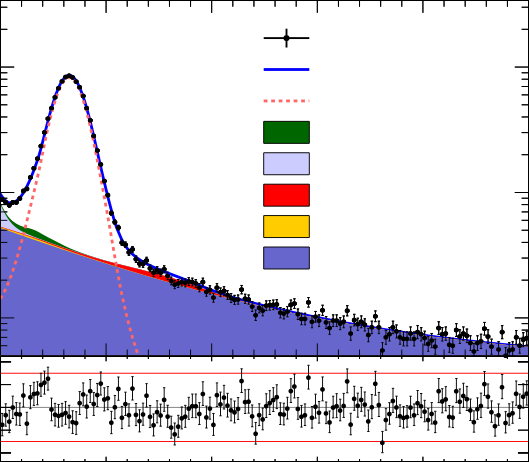
\includegraphics[width=0.9\textwidth]{BsDsK_TD/MDFit_Results/mass_Bs2DsPi_BeautyMass_both_all_run1_nominal}};
            \begin{scope}[x={(image.south east)},y={(image.north west)}]
                \foreach \x/\xtext in {5300, 5400, ..., 5800}
                {
                    \tikzmath{\xpos = (\x - 5300) / (5800 - 5300);}
                    \node at (\xpos, -0.025) {\(\xtext\)};
                }
                \node[anchor=base east] at (0.005, 0.297       ) {\(10^{2}\)};
                \node[anchor=base east] at (0.005, 0.297+1*.272) {\(10^{3}\)};
                \node[anchor=base east] at (0.005, 0.297+2*.272) {\(10^{4}\)};
                \foreach \p in {0, ..., 4}
                {
                    \tikzmath{\ypos = (\p / 4) * 0.198 + .020; \ptext = (\p - 2) * 2;}
                    \node[anchor=east] at (0.005, \ypos) {\(\scriptstyle\pgfmathprintnumber[fixed,precision=0,fixed zerofill=true]{\ptext}\)};
                }
                \node[anchor=east] at (1.0, -0.09) {\({m(\DsmpPipm)}~[\si{\MeVcc}]\)};
                \node[rotate=90,anchor=east,inner xsep=0pt,outer xsep=0pt] at (-0.11, 1.0) {\({\text{Candidates}/(\SI{5.0}{\MeVcc})}\)};
                \node[anchor=west] at (0.06, 0.92) {\Huge\lhcb};
                % Legend
                {
                    \node[anchor=base west] at (0.585, 0.906) {Data};
                    \node[anchor=base west] at (0.585, 0.906 - 1 * 0.0682) {Total fit};
                    \node[anchor=base west] at (0.585, 0.906 - 2 * 0.0682) {\BsDsPi~signal};
                    \node[anchor=base west] at (0.585, 0.906 - 3 * 0.0682) {\BsDsK};
                    \node[anchor=base west] at (0.585, 0.906 - 4 * 0.0682) {\decay{\BorBsz}{\DsorDssm\pip}};
                    \node[anchor=base west] at (0.585, 0.906 - 5 * 0.0682) {\LbLcPi};
                    \node[anchor=base west] at (0.585, 0.906 - 6 * 0.0682) {\BdDPi};
                    \node[anchor=base west] at (0.585, 0.906 - 7 * 0.0682) {Combinatorial};
                }
            \end{scope}
        \end{tikzpicture}
        \caption{\DsmpPipm~invariant mass.}
    \end{subfigure} \par\bigskip
    \begin{subfigure}{.48\textwidth} \centerfloat
        \begin{tikzpicture}
            \node[anchor=south west,inner sep=0] (image) at (0,0) {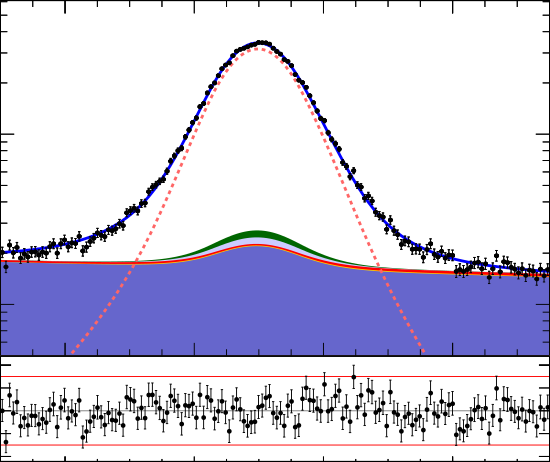
\includegraphics[width=0.9\textwidth]{BsDsK_TD/MDFit_Results/mass_Bs2DsPi_CharmMass_both_all_run1_nominal}};
            \begin{scope}[x={(image.south east)},y={(image.north west)}]
                \fontsize{8}{9.6}\selectfont
                \foreach \x/\xtext in {1940, 1960, ..., 2000}
                {
                    \tikzmath{\xpos = (\x - 1940) / (2000 - 1940) * (0.822 - 0.12) + 0.12;}
                    \node at (\xpos, -0.032) {\(\xtext\)};
                }
                \node[anchor=base east] at (0.005, 0.327) {\(10^{2}\)};
                \node[anchor=base east] at (0.005, 0.694) {\(10^{3}\)};
                \foreach \p in {0, ..., 4}
                {
                    \tikzmath{\ypos = (\p / 4) * 0.198 + .013; \ptext = (\p - 2) * 2;}
                    \node[anchor=east] at (0.005, \ypos) {\(\scriptstyle\pgfmathprintnumber[fixed,precision=0,fixed zerofill=true]{\ptext}\)};
                }
                \node[anchor=east] at (1.0, -0.11) {\({m(\Dsmp)}~[\si{\MeVcc}]\)};
                \node[rotate=90,anchor=east,inner xsep=0pt,outer xsep=0pt] at (-0.13, 1.0) {\({\text{Candidates}/(\SI{0.85}{\MeVcc})}\)};
                \node[anchor=west] at (0.06, 0.92) {\Large\lhcb};
            \end{scope}
        \end{tikzpicture}
        \caption{\Dsmp~invariant mass.}
    \end{subfigure} \hfill%
    \begin{subfigure}{.48\textwidth} \centerfloat
        \begin{tikzpicture}
            \node[anchor=south west,inner sep=0] (image) at (0,0) {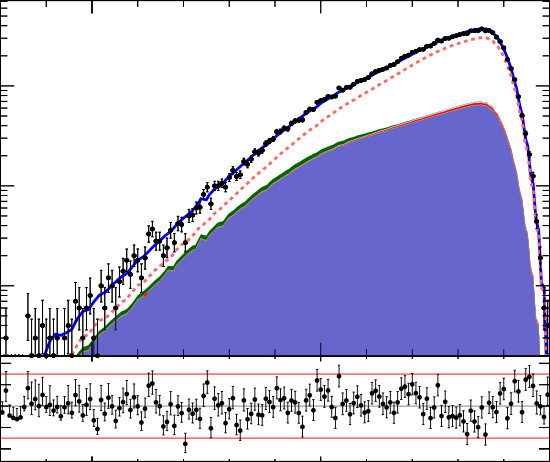
\includegraphics[width=0.9\textwidth]{BsDsK_TD/MDFit_Results/mass_Bs2DsPi_BacPIDK_both_all_run1_nominal}};
            \begin{scope}[x={(image.south east)},y={(image.north west)}]
                \fontsize{8}{9.6}\selectfont
                \node at (0.163, -0.032) {\num{-5}};
                \node at (0.583, -0.032) {\num{ 0}};
                \node at (1.   , -0.032) {\num{ 5}};
                \node[anchor=base east] at (0.005, 0.362       ) {\(10\)};
                \node[anchor=base east] at (0.005, 0.362+1*.217) {\(10^{2}\)};
                \node[anchor=base east] at (0.005, 0.362+2*.217) {\(10^{3}\)};
                \foreach \p in {0, ..., 4}
                {
                    \tikzmath{\ypos = (\p / 4) * 0.198 + .013; \ptext = (\p - 2) * 2;}
                    \node[anchor=east] at (0.005, \ypos) {\(\scriptstyle\pgfmathprintnumber[fixed,precision=0,fixed zerofill=true]{\ptext}\)};
                }
                \node[anchor=east] at (1.0, -0.09) {\({\log(-\dllkpi)}\)};
                \node[rotate=90,anchor=east,inner xsep=0pt,outer xsep=0pt] at (-0.13, 1.0) {\({\text{Candidates}/0.12}\)};
                \node[anchor=west] at (0.06, 0.92) {\large\lhcb};
            \end{scope}
        \end{tikzpicture}
        \caption{Companion~\dllkpi.}
    \end{subfigure}
    \caption{
        Results of the multivariate fit to \BsDsPi~candidates.}
    \label{fig:BsDsK_TD_DsPi_MDFit_Results}
\end{figure}

\begin{landscape}
\begin{table}[p] \centerfloat
    \caption{
        Results of the multivariate fit to the final state~\DsmpKpm.
        The \(N\)~represent yields, and the \DCBmu~are the mean values of the \Bs~and \Dsmp~signal shapes.
        The \(s_{\text{comb}}\)~are the slopes of combinatorial background, in units of~\num{e-3}.
        The fraction~\(f_{\text{comb, \Bs}}\) is the fraction between the exponential and constant components in the \DsmpKpm~mass, whereas \(f_{\text{comb, \Dsmp}}\)~represents the fraction between the combinatorial exponential and DCB~shapes in the \Dsmp~mass.
        The \(f_{\text{comb, \dll}}\)~are the fractions between the components in the \dllkpi~combinatorial shape: \(f_{\text{comb, \dll,1}}\)~is the fraction of pions and \({(1 - f_{\text{comb, \dll,1}}) f_{\text{comb, \dll,2}}}\)~corresponds to the fraction of kaons.
        Finally, \(f_{\BsDsPi}\)~is the fraction between \BsDsPi~and the partially reconstructed backgrounds, and \(f_{\Lb}\)~is the fraction between all backgrounds of the form~\BsDsOrDsstPi and the sum of the two backgrounds~\LbDsOrDsstp.}
    \label{tab:BsDsK_TD_DsK_MDFit_Results}
    \begin{tabular}{lccccc}
        \toprule
        Parameter & \DsmNonRes & \DsmPhiPi & \DsmKstK & \DsmKPiPi & \DsmPiPiPi \tabularnewline
        \midrule
        \(N_{\BsDsK}\)              & \err{1055}{38}   & \err{1957}{51}   & \err{1616}{46}   & \err{\0391}{24}      & \err{\0936}{37} \tabularnewline
        \midrule
        \(N_{\BdDsK}\)              & \err{\0\032}{10} & \err{\0\049}{13} & \err{\0\050}{12} & \err{\0\024}{\07} & \err{\0\041}{11} \tabularnewline[.3ex]
        \rowcolor{tableshade}
        \(N_{\text{backgrounds}}\)  & \err{\0676}{36} & \err{1513}{57} & \err{1062}{50} & \err{\0208}{23} & \err{\0763}{43} \tabularnewline[.3ex]
        \(N_{\text{comb}}\)         & \err{1370}{47} & \err{\0736}{55} & \err{\0707}{53} & \err{1113}{40} & \err{2173}{59} \tabularnewline[.3ex]
        \midrule
        \(\DCBmu_{\Bs}\)~(\si{\MeVcc})   & \multicolumn{5}{c}{\raisebox{.5ex}{\rule{.33\linewidth}{.3pt}}~\err{5365.2}{0.2}~\raisebox{.5ex}{\rule{.33\linewidth}{.3pt}}} \tabularnewline[.3ex]
        \rowcolor{tableshade}
        \(\DCBmu_{\Dsmp}\)~(\si{\MeVcc}) & \multicolumn{5}{c}{\raisebox{.5ex}{\rule{.33\linewidth}{.3pt}}~\err{1969.7}{0.1}~\raisebox{.5ex}{\rule{.33\linewidth}{.3pt}}} \tabularnewline[.3ex]
        \midrule
        \(s_{\text{comb, \Bs}} \times \num{e3}\)   & \err{-6.8\0}{1.0\0} & \err{-12.2}{0.9\0}  & \err{-7.9\0}{1.5\0} & \err{-1.40}{0.24}   & \err{-1.63}{0.18} \tabularnewline[.3ex]
        \rowcolor{tableshade}
        \(f_{\text{comb, \Bs}}\)    & \err{\n0.64}{0.07} & \err{\n0.37}{0.05} & \err{\n0.63}{0.08} & -- & -- \tabularnewline[.3ex]
        \(s_{\text{comb, \Dsmp}} \times \num{e3}\) & \err{-0.4\0}{0.1\0} & \err{-7.6\0}{2.1\0} & \err{-1.6\0}{1.9\0} & \err{-1.0\0}{1.2\0} & \err{-3.8\0}{0.9\0} \tabularnewline[.3ex]
        \rowcolor{tableshade}
        \(f_{\text{comb, \Dsmp}}\)  & \err{\n0.99}{0.09} & \err{\n0.61}{0.05} & \err{\n0.72}{0.05} & \err{\n1.00}{0.07} & \err{\n1.00}{0.02} \tabularnewline[.3ex]
        \(f_{\text{comb, \dll,1}}\) & \err{\n0.28}{0.04} & \err{\n0.12}{0.07} & \err{\n0.31}{0.07} & \err{\n0.01}{0.04} & \err{\n0.15}{0.03} \tabularnewline
        \rowcolor{tableshade}
        \(f_{\text{comb, \dll,2}}\) & \err{\n0.77}{0.08} & \err{\n0.55}{0.09} & \err{\n0.93}{0.16} & \err{\n0.66}{0.07} & \err{\n0.60}{0.05} \tabularnewline
        \midrule
        \(f_{\BsDsPi}\)             & \multicolumn{5}{c}{\raisebox{.5ex}{\rule{.33\linewidth}{.3pt}}~\err{0.729}{0.021}~\raisebox{.5ex}{\rule{.33\linewidth}{.3pt}}} \tabularnewline
        \rowcolor{tableshade}
        \(f_{\Lb}\)                 & \multicolumn{5}{c}{\raisebox{.5ex}{\rule{.33\linewidth}{.3pt}}~\err{0.923}{0.023}~\raisebox{.5ex}{\rule{.33\linewidth}{.3pt}}} \tabularnewline
        \bottomrule
     \end{tabular}
\end{table}
\end{landscape}

\begin{figure}[hp] \centerfloat
    \begin{subfigure}{\textwidth} \centerfloat
        \begin{tikzpicture}
            \node[anchor=south west,inner sep=0] (image) at (0,0) {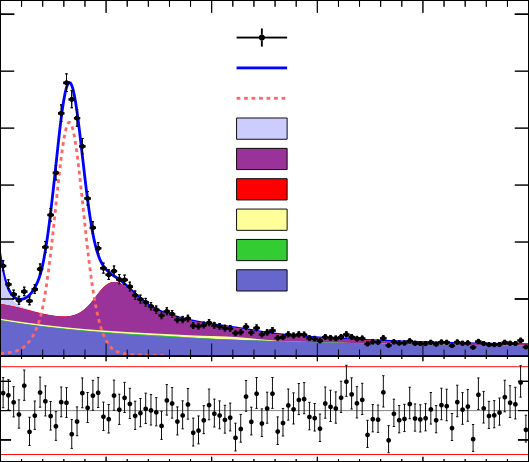
\includegraphics[width=0.9\textwidth]{BsDsK_TD/MDFit_Results/mass_Bs2DsK_BeautyMass_both_all_run1_nominal}};
            \begin{scope}[x={(image.south east)},y={(image.north west)}]
                \foreach \x/\xtext in {5300, 5400, ..., 5800}
                {
                    \tikzmath{\xpos = (\x - 5300) / (5800 - 5300);}
                    \node at (\xpos, -0.025) {\(\xtext\)};
                }
                \foreach \y in {0, ..., 6}
                {
                    \tikzmath{\ypos = (\y / 6) * 0.740 + 0.217; \ytext = 200 * \y;}
                    \node[anchor=base east] at (0.005, \ypos) {\(\pgfmathprintnumber[fixed,precision=0,fixed zerofill=true,1000 sep={}]{\ytext}\)};
                }
                \foreach \p in {0, ..., 2}
                {
                    \tikzmath{\ypos = (\p / 2) * 0.127 + .048; \ptext = (\p - 1) * 2;}
                    \node[anchor=east] at (0.005, \ypos) {\(\scriptstyle\pgfmathprintnumber[fixed,precision=0,fixed zerofill=true]{\ptext}\)};
                }
                \node[anchor=east] at (1.0, -0.09) {\({m(\DsmpKpm)}~[\si{\MeVcc}]\)};
                \node[rotate=90,anchor=east,inner xsep=0pt,outer xsep=0pt] at (-0.11, 1.0) {\({\text{Candidates}/(\SI{5.0}{\MeVcc})}\)};
                \node[anchor=west] at (0.06, 0.92) {\Huge\lhcb};
                % Legend
                {
                    \node[anchor=base west] at (0.55, 0.906) {Data};
                    \node[anchor=base west] at (0.55, 0.906 - 1 * 0.0656) {Total fit};
                    \node[anchor=base west] at (0.55, 0.906 - 2 * 0.0656) {\BsDsK~signal};
                    \node[anchor=base west] at (0.55, 0.906 - 3 * 0.0656) {\decay{\BorBsz}{\DsorDssmp\KorKstpm}};
                    \node[anchor=base west] at (0.55, 0.906 - 4 * 0.0656) {\decay{\Bs}{\DsorDssm(\pip, \rhop)}};
                    \node[anchor=base west] at (0.55, 0.906 - 5 * 0.0656) {\decay{\Bd}{\Dm(\pip, \Kp)}};
                    \node[anchor=base west] at (0.55, 0.906 - 6 * 0.0656) {\LbDsOrDsstp};
                    \node[anchor=base west] at (0.55, 0.906 - 7 * 0.0656) {\decay{\Lb}{\Lcp(\pim, \Km)}};
                    \node[anchor=base west] at (0.55, 0.906 - 8 * 0.0656) {Combinatorial};
                }
            \end{scope}
        \end{tikzpicture}
        \caption{\DsmpKpm~invariant mass.}
    \end{subfigure} \par\bigskip
    \begin{subfigure}{.48\textwidth} \centerfloat
        \begin{tikzpicture}
            \node[anchor=south west,inner sep=0] (image) at (0,0) {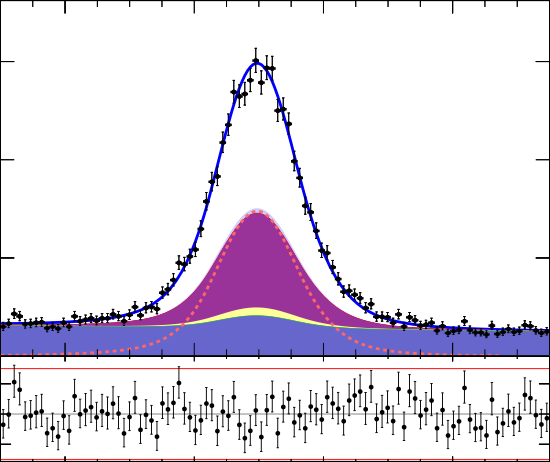
\includegraphics[width=0.9\textwidth]{BsDsK_TD/MDFit_Results/mass_Bs2DsK_CharmMass_both_all_run1_nominal}};
            \begin{scope}[x={(image.south east)},y={(image.north west)}]
                \fontsize{8}{9.6}\selectfont
                \foreach \x/\xtext in {1940, 1960, ..., 2000}
                {
                    \tikzmath{\xpos = (\x - 1940) / (2000 - 1940) * (0.822 - 0.12) + 0.12;}
                    \node at (\xpos, -0.032) {\(\xtext\)};
                }
                \foreach \y in {0, ..., 3}
                {
                    \tikzmath{\ypos = (\y / 3) * 0.640 + 0.21; \ytext = 200 * \y;}
                    \node[anchor=base east] at (0.005, \ypos) {\(\pgfmathprintnumber[fixed,precision=0,fixed zerofill=true]{\ytext}\)};
                }
                \foreach \p in {0, ..., 2}
                {
                    \tikzmath{\ypos = (\p / 2) * 0.127 + .044; \ptext = (\p - 1) * 2;}
                    \node[anchor=east] at (0.005, \ypos) {\(\scriptstyle\pgfmathprintnumber[fixed,precision=0,fixed zerofill=true]{\ptext}\)};
                }
                \node[anchor=east] at (1.0, -0.11) {\({m(\Dsmp)}~[\si{\MeVcc}]\)};
                \node[rotate=90,anchor=east,inner xsep=0pt,outer xsep=0pt] at (-0.13, 1.0) {\({\text{Candidates}/(\SI{0.85}{\MeVcc})}\)};
                \node[anchor=west] at (0.06, 0.92) {\Large\lhcb};
            \end{scope}
        \end{tikzpicture}
        \caption{\Dsmp~invariant mass.}
    \end{subfigure} \hfill%
    \begin{subfigure}{.48\textwidth} \centerfloat
        \begin{tikzpicture}
            \node[anchor=south west,inner sep=0] (image) at (0,0) {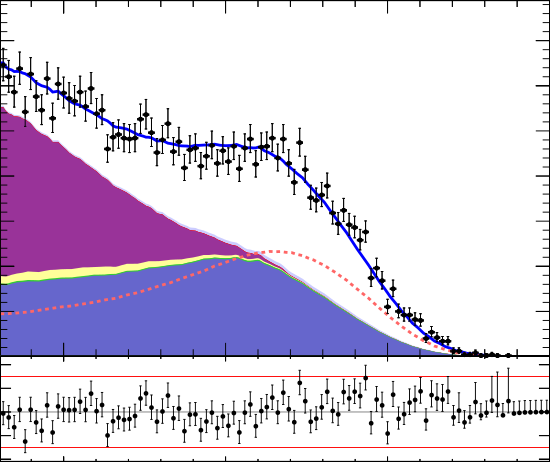
\includegraphics[width=0.9\textwidth]{BsDsK_TD/MDFit_Results/mass_Bs2DsK_BacPIDK_both_all_run1_nominal}};
            \begin{scope}[x={(image.south east)},y={(image.north west)}]
                \fontsize{8}{9.6}\selectfont
                \foreach \x/\xtext in {0, ..., 3}
                {
                    \tikzmath{\xpos = (\x / 3) * 0.883 + 0.117; \xtext = \x + 2;}
                    \node at (\xpos, -0.032) {\pgfmathprintnumber[fixed,precision=0,fixed zerofill=true]{\xtext}};
                }
                \foreach \y in {1, ..., 7}
                {
                    \tikzmath{\ypos = (\y / 7) * 0.682 + 0.210; \ytext = 50 * \y;}
                    \node[anchor=base east] at (0.005, \ypos) {\(\pgfmathprintnumber[fixed,precision=0,fixed zerofill=true]{\ytext}\)};
                }
                \foreach \p in {0, ..., 4}
                {
                    \tikzmath{\ypos = (\p / 4) * 0.205 + .007; \ptext = (\p - 2) * 2;}
                    \node[anchor=east] at (0.005, \ypos) {\(\scriptstyle\pgfmathprintnumber[fixed,precision=0,fixed zerofill=true]{\ptext}\)};
                }
                \node[anchor=east] at (1.0, -0.09) {\({\log(\dllkpi)}\)};
                \node[rotate=90,anchor=east,inner xsep=0pt,outer xsep=0pt] at (-0.13, 1.0) {\({\text{Candidates}/0.03}\)};
                \node[anchor=west] at (0.70, 0.92) {\large\lhcb};
            \end{scope}
        \end{tikzpicture}
        \caption{Companion~\dllkpi.}
    \end{subfigure}
    \caption{
        Results of the multivariate fit to \BsDsK~candidates.}
    \label{fig:BsDsK_TD_DsK_MDFit_Results}
\end{figure}

\clearpage
\subsection{Fit validation}
\label{sec:BsDsK_TD_MDFit_Validation}

The multivariate fit procedure is validated by applying it to several subsamples, repeating the entire procedure described in this \lcnamecref{sec:BsDsK_TD_MDFit_Validation}
The data is split by:
%
\begin{enumerate}
    \item \lhcb~magnet polarity;
    \item centre-of-mass energy;
    \item BDT~response;
    \item \Bs~momentum, split at~\SI{120}{\GeVc}.
\end{enumerate}
%
In the latter two cases, the split value is chosen such that the remaining samples have roughly the same signal yields in simulation.
To check the results of the splits, the sum of the signal yields of the split fits are compared with the signal yield of the fit on the full data set.
These yields are shown in \cref{tab:BsDsK_TD_MDFit_Split}.
The individual fits each have good quality, and the yields also show good agreement.
To further validate these splits, the decay-time fit is also performed separately on the partial data samples (see \cref{sec:BsDsK_TD_Syst}).
%
\begin{table}[htb] \centerfloat
    \caption{
        Total yields of the full and split data sample, resulting from the respective multivariate fits.}
    \label{tab:BsDsK_TD_MDFit_Split}
    \rowcolors{1}{tableshade}{}
    \begin{tabular}{lS[table-format=5(3)]S[table-format=4(2)]}
        \hiderowcolors \toprule
        \multirow{2}{*}[-2pt]{Sample} & \multicolumn{2}{c}{Total yield} \tabularnewline
        \cmidrule(lr){2-3}
                    & {\BsDsPi}    & {\BsDsK} \tabularnewline
        \showrowcolors \midrule
        Full sample & 96942 +- 345 & 5955 +- 90 \tabularnewline
        Split 1     & 96985 +- 345 & 5962 +- 91 \tabularnewline
        Split 2     & 97010 +- 345 & 5953 +- 90 \tabularnewline
        Split 3     & 96334 +- 342 & 5873 +- 90 \tabularnewline
        Split 4     & 97170 +- 346 & 5911 +- 95 \tabularnewline
        \bottomrule
    \end{tabular}
\end{table}

\clearpage

\setchapterpreamble{
    \lettrine{T}{his}~\lcnamecref{chp:BsDsK_TD} discusses the decay-time fit to the \BsDsK~sample obtained in \cref{chp:BsDsK_TD_Data}.
    This fit yields five \CP-violation parameters, \Cpar, \Spar, \Sbpar, \Dpar, and~\Dbpar, from which the CKM~parameter \CPgamma~is subsequently extracted.}
\chapter[\CP~violation in \BsDsK]{Time-dependent measurement of \CP~violation in~\BsDsK}
\label{chp:BsDsK_TD}

\vspace*{\fill}
\minitoc

\clearpage
\section{Decay-time resolution} \label{sec:BsDsK_TD_Res}

The oscillation period of the \Bs~system is of the same order of magnitude as the time resolution of the detector, which implies that the decay-time distribution of the \Bs~candidates is significantly diluted by the resolution.
This is accounted for in the decay-time fit, and in order to do so, the resolution is determined for each event.

The decay time~\(t\) is determined by a fit to the position of the \Bs~decay vertex~\(\vec{x}_\text{SV}\), its reconstructed momentum vector \(\vec{\ptot}\), and its proper decay time~\(t\), using the constraint
%
\begin{equation}
    \vec{x}_{\text{SV}} - \vec{x}_{\text{PV}} = t \dfrac{\vec{\ptot}}{m_{\Bs}} \rlap{,}
\end{equation}
%
where the position of the~PV~\(\vec{x}_{\text{PV}}\) is fixed by other tracks in the event and \(m_{\Bs}\)~is the known mass of the \Bs~meson~\cite{PDG}.
By excluding the four tracks from which the~SV is reconstructed from the PV~reconstruction, the correlation between~\(\vec{x}_{\text{PV}}\) and the other variables is nullified.

Input to this fit are the reconstructed tracks of the four decay particles~(\({\decay{\Bs}{\Dsmp(\to\KmpKPi)\Kpm}}\)) and their covariances resulting from the known detector resolution, multiple scattering, and kinematics.
As a result, both the decay time~\(t\) and the error on the decay time~\(\dt\) can be determined.
This error is called the per-event decay-time error throughout this \lcnamecref{sec:BsDsK_TD_Res}.
The error on the PV~location is negligible compared to that on the SV~location, and the correlation between \(\vec{x}_{\text{PV}}\)~and \(\vec{\ptot}\)~is small because of the way these variables are determined from track fits.
Consequently, \(\dt\)~is dominated by the errors on the SV~reconstruction and momentum determination, which in turn are dominated by the hit resolution in the tracking stations and the amount of detector material traversed.

\subsection{Decay-time error calibration} \label{sec:BsDsK_TD_Res_Calib}
The reconstructed per-event decay-time error provides a measure for the underlying resolution.
However, it is found that the per-event decay-time error somewhat underestimates the actual decay-time resolution, and thus must be calibrated before it can be used as input to the fit.
This calibration is done by using a sample of prompt \Dspm~candidates (\DspmKKPi) from data, and combining each candidate with a random track (again labelled as companion track) also originating from the~PV (see \cref{fig:BsDsK_TD_Res_Topology}).
The combination of these four tracks has kinematics similar to those of the signal process, except that the true decay time of each of these events is now known to be~\num{0}.
By reconstructing the decay time and taking the difference with~\num{0}, the resolution is obtained.
To reject possible contributions from real \Bs~mesons in this calibration procedure, the resolution is determined from events with a negative reconstructed decay time.
The decay-time resolution is determined for the final state~\DspmKKPi.
The difference in decay-time resolution for the other modes is smaller than~\SI{2}{\percent} as obtained from simulation, and is ignored.

\begin{figure}[htb] \centerfloat
    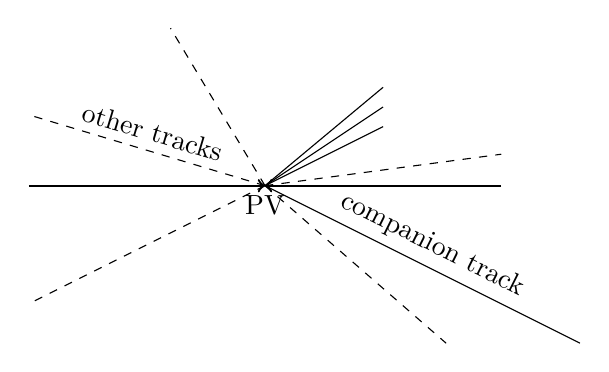
\begin{tikzpicture}[font=\captionfont]
        \coordinate (PV) at (0, 0);
        \coordinate (p1) at (-3, 0);
        \coordinate (p2) at (3, 0);
        \coordinate (comp) at (4, -2);
        \coordinate (h1) at (1.5, 1.25);
        \coordinate (h2) at (1.5, 1);
        \coordinate (h3) at (1.5, 0.75);

        \draw [thick,->] (p1) -- (PV) node [at start,anchor=north west] {\normalsize \proton} node [at end,anchor=north] {PV};
        \draw [thick,->] (p2) -- (PV) node [at start,anchor=north east] {\normalsize \proton};
        \draw (PV) -- (comp) node [midway,above=-0.075,sloped] {companion track};
        \draw (PV) -- (h1) node [midway,above,sloped] {\Dspm};
        \draw (PV) -- (h2) node {};
        \draw (PV) -- (h3) node {};

        \draw [dashed] (PV) -- (-1.2,  2);
        \draw [dashed] (PV) -- ( 2.3, -2);
        \draw [dashed] (PV) -- ( 3,    0.4);
        \draw [dashed] (PV) -- (-3,    0.9) node [midway,above,sloped] {other tracks};
        \draw [dashed] (PV) -- (-3,   -1.5);
    \end{tikzpicture}
    \caption{
        Decay topology of prompt \Dspm~candidates combined with a random track, which are used to calibrate the decay-time resolution.}
    \label{fig:BsDsK_TD_Res_Topology}
\end{figure}

The prompt \Dspm~sample and companion tracks are selected according to the same procedure as specified in \cref{sec:stripping}, except that some constraints are relaxed.
The companion track is not required to have a minimal~\chisqip, and the combination of \Dspm~candidate and companion track is not required to have a minimal displacement from the~PV, or to point back at it.
Loosening these requirements is necessary to produce a decay-time unbiased sample.
Some additional constraints are applied: the number of reconstructed~PVs is required to be~\num{1}, the flight-distance~\chisq of the \Dspm~combination with respect to the~PV is required to be~\({< \num{2}}\), and the companion track \dllmupi~to be \({< \num{2}}\).

To obtain a signal sample, combinatorial \Dspm~combinations are statistically subtracted from the sample using the \sfit~method~\cite{Yuehong_sFit}, by performing a fit to the \KKPi~invariant mass.
The \Dspm~component of this fit is defined as a double Crystal~Ball~(DCB) shape with common mean~\DCBmu and width~\DCBs, and the combinatorial background is parameterised as an exponential.
The results of the fit are shown in \cref{tab:BsDsK_TD_Res_sFit_Results,fig:BsDsK_TD_Res_sFit_Results}.
%
\begin{table}[htb] \centerfloat
    \caption{
        Result of the fit to the \KKPi~invariant mass of the prompt sample.
        Values quoted without an error are fixed in the fit.}
    \label{tab:BsDsK_TD_Res_sFit_Results}
    \rowcolors{2}{tableshade}{}
    \sisetup{table-number-alignment=right}
    \begin{tabular}{lS[table-format=6.3(3)]}
        \toprule
        Parameter & {Fitted value}\tabularnewline
        \midrule
        \(N_{\text{prompt~\Dspm}}\)  & 101882     +- 1635 \tabularnewline
        \(N_{\text{combinatorial}}\) & 563671     +- 2677 \tabularnewline
        \DCBmu~(\si{\MeVcc})         &   1969.80  +-    0.01  \tabularnewline
        \DCBs~(\si{\MeVcc})          &      6.220 +-    0.012 \tabularnewline
        \midrule
        \DCBaL & -1.24 \tabularnewline
        \DCBaR &  1.34 \tabularnewline
        \DCBnL &  6.67 \tabularnewline
        \DCBnR &  3.43 \tabularnewline
        \DCBf  &  0.5  \tabularnewline
        \bottomrule
    \end{tabular}
\end{table}
%
\begin{figure}[htb] \centerfloat
    \begin{tikzpicture}
        \node[anchor=south west,inner sep=0] (image) at (0,0) {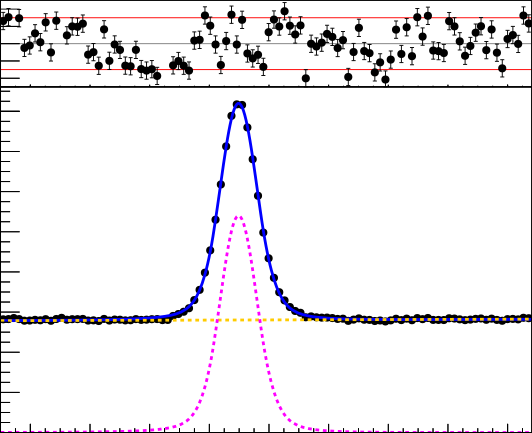
\includegraphics[width=0.9\textwidth]{BsDsK_TD/Time_Resolution/Mfit_ALL}};
        \begin{scope}[x={(image.south east)},y={(image.north west)}]
            \foreach \x in {0, ..., 8}
            {
                \tikzmath{\xpos = (\x / 8) * 0.896 + 0.058; \xtext = 20 * \x + 1900;}
                \node at (\xpos, -0.025) {\(\pgfmathprintnumber[fixed,precision=0,fixed zerofill=true,1000 sep={}]{\xtext}\)};
            }
            \foreach \y in {0, ..., 8}
            {
                \tikzmath{\ypos = (\y / 8) * 0.743; \ytext = 20 * \y;}
                \node[anchor=east] at (0.005, \ypos) {\(\pgfmathprintnumber[fixed,precision=0,fixed zerofill=true]{\ytext}\)};
            }
            \foreach \p in {0, ..., 4}
            {
                \tikzmath{\ypos = (\p / 4) * 0.159 + 0.819; \ptext = (\p - 2) * 2;}
                \node[anchor=east] at (0.005, \ypos) {\(\scriptstyle\pgfmathprintnumber[fixed,precision=0,fixed zerofill=true]{\ptext}\)};
            }
            \node[anchor=south] at (0.03, 1.) {\({\times \num{e2}}\)};
            \node[anchor=east] at (1.0, -0.09) {\({m(\Dspm)}~[\si{\MeVcc}]\)};
            \node[rotate=90,anchor=east,inner xsep=0pt,outer xsep=0pt] at (-0.10, 1.0) {\({\text{Candidates}/(\SI{1.78}{\MeVcc})}\)};
            \node[anchor=west] at (0.06, 0.72) {\Large\lhcb};
        \end{scope}
    \end{tikzpicture}
    \caption{
        Result of the fit to the \KKPi~invariant mass of the prompt sample.}
    \label{fig:BsDsK_TD_Res_sFit_Results}
\end{figure}

From the resulting, statistically pure \Dspm~sample, the resolution of the combination of \Dspm~and random companion track is determined.
The sample is binned in bins of reconstructed per-event decay-time error \dt~(see \cref{tab:BsDsK_TD_Res_Nominal}), and in each bin a double Gaussian shape is effectively fitted to the negative tail of the reconstructed decay time.
The fit takes into account a small range of positive decay-time events in order to correctly model the shape.
The fit model is the sum of two Gaussian functions, where the main part is a narrow Gaussian that accounts for well-measured events and a smaller part is a wider Gaussian for those with a larger uncertainty.
Two example fits are shown in \cref{fig:BsDsK_TD_Res_GaussianFits}.
%
\begin{figure}[hp] \centerfloat
    \fontsize{9}{10.8}\selectfont
    \begin{subfigure}{.8\textwidth} \centerfloat
        \begin{tikzpicture}
            \node[anchor=south west,inner sep=0] (image) at (0,0) {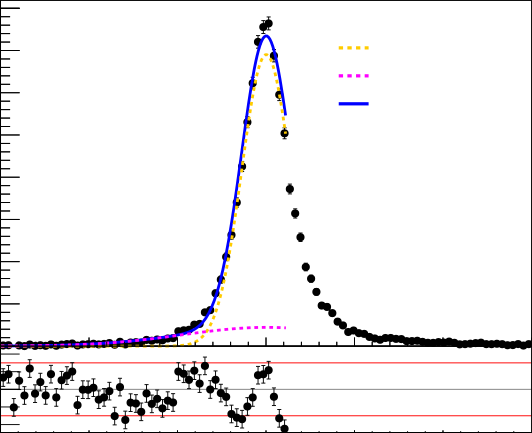
\includegraphics[width=0.9\textwidth]{BsDsK_TD/Time_Resolution/bin002}};
            \begin{scope}[x={(image.south east)},y={(image.north west)}]
                \foreach \x in {0, ..., 6}
                {
                    \tikzmath{\xpos = (\x / 6); \xtext = 100 * \x - 300;}
                    \node at (\xpos, -0.025) {\(\pgfmathprintnumber[fixed,precision=0,fixed zerofill=true]{\xtext}\)};
                }
                \node[anchor=east] at (0.005, .215) {\(0\)};
                \foreach \y in {1, ..., 8}
                {
                    \tikzmath{\ypos = (\y / 8) * 0.777 + .203; \ytext = 500 * \y;}
                    \node[anchor=east] at (0.005, \ypos) {\(\pgfmathprintnumber[fixed,precision=0,fixed zerofill=true,1000 sep={}]{\ytext}\)};
                }
                \foreach \p in {0, ..., 4}
                {
                    \tikzmath{\ypos = (\p / 4) * 0.163 + .02; \ptext = (\p - 2) * 2;}
                    \node[anchor=east] at (0.005, \ypos) {\(\scriptstyle\pgfmathprintnumber[fixed,precision=0,fixed zerofill=true]{\ptext}\)};
                }
                % Legend
                {
                    \node[anchor=base west] at (0.70, 0.876) {Narrow Gaussian};
                    \node[anchor=base west] at (0.70, 0.812) {Wide Gaussian};
                    \node[anchor=base west] at (0.70, 0.748) {Total};
                }
                \node[anchor=east] at (1.0, -0.09) {Decay time~\([\si{\fs}]\)};
                \node[rotate=90,anchor=east,inner xsep=0pt,outer xsep=0pt] at (-0.12, 1.0) {\({\text{Candidates}/(\SI{6.0}{\fs})}\)};
                \node[anchor=west] at (0.06, 0.92) {\Large\lhcb};
            \end{scope}
        \end{tikzpicture}
        \caption{\({\SI{20}{\fs} < \dt < \SI{25}{\fs}}\).}
        \label{fig:BsDsK_TD_Res_GaussianFits_Low}
    \end{subfigure}
    \par\bigskip
    \begin{subfigure}{.8\textwidth} \centerfloat
        \begin{tikzpicture}
            \node[anchor=south west,inner sep=0] (image) at (0,0) {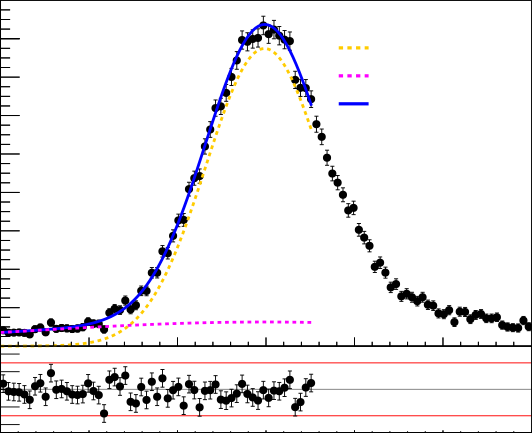
\includegraphics[width=0.9\textwidth]{BsDsK_TD/Time_Resolution/bin017}};
            \begin{scope}[x={(image.south east)},y={(image.north west)}]
                \foreach \x in {0, ..., 6}
                {
                    \tikzmath{\xpos = (\x / 6); \xtext = 100 * \x - 300;}
                    \node at (\xpos, -0.025) {\(\pgfmathprintnumber[fixed,precision=0,fixed zerofill=true]{\xtext}\)};
                }
                \node[anchor=east] at (0.005, .215) {\(0\)};
                \foreach \y in {1, ..., 8}
                {
                    \tikzmath{\ypos = (\y / 8) * 0.708 + .203; \ytext = 200 * \y;}
                    \node[anchor=east] at (0.005, \ypos) {\(\pgfmathprintnumber[fixed,precision=0,fixed zerofill=true,1000 sep={}]{\ytext}\)};
                }
                \foreach \p in {0, ..., 4}
                {
                    \tikzmath{\ypos = (\p / 4) * 0.163 + .02; \ptext = (\p - 2) * 2;}
                    \node[anchor=east] at (0.005, \ypos) {\(\scriptstyle\pgfmathprintnumber[fixed,precision=0,fixed zerofill=true]{\ptext}\)};
                }
                % Legend
                {
                    \node[anchor=base west] at (0.70, 0.876) {Narrow Gaussian};
                    \node[anchor=base west] at (0.70, 0.812) {Wide Gaussian};
                    \node[anchor=base west] at (0.70, 0.748) {Total};
                }
                \node[anchor=east] at (1.0, -0.09) {Decay time~\([\si{\fs}]\)};
                \node[rotate=90,anchor=east,inner xsep=0pt,outer xsep=0pt] at (-0.12, 1.0) {\({\text{Candidates}/(\SI{6.0}{\fs})}\)};
                \node[anchor=west] at (0.06, 0.92) {\Large\lhcb};
            \end{scope}
        \end{tikzpicture}
        \caption{\({\SI{50}{\fs} < \dt \SI{55}{\fs}}\).}
        \label{fig:BsDsK_TD_Res_GaussianFits_High}
    \end{subfigure}
    \caption{
        Fits to the reconstructed decay time of prompt~\Dspm-random track combinations, for two \dt~bins.
        As expected, the lower \dt~bin in~(\subref{fig:BsDsK_TD_Res_GaussianFits_Low}) has a narrower decay-time distribution than the higher bin in~(\subref{fig:BsDsK_TD_Res_GaussianFits_High}).}
    \label{fig:BsDsK_TD_Res_GaussianFits}
\end{figure}

In the decay-time fits later on, a single~Gaussian will be used as resolution model, and therefore the widths of these two Gaussian distributions found here are combined into a single, effective resolution.
To do so, the effect of the resolution on the decay-time distribution of an oscillating \Bs~sample is taken into account.
This effect is characterised by a dilution factor~\(D\), as defined in Ref.~\cite{Moser:1996xf}, which depends on the \Bs~oscillation frequency~\dms.
In case of a double-Gaussian resolution model, the dilution becomes
%
\begin{equation} \label{eqn:BsDsK_TD_Res_Dilution}
    D = f_{1} e^{-\sigma_1^{2} \dmssq / 2} + (1 - f_{1}) e^{-\sigma_{2}^{2} \dmssq / 2} \rlap{,}
\end{equation}
%
where the~\(\sigma_{1,2}\) are the widths of the two Gaussian distributions, and \(f_{1}\)~is the relative fraction of the one corresponding to~\(\sigma_{1}\).
The numerical value of this dimensionless quantity runs between~\num{0}, indicating an infinitely poor decay-time resolution, and~\num{1}, indicating that the resolution has infinite precision.
The inverse of \cref{eqn:BsDsK_TD_Res_Dilution} is used to convert the two resolutions back to a single resolution:
%
\begin{equation} \label{eqn:BsDsK_TD_Res_EffectiveSigma}
    \seff = \sqrt{\dfrac{-2}{\dmssq} \log(D)} \rlap{.}
\end{equation}

It should be noted that this \emph{effective}~resolution is not the actual resolution of the \Bs~sample, but rather a resolution of a single Gaussian that has the same dampening effect on the decay-time distribution as the resolution of a double Gaussian would have.
As such, it can be used in the extraction of the \CP-violation parameters.

The resulting distribution of effective resolutions obtained with the prompts~\Dspm method as a function of per-event decay-time error is shown in \cref{fig:BsDsK_TD_Res_Nominal}, and the used binning scheme and result per bin in \cref{tab:BsDsK_TD_Res_Nominal}.To obtain a continuous dependence on the per-event error, it is parameterised using a linear function, resulting in the following expression:
%
\begin{equation} \label{eqn:BsDsK_TD_Res_Nominal}
    \sigma = s_{0} + s_{1} (\dt - \SI{40}{\fs}) = \SI{61.450 +- 0.380}{\fs} + (\num{1.280 +- 0.042}) (\dt - \SI{40}{\fs}) \rlap{,}
\end{equation}
%
where \(s_{0}\)~and \(s_{1}\)~are the linear parameters and \SI{40}{\fs}~is approximately the average per-event decay-time error in real \BsDsK~events.

\begin{figure}[!htb] \centerfloat
    \begin{tikzpicture}
        \node[anchor=south west,inner sep=0] (image) at (0,0) {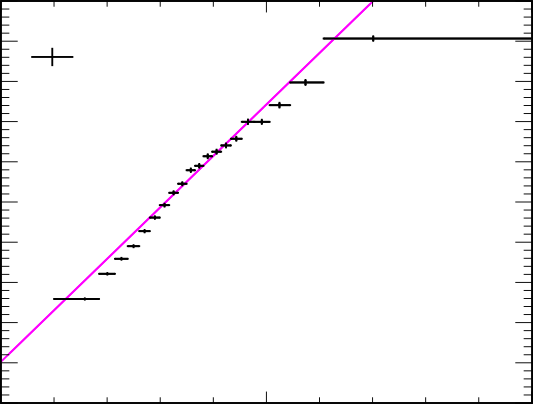
\includegraphics[width=0.9\textwidth]{BsDsK_TD/Time_Resolution/CombinationLinear_ALL_eff_sigma}};
        \begin{scope}[x={(image.south east)},y={(image.north west)}]
            \foreach \x in {0, ..., 10}
            {
                \tikzmath{\xpos = (\x / 10); \xtext = 10 * \x;}
                \node at (\xpos, -0.025) {\(\pgfmathprintnumber[fixed,precision=0,fixed zerofill=true]{\xtext}\)};
            }
            \foreach \y in {0, ..., 10}
            {
                \tikzmath{\ypos = (\y / 10); \ytext = 10 * \y;}
                \node[anchor=east] at (0.005, \ypos) {\(\pgfmathprintnumber[fixed,precision=0,fixed zerofill=true]{\ytext}\)};
            }
            % Legend
            {
                \node[anchor=base west] at (0.14, 0.843) {Prompt~\Dspm data};
                \node[anchor=base west] at (0.14, 0.768) {\BsDsK~data};
            }
            \node[anchor=east] at (1.0, -0.09) {Per-event decay-time error~\dt~\([\si{\fs}]\)};
            \node[rotate=90,anchor=east,inner xsep=0pt,outer xsep=0pt] at (-0.12, 1.0) {Decay-time resolution~\({\sigma~[\si{\fs}]}\)};
            \node[anchor=west] at (0.06, 0.92) {\Large\lhcb};
        \end{scope}
    \end{tikzpicture}
    \caption{
        Measured resolution in bins of the per-event decay-time error (data points) and results of the fit according to the expression in \cref{eqn:BsDsK_TD_Res_Nominal} (solid line).
        The histogram shows the distribution of per-event errors of the \BsDsK~sample with weights from the multivariate fit applied.
        The dashed lines are the relations used to evaluate systematic effects (see \cref{sec:BsDsK_TD_Res_Syst}).}
    \label{fig:BsDsK_TD_Res_Nominal}
\end{figure}
%
\begin{table}[!htb] \centerfloat
    \caption{
        Measured resolution in bins of the per-event decay-time error.}
    \label{tab:BsDsK_TD_Res_Nominal}
    \hspace*{-.75cm}
    \rowcolors{3}{tableshade}{}
    \sisetup{table-number-alignment=right}
    \begin{tabular}{cS[table-format=2.1(1)]cS[table-format=1.2(2)]S[table-format=1.2(1)]S[table-format=2.1(1)]}
        \hiderowcolors \toprule
        \multirow{2}{*}[-2pt]{\dt~bin~(\si{\fs})} & \multicolumn{5}{c}{Double-Gaussian fit results} \tabularnewline
        \cmidrule(lr){2-6}
                             & {\(\sigma_{1}\)~(\si{\fs})} & \(\sigma_{2}\)~(\si{\fs}) & {\(f\)} & {\(D\)} & {\(\seff\)~(\si{\fs})} \tabularnewline
        \showrowcolors \midrule
        \(\09.2\,-\,\018.5\) & 18.1 +- 0.0 & \(\076\,\pm\,\01\) & 0.85 +- 0.0 & 0.86 +- 0.0 & 29.8 +- 0.1 \tabularnewline
        \( 18.5\,-\,\021.5\) & 24.2 +- 0.3 & \(\089\,\pm\,\02\) & 0.85 +- 0.0 & 0.82 +- 0.0 & 35.0 +- 0.2 \tabularnewline
        \( 21.5\,-\,\023.9\) & 27.4 +- 0.3 & \(\094\,\pm\,\02\) & 0.85 +- 0.0 & 0.79 +- 0.0 & 38.0 +- 0.2 \tabularnewline
        \( 23.9\,-\,\026.0\) & 31.3 +- 0.4 & \( 103\,\pm\,\02\) & 0.87 +- 0.0 & 0.76 +- 0.0 & 40.7 +- 0.2 \tabularnewline
        \( 26.0\,-\,\028.0\) & 33.6 +- 0.4 & \( 112\,\pm\,\03\) & 0.85 +- 0.0 & 0.73 +- 0.0 & 44.2 +- 0.3 \tabularnewline
        \( 28.0\,-\,\029.9\) & 36.0 +- 0.5 & \( 113\,\pm\,\03\) & 0.83 +- 0.0 & 0.70 +- 0.0 & 47.1 +- 0.3 \tabularnewline
        \( 29.9\,-\,\031.7\) & 38.5 +- 0.5 & \( 117\,\pm\,\03\) & 0.83 +- 0.0 & 0.67 +- 0.0 & 49.7 +- 0.3 \tabularnewline
        \( 31.7\,-\,\033.4\) & 39.9 +- 0.6 & \( 113\,\pm\,\03\) & 0.79 +- 0.0 & 0.64 +- 0.0 & 52.4 +- 0.3 \tabularnewline
        \( 33.4\,-\,\035.0\) & 38.7 +- 0.6 & \( 111\,\pm\,\02\) & 0.74 +- 0.0 & 0.62 +- 0.0 & 54.6 +- 0.3 \tabularnewline
        \( 35.0\,-\,\036.6\) & 43.8 +- 0.6 & \( 135\,\pm\,\04\) & 0.78 +- 0.0 & 0.58 +- 0.0 & 57.9 +- 0.4 \tabularnewline
        \( 36.6\,-\,\038.1\) & 44.9 +- 0.7 & \( 122\,\pm\,\03\) & 0.76 +- 0.0 & 0.57 +- 0.0 & 59.0 +- 0.4 \tabularnewline
        \( 38.1\,-\,\039.8\) & 49.4 +- 0.8 & \( 174\,\pm\,\07\) & 0.80 +- 0.0 & 0.55 +- 0.0 & 61.3 +- 0.4 \tabularnewline
        \( 39.8\,-\,\041.5\) & 51.9 +- 0.7 & \( 196\,\pm\, 10\) & 0.82 +- 0.0 & 0.53 +- 0.0 & 62.5 +- 0.5 \tabularnewline
        \( 41.5\,-\,\043.3\) & 51.1 +- 0.7 & \( 164\,\pm\,\06\) & 0.78 +- 0.0 & 0.52 +- 0.0 & 64.0 +- 0.4 \tabularnewline
        \( 43.3\,-\,\045.4\) & 52.6 +- 0.7 & \( 179\,\pm\,\08\) & 0.78 +- 0.0 & 0.50 +- 0.0 & 65.7 +- 0.4 \tabularnewline
        \( 45.4\,-\,\047.7\) & 58.9 +- 0.9 & \( 188\,\pm\, 10\) & 0.79 +- 0.0 & 0.46 +- 0.0 & 69.9 +- 0.5 \tabularnewline
        \( 47.7\,-\,\050.6\) & 58.9 +- 0.9 & \( 197\,\pm\, 11\) & 0.79 +- 0.0 & 0.46 +- 0.0 & 69.9 +- 0.5 \tabularnewline
        \( 50.6\,-\,\054.5\) & 66.3 +- 1.0 & \( 279\,\pm\, 38\) & 0.84 +- 0.0 & 0.42 +- 0.0 & 74.0 +- 0.5 \tabularnewline
        \( 54.5\,-\,\060.8\) & 70.4 +- 1.2 & \( 197\,\pm\, 15\) & 0.80 +- 0.0 & 0.36 +- 0.0 & 79.7 +- 0.6 \tabularnewline
        \( 60.8\,-\, 150.0\) & 82.5 +- 1.4 & \( 253\,\pm\, 38\) & 0.80 +- 0.0 & 0.27 +- 0.0 & 90.6 +- 0.5 \tabularnewline
        \bottomrule
    \end{tabular}
\end{table}

\clearpage
\subsection{Validation}

The procedure to calibrate the per-event decay-time error to match the decay-time resolution is validated in several ways:
%
\begin{itemize}
    \item by comparing the measured resolution on simulated prompt \Dspm~candidates combined with a random companion track, to the actual resolution of simulated \Bs~candidates;
    \item by investigating the dependence of the resolution on the kinematic differences between prompt~\Dspm~events and \BsDsK~events;
    \item by verifying that the resolution does not depend on the \Bs~decay time.
\end{itemize}
%
The first validation is obtained from a sample of simulated \BsDsK~events, in the same manner as for data.
This simulated sample is processed as described in \cref{sec:stripping}, except the requirement on decay time is removed.
The result is
%
\begin{equation} \label{eqn:BsDsK_TD_Res_MC}
    \sigma_{\text{MC}} = s_{0} + s_{1} (\dt - \SI{40}{\fs}) = (\num{1.201 +- 0.013})\dt \rlap{,}
\end{equation}
%
with the constant term compatible with, and hence fixed to, zero.
This justifies directly fitting the pull distribution, \ie~the distribution of~\(t/\dt\), to determine the scale factor, which quantifies the difference between the calculated per-event error and the measured resolution.
This fit consists of a single Gaussian function, where the width of that function represents the scale factor.
The result, \num{1.215 +- 0.006}, is consistent with \cref{eqn:BsDsK_TD_Res_MC}.
Additionally, the scale factor is determined for a sample of simulated prompt \Dspm~decays, matching those used in \cref{sec:BsDsK_TD_Res_Calib}.
The size of this sample is insufficient to perform the analysis in bins of the per-event decay-time errors, and therefore only the scale factor is determined.
The fits and scale factors of both samples are shown in \cref{tab:BsDsK_TD_Res_MC,fig:BsDsK_TD_Res_MC}.
From these results, it can be seen that the scale factors agree between the prompt~\Dspm and \Bs~simulated samples.
Therefore, it is concluded that the prompt \Dspm~sample serves as a valid proxy for the resolution on \BsDsK~candidates.
%
\begin{table}[htb] \centerfloat
    \caption{
        Results of the Gaussian fits to the pull distribution,~\(t/\dt\), of simulated samples.}
    \label{tab:BsDsK_TD_Res_MC}
    \sisetup{table-number-alignment=right}
    \begin{tabular}{lS[table-format=1.3(3)]}
        \toprule
        Sample       & {Width} \tabularnewline
        \midrule
        \BsDsK       & 1.215 +- 0.006 \tabularnewline
        Prompt~\Dspm & 1.189 +- 0.014 \tabularnewline
        \bottomrule
    \end{tabular}
\end{table}
%
\begin{figure}[hp] \centerfloat
    \fontsize{9}{10.8}\selectfont
    \begin{subfigure}{.8\textwidth} \centerfloat
        \begin{tikzpicture}
            \node[anchor=south west,inner sep=0] (image) at (0,0) {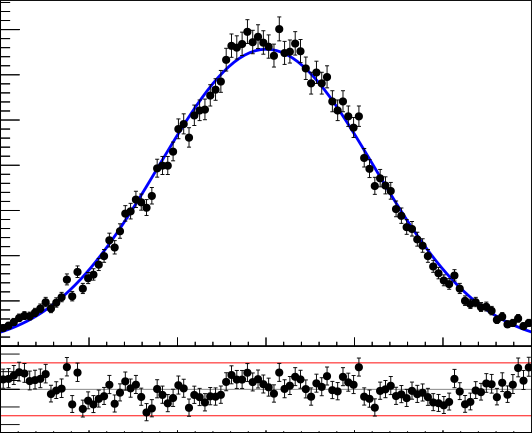
\includegraphics[width=0.9\textwidth]{BsDsK_TD/Time_Resolution/Fit_Pull_DsK_MC_LTUB}};
            \begin{scope}[x={(image.south east)},y={(image.north west)}]
                \foreach \x in {0, ..., 6}
                {
                    \tikzmath{\xpos = (\x / 6); \xtext = \x - 3;}
                    \node at (\xpos, -0.025) {\(\pgfmathprintnumber[fixed,precision=0,fixed zerofill=true]{\xtext}\)};
                }
                \node[anchor=east] at (0.005, .215) {\(0\)};
                \foreach \y in {1, ..., 7}
                {
                    \tikzmath{\ypos = (\y / 7) * 0.729 + .203; \ytext = 100 * \y;}
                    \node[anchor=east] at (0.005, \ypos) {\(\pgfmathprintnumber[fixed,precision=0,fixed zerofill=true,1000 sep={}]{\ytext}\)};
                }
                \foreach \p in {0, ..., 4}
                {
                    \tikzmath{\ypos = (\p / 4) * 0.163 + .02; \ptext = (\p - 2) * 2;}
                    \node[anchor=east] at (0.005, \ypos) {\(\scriptstyle\pgfmathprintnumber[fixed,precision=0,fixed zerofill=true]{\ptext}\)};
                }
                \node[anchor=east] at (1.0, -0.08) {\({t/\dt}\)};
                \node[rotate=90,anchor=east,inner xsep=0pt,outer xsep=0pt] at (-0.12, 1.0) {\({\text{Candidates}/0.06}\)};
                \node[anchor=west] at (0.06, 0.92) {\Large\lhcb};
            \end{scope}
        \end{tikzpicture}
        \caption{Simulated \BsDsK~events.}
    \end{subfigure}
    \par\bigskip
    \begin{subfigure}{.8\textwidth} \centerfloat
        \begin{tikzpicture}
            \node[anchor=south west,inner sep=0] (image) at (0,0) {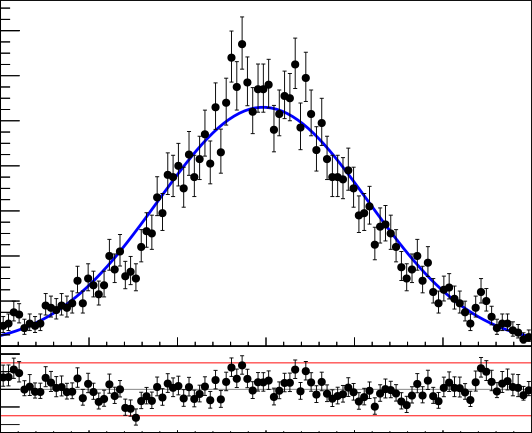
\includegraphics[width=0.9\textwidth]{BsDsK_TD/Time_Resolution/Fit_Pull_Ds_MC}};
            \begin{scope}[x={(image.south east)},y={(image.north west)}]
                \foreach \x in {0, ..., 6}
                {
                    \tikzmath{\xpos = (\x / 6); \xtext = \x - 3;}
                    \node at (\xpos, -0.025) {\(\pgfmathprintnumber[fixed,precision=0,fixed zerofill=true]{\xtext}\)};
                }
                \node[anchor=east] at (0.005, .215) {\(0\)};
                \foreach \y in {1, ..., 7}
                {
                    \tikzmath{\ypos = (\y / 7) * 0.726 + .203; \ytext = 20 * \y;}
                    \node[anchor=east] at (0.005, \ypos) {\(\pgfmathprintnumber[fixed,precision=0,fixed zerofill=true,1000 sep={}]{\ytext}\)};
                }
                \foreach \p in {0, ..., 4}
                {
                    \tikzmath{\ypos = (\p / 4) * 0.163 + .02; \ptext = (\p - 2) * 2;}
                    \node[anchor=east] at (0.005, \ypos) {\(\scriptstyle\pgfmathprintnumber[fixed,precision=0,fixed zerofill=true]{\ptext}\)};
                }
                \node[anchor=east] at (1.0, -0.08) {\({t/\dt}\)};
                \node[rotate=90,anchor=east,inner xsep=0pt,outer xsep=0pt] at (-0.12, 1.0) {\({\text{Candidates}/0.06}\)};
                \node[anchor=west] at (0.06, 0.92) {\Large\lhcb};
            \end{scope}
        \end{tikzpicture}
        \caption{Simulated prompt~\Dspm~events.}
    \end{subfigure}
    \caption{
        Gaussian fits to the \(t/\dt\)~distributions of simulated~\BsDsK events and simulated prompt~\Dspm events.}
    \label{fig:BsDsK_TD_Res_MC}
\end{figure}

Possible differences between these samples is further investigated by inspecting the dependence of the decay-time resolution on the kinematic variable in which prompt~\Dspm and signal \Bs~decays differ the most.
This variable is the companion track~\pt, and to determine this dependence the prompt~\Dspm sample is binned in this variable, after which the same procedure is used to determine the decay-time resolution in each of those bins.
The result of this binned analysis is shown in \cref{fig:BsDsK_TD_Res_PtBins,tab:BsDsK_TD_Res_PtBins}, the latter of which also contains the used binning scheme.
The results show no significant \pt~dependence, except for the highest bin, where low statistics interfere with the determination of~\(s_{0}\) and~\(s_{1}\). 
%
\begin{table}[hb] \centerfloat
    \caption{
        Decay-time resolution corrections of the prompt~\Dspm data sample, in bins of the companion track~\pt.}
    \label{tab:BsDsK_TD_Res_PtBins}
    \rowcolors{2}{tableshade}{}
    \begin{tabular}{cS[table-format=2.1(1)]S[table-format=1.3(3)]}
        \toprule
        \(\pt\)~(\si{\MeVc}) & {\(s_{0}\)~(\si{\fs})} & {\(s_{1}\)} \tabularnewline
        \midrule
        \(\0500\,-\,\0850\) & 59.7 +- 0.4 & 1.239 +- 0.045 \tabularnewline
        \(\0850\,-\, 1150\) & 60.8 +- 0.4 & 1.292 +- 0.047 \tabularnewline
        \( 1150\,-\, 1600\) & 60.3 +- 0.4 & 1.247 +- 0.047 \tabularnewline
        \( 1600\,-\, 2500\) & 63.8 +- 0.5 & 1.388 +- 0.059 \tabularnewline
        \aligncell{r}{\(> \num{2500}\)} & 74.7 +- 1.0 & 2.222 +- 0.106 \tabularnewline
        \bottomrule
    \end{tabular}
\end{table}
%
\begin{figure}[p] \centerfloat
    \fontsize{7}{8.4}\selectfont
    \begin{subfigure}{.48\textwidth} \centerfloat
        \begin{tikzpicture}
            \node[anchor=south west,inner sep=0] (image) at (0,0) {\includegraphics[width=0.9\textwidth]{BsDsK_TD/Time_Resolution/CombinationLinear_ALL_PtBin00_eff_sigma}};
            \begin{scope}[x={(image.south east)},y={(image.north west)}]
                \foreach \x in {0, ..., 10}
                {
                    \tikzmath{\xpos = (\x / 10); \xtext = 10 * \x;}
                    \node at (\xpos, -0.033) {\(\pgfmathprintnumber[fixed,precision=0,fixed zerofill=true]{\xtext}\)};
                }
                \foreach \y in {0, ..., 10}
                {
                    \tikzmath{\ypos = (\y / 10); \ytext = 10 * \y;}
                    \node[anchor=east] at (0.005, \ypos) {\(\pgfmathprintnumber[fixed,precision=0,fixed zerofill=true]{\ytext}\)};
                }
                % Legend
                {
                    \fontsize{6}{7.2}\selectfont
                    \node[anchor=base west] at (0.14, 0.843) {Prompt~\Dspm data};
                    \node[anchor=base west] at (0.14, 0.768) {\BsDsK};
                    \node[anchor=base west] at (0.14, 0.708) {data};
                }
                \node[anchor=east] at (1.0, -0.10) {Per-event decay-time error~\dt~\([\si{\fs}]\)};
                \node[rotate=90,anchor=east,inner xsep=0pt,outer xsep=0pt] at (-0.12, 1.0) {Decay-time resolution~\({\sigma~[\si{\fs}]}\)};
                \node[anchor=west] at (0.055, 0.94) {\fontsize{10}{12}\selectfont \lhcb};
            \end{scope}
        \end{tikzpicture}
        \caption{\(500<\pt/(\si{\MeVc})< 850\)\rlap{.}}
    \end{subfigure} \hfill%
    \begin{subfigure}{.48\textwidth} \centerfloat
        \begin{tikzpicture}
            \node[anchor=south west,inner sep=0] (image) at (0,0) {\includegraphics[width=0.9\textwidth]{BsDsK_TD/Time_Resolution/CombinationLinear_ALL_PtBin01_eff_sigma}};
            \begin{scope}[x={(image.south east)},y={(image.north west)}]
                \foreach \x in {0, ..., 10}
                {
                    \tikzmath{\xpos = (\x / 10); \xtext = 10 * \x;}
                    \node at (\xpos, -0.033) {\(\pgfmathprintnumber[fixed,precision=0,fixed zerofill=true]{\xtext}\)};
                }
                \foreach \y in {0, ..., 10}
                {
                    \tikzmath{\ypos = (\y / 10); \ytext = 10 * \y;}
                    \node[anchor=east] at (0.005, \ypos) {\(\pgfmathprintnumber[fixed,precision=0,fixed zerofill=true]{\ytext}\)};
                }
                % Legend
                {
                    \fontsize{6}{7.2}\selectfont
                    \node[anchor=base west] at (0.14, 0.843) {Prompt~\Dspm data};
                    \node[anchor=base west] at (0.14, 0.768) {\BsDsK};
                    \node[anchor=base west] at (0.14, 0.708) {data};
                }
                \node[anchor=east] at (1.0, -0.10) {Per-event decay-time error~\dt~\([\si{\fs}]\)};
                \node[rotate=90,anchor=east,inner xsep=0pt,outer xsep=0pt] at (-0.12, 1.0) {Decay-time resolution~\({\sigma~[\si{\fs}]}\)};
                \node[anchor=west] at (0.055, 0.94) {\fontsize{10}{12}\selectfont \lhcb};
            \end{scope}
        \end{tikzpicture}
        \caption{\(850<\pt/(\si{\MeVc})<1150\)\rlap{.}}
    \end{subfigure}
    \par\bigskip
    \begin{subfigure}{.48\textwidth} \centerfloat
        \begin{tikzpicture}
            \node[anchor=south west,inner sep=0] (image) at (0,0) {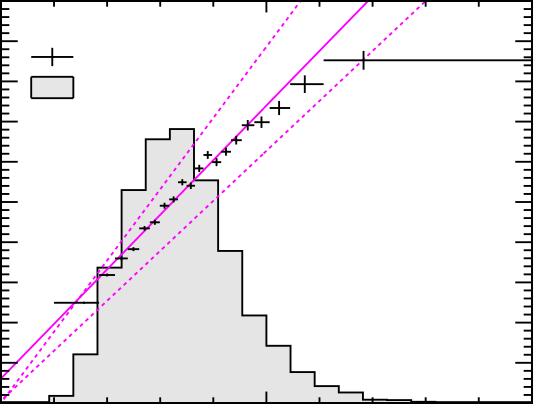
\includegraphics[width=0.9\textwidth]{BsDsK_TD/Time_Resolution/CombinationLinear_ALL_PtBin02_eff_sigma}};
            \begin{scope}[x={(image.south east)},y={(image.north west)}]
                \foreach \x in {0, ..., 10}
                {
                    \tikzmath{\xpos = (\x / 10); \xtext = 10 * \x;}
                    \node at (\xpos, -0.033) {\(\pgfmathprintnumber[fixed,precision=0,fixed zerofill=true]{\xtext}\)};
                }
                \foreach \y in {0, ..., 10}
                {
                    \tikzmath{\ypos = (\y / 10); \ytext = 10 * \y;}
                    \node[anchor=east] at (0.005, \ypos) {\(\pgfmathprintnumber[fixed,precision=0,fixed zerofill=true]{\ytext}\)};
                }
                % Legend
                {
                    \fontsize{6}{7.2}\selectfont
                    \node[anchor=base west] at (0.14, 0.843) {Prompt~\Dspm data};
                    \node[anchor=base west] at (0.14, 0.768) {\BsDsK};
                    \node[anchor=base west] at (0.14, 0.708) {data};
                }
                \node[anchor=east] at (1.0, -0.10) {Per-event decay-time error~\dt~\([\si{\fs}]\)};
                \node[rotate=90,anchor=east,inner xsep=0pt,outer xsep=0pt] at (-0.12, 1.0) {Decay-time resolution~\({\sigma~[\si{\fs}]}\)};
                \node[anchor=west] at (0.055, 0.94) {\fontsize{10}{12}\selectfont \lhcb};
            \end{scope}
        \end{tikzpicture}
        \caption{\(1150<\pt/(\si{\MeVc})<1600\)\rlap{.}}
    \end{subfigure}
    \par\bigskip
    \begin{subfigure}{.48\textwidth} \centerfloat
        \begin{tikzpicture}
            \node[anchor=south west,inner sep=0] (image) at (0,0) {\includegraphics[width=0.9\textwidth]{BsDsK_TD/Time_Resolution/CombinationLinear_ALL_PtBin03_eff_sigma}};
            \begin{scope}[x={(image.south east)},y={(image.north west)}]
                \foreach \x in {0, ..., 10}
                {
                    \tikzmath{\xpos = (\x / 10); \xtext = 10 * \x;}
                    \node at (\xpos, -0.033) {\(\pgfmathprintnumber[fixed,precision=0,fixed zerofill=true]{\xtext}\)};
                }
                \foreach \y in {0, ..., 10}
                {
                    \tikzmath{\ypos = (\y / 10); \ytext = 10 * \y;}
                    \node[anchor=east] at (0.005, \ypos) {\(\pgfmathprintnumber[fixed,precision=0,fixed zerofill=true]{\ytext}\)};
                }
                % Legend
                {
                    \fontsize{6}{7.2}\selectfont
                    \node[anchor=base west] at (0.14, 0.843) {Prompt~\Dspm data};
                    \node[anchor=base west] at (0.14, 0.768) {\BsDsK};
                    \node[anchor=base west] at (0.14, 0.708) {data};
                }
                \node[anchor=east] at (1.0, -0.10) {Per-event decay-time error~\dt~\([\si{\fs}]\)};
                \node[rotate=90,anchor=east,inner xsep=0pt,outer xsep=0pt] at (-0.12, 1.0) {Decay-time resolution~\({\sigma~[\si{\fs}]}\)};
                \node[anchor=west] at (0.055, 0.94) {\fontsize{10}{12}\selectfont \lhcb};
            \end{scope}
        \end{tikzpicture}
        \caption{\(1600<\pt/(\si{\MeVc})<2500\)\rlap{.}}
    \end{subfigure} \hfill%
    \begin{subfigure}{.48\textwidth} \centerfloat
        \begin{tikzpicture}
            \node[anchor=south west,inner sep=0] (image) at (0,0) {\includegraphics[width=0.9\textwidth]{BsDsK_TD/Time_Resolution/CombinationLinear_ALL_PtBin04_eff_sigma}};
            \begin{scope}[x={(image.south east)},y={(image.north west)}]
                \foreach \x in {0, ..., 10}
                {
                    \tikzmath{\xpos = (\x / 10); \xtext = 10 * \x;}
                    \node at (\xpos, -0.033) {\(\pgfmathprintnumber[fixed,precision=0,fixed zerofill=true]{\xtext}\)};
                }
                \foreach \y in {0, ..., 10}
                {
                    \tikzmath{\ypos = (\y / 10); \ytext = 10 * \y;}
                    \node[anchor=east] at (0.005, \ypos) {\(\pgfmathprintnumber[fixed,precision=0,fixed zerofill=true]{\ytext}\)};
                }
                \node[anchor=east] at (1.0, -0.10) {Per-event decay-time error~\dt~\([\si{\fs}]\)};
                \node[rotate=90,anchor=east,inner xsep=0pt,outer xsep=0pt] at (-0.12, 1.0) {Decay-time resolution~\({\sigma~[\si{\fs}]}\)};
                \node[anchor=west] at (0.055, 0.94) {\fontsize{10}{12}\selectfont \lhcb};
            \end{scope}
        \end{tikzpicture}
        \caption{\(\pt>\SI{2500}{\MeVc}\)\rlap{.}}
    \end{subfigure}
    \caption{
        Measured resolution of the prompt~\Dspm data sample, split in five bins of companion track~\pt.}
    \label{fig:BsDsK_TD_Res_PtBins}
\end{figure}

\clearpage

The final validation checks the dependence of the resolution on the \Bs~decay time.
Since the prompt \Dspm~sample only consists of candidates with true decay time zero, it is unsuitable to verify this dependence.
Rather, it is performed on the sample of simulated \BsDsK~events introduced above.
The results are shown in \cref{fig:BsDsK_TD_Res_tBins,tab:BsDsK_TD_Res_tBins}.
All values are compatible with the result in \cref{tab:BsDsK_TD_Res_MC}, and the resolution is found not to depend on the \Bs~decay time.
%
\begin{table}[hb] \centerfloat
    \caption{
        Results of the decay-time resolution determinations on simulated \BsDsK~events in bins of the \Bs~candidate decay time, using both a linear fit with the constant term fixed to zero.}
    \label{tab:BsDsK_TD_Res_tBins}
    \rowcolors{2}{tableshade}{}
    \begin{tabular}{cS[table-format=1.3(3)]S[table-format=2.1(1)]S[table-format=1.3(3)]}
        \toprule
        \(t~(\si{\ps})\)     & {\(s_{1}\)}    & \tabularnewline
        \midrule
        \(0\z\0\,-\,\00.5\)  & 1.178 +- 0.032 & \tabularnewline
        \(  0.5\,-\,\00.8\)  & 1.185 +- 0.021 & \tabularnewline
        \(  0.8\,-\,\01.5\)  & 1.204 +- 0.024 & \tabularnewline
        \(  1.5\,-\,\02.5\)  & 1.196 +- 0.026 & \tabularnewline
        \(  2.5\,-\,10\z\0\) & 1.189 +- 0.020 & \tabularnewline
        \bottomrule
    \end{tabular}
\end{table}
%
\begin{figure}[p] \centerfloat
    \fontsize{7}{8.4}\selectfont
    \begin{subfigure}{.48\textwidth} \centerfloat
        \begin{tikzpicture}
            \node[anchor=south west,inner sep=0] (image) at (0,0) {\includegraphics[width=0.9\textwidth]{BsDsK_TD/Time_Resolution/CombinationLinear_DsK_MC_LTUB_TrecBin00_eff_sigma}};
            \begin{scope}[x={(image.south east)},y={(image.north west)}]
                \foreach \x in {0, ..., 10}
                {
                    \tikzmath{\xpos = (\x / 10); \xtext = 10 * \x;}
                    \node at (\xpos, -0.033) {\(\pgfmathprintnumber[fixed,precision=0,fixed zerofill=true]{\xtext}\)};
                }
                \foreach \y in {0, ..., 10}
                {
                    \tikzmath{\ypos = (\y / 10); \ytext = 10 * \y;}
                    \node[anchor=east] at (0.005, \ypos) {\(\pgfmathprintnumber[fixed,precision=0,fixed zerofill=true]{\ytext}\)};
                }
                % Legend
                {
                    \fontsize{6}{7.2}\selectfont
                    \node[anchor=base west] at (0.14, 0.843) {Simulated~data};
                    \node[anchor=base west] at (0.14, 0.768) {\BsDsK};
                    \node[anchor=base west] at (0.14, 0.708) {data};
                }
                \node[anchor=east] at (1.0, -0.10) {Per-event decay-time error~\dt~\([\si{\fs}]\)};
                \node[rotate=90,anchor=east,inner xsep=0pt,outer xsep=0pt] at (-0.12, 1.0) {Decay-time resolution~\({\sigma~[\si{\fs}]}\)};
                \node[anchor=west] at (0.055, 0.94) {\fontsize{10}{12}\selectfont \lhcb};
            \end{scope}
        \end{tikzpicture}
        \caption{\(0<t/\si{\ps}<0.5\)\rlap{.}}
    \end{subfigure} \hfill%
    \begin{subfigure}{.48\textwidth} \centerfloat
        \begin{tikzpicture}
            \node[anchor=south west,inner sep=0] (image) at (0,0) {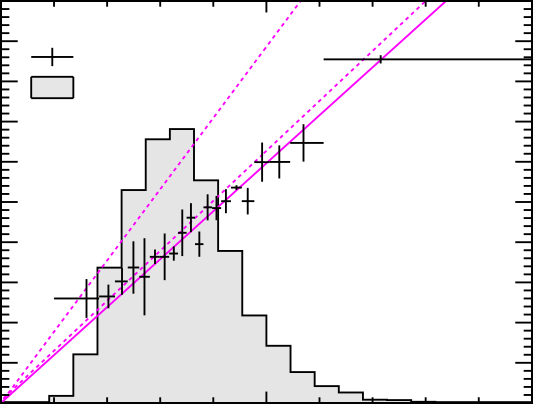
\includegraphics[width=0.9\textwidth]{BsDsK_TD/Time_Resolution/CombinationLinear_DsK_MC_LTUB_TrecBin01_eff_sigma}};
            \begin{scope}[x={(image.south east)},y={(image.north west)}]
                \foreach \x in {0, ..., 10}
                {
                    \tikzmath{\xpos = (\x / 10); \xtext = 10 * \x;}
                    \node at (\xpos, -0.033) {\(\pgfmathprintnumber[fixed,precision=0,fixed zerofill=true]{\xtext}\)};
                }
                \foreach \y in {0, ..., 10}
                {
                    \tikzmath{\ypos = (\y / 10); \ytext = 10 * \y;}
                    \node[anchor=east] at (0.005, \ypos) {\(\pgfmathprintnumber[fixed,precision=0,fixed zerofill=true]{\ytext}\)};
                }
                % Legend
                {
                    \fontsize{6}{7.2}\selectfont
                    \node[anchor=base west] at (0.14, 0.843) {Simulated~data};
                    \node[anchor=base west] at (0.14, 0.768) {\BsDsK};
                    \node[anchor=base west] at (0.14, 0.708) {data};
                }
                \node[anchor=east] at (1.0, -0.10) {Per-event decay-time error~\dt~\([\si{\fs}]\)};
                \node[rotate=90,anchor=east,inner xsep=0pt,outer xsep=0pt] at (-0.12, 1.0) {Decay-time resolution~\({\sigma~[\si{\fs}]}\)};
                \node[anchor=west] at (0.055, 0.94) {\fontsize{10}{12}\selectfont \lhcb};
            \end{scope}
        \end{tikzpicture}
        \caption{\(0.5<t/\si{\ps}<0.8\)\rlap{.}}
    \end{subfigure}
    \par\bigskip
    \begin{subfigure}{.48\textwidth} \centerfloat
        \begin{tikzpicture}
            \node[anchor=south west,inner sep=0] (image) at (0,0) {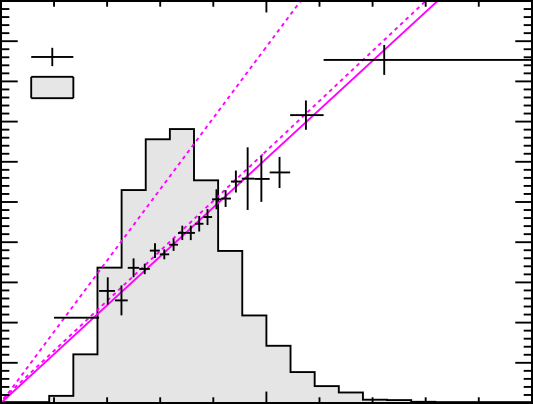
\includegraphics[width=0.9\textwidth]{BsDsK_TD/Time_Resolution/CombinationLinear_DsK_MC_LTUB_TrecBin02_eff_sigma}};
            \begin{scope}[x={(image.south east)},y={(image.north west)}]
                \foreach \x in {0, ..., 10}
                {
                    \tikzmath{\xpos = (\x / 10); \xtext = 10 * \x;}
                    \node at (\xpos, -0.033) {\(\pgfmathprintnumber[fixed,precision=0,fixed zerofill=true]{\xtext}\)};
                }
                \foreach \y in {0, ..., 10}
                {
                    \tikzmath{\ypos = (\y / 10); \ytext = 10 * \y;}
                    \node[anchor=east] at (0.005, \ypos) {\(\pgfmathprintnumber[fixed,precision=0,fixed zerofill=true]{\ytext}\)};
                }
                % Legend
                {
                    \fontsize{6}{7.2}\selectfont
                    \node[anchor=base west] at (0.14, 0.843) {Simulated~data};
                    \node[anchor=base west] at (0.14, 0.768) {\BsDsK};
                    \node[anchor=base west] at (0.14, 0.708) {data};
                }
                \node[anchor=east] at (1.0, -0.10) {Per-event decay-time error~\dt~\([\si{\fs}]\)};
                \node[rotate=90,anchor=east,inner xsep=0pt,outer xsep=0pt] at (-0.12, 1.0) {Decay-time resolution~\({\sigma~[\si{\fs}]}\)};
                \node[anchor=west] at (0.055, 0.94) {\fontsize{10}{12}\selectfont \lhcb};
            \end{scope}
        \end{tikzpicture}
        \caption{\(0.8<t/\si{\ps}<1.5\)\rlap{.}}
    \end{subfigure}
    \par\bigskip
    \begin{subfigure}{.48\textwidth} \centerfloat
        \begin{tikzpicture}
            \node[anchor=south west,inner sep=0] (image) at (0,0) {\includegraphics[width=0.9\textwidth]{BsDsK_TD/Time_Resolution/CombinationLinear_DsK_MC_LTUB_TrecBin03_eff_sigma}};
            \begin{scope}[x={(image.south east)},y={(image.north west)}]
                \foreach \x in {0, ..., 10}
                {
                    \tikzmath{\xpos = (\x / 10); \xtext = 10 * \x;}
                    \node at (\xpos, -0.033) {\(\pgfmathprintnumber[fixed,precision=0,fixed zerofill=true]{\xtext}\)};
                }
                \foreach \y in {0, ..., 10}
                {
                    \tikzmath{\ypos = (\y / 10); \ytext = 10 * \y;}
                    \node[anchor=east] at (0.005, \ypos) {\(\pgfmathprintnumber[fixed,precision=0,fixed zerofill=true]{\ytext}\)};
                }
                % Legend
                {
                    \fontsize{6}{7.2}\selectfont
                    \node[anchor=base west] at (0.14, 0.843) {Simulated~data};
                    \node[anchor=base west] at (0.14, 0.768) {\BsDsK};
                    \node[anchor=base west] at (0.14, 0.708) {data};
                }
                \node[anchor=east] at (1.0, -0.10) {Per-event decay-time error~\dt~\([\si{\fs}]\)};
                \node[rotate=90,anchor=east,inner xsep=0pt,outer xsep=0pt] at (-0.12, 1.0) {Decay-time resolution~\({\sigma~[\si{\fs}]}\)};
                \node[anchor=west] at (0.055, 0.94) {\fontsize{10}{12}\selectfont \lhcb};
            \end{scope}
        \end{tikzpicture}
        \caption{\(1.5<t/\si{\ps}<2.5\)\rlap{.}}
    \end{subfigure} \hfill%
    \begin{subfigure}{.48\textwidth} \centerfloat
        \begin{tikzpicture}
            \node[anchor=south west,inner sep=0] (image) at (0,0) {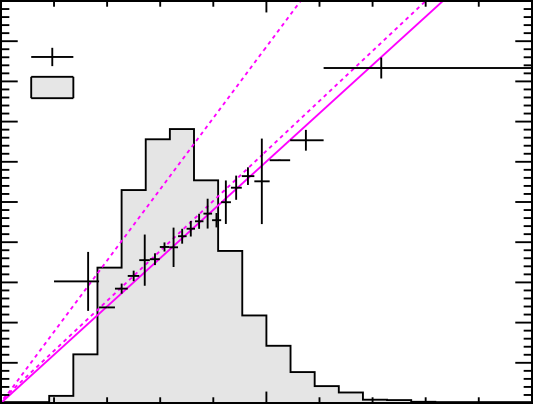
\includegraphics[width=0.9\textwidth]{BsDsK_TD/Time_Resolution/CombinationLinear_DsK_MC_LTUB_TrecBin04_eff_sigma}};
            \begin{scope}[x={(image.south east)},y={(image.north west)}]
                \foreach \x in {0, ..., 10}
                {
                    \tikzmath{\xpos = (\x / 10); \xtext = 10 * \x;}
                    \node at (\xpos, -0.033) {\(\pgfmathprintnumber[fixed,precision=0,fixed zerofill=true]{\xtext}\)};
                }
                \foreach \y in {0, ..., 10}
                {
                    \tikzmath{\ypos = (\y / 10); \ytext = 10 * \y;}
                    \node[anchor=east] at (0.005, \ypos) {\(\pgfmathprintnumber[fixed,precision=0,fixed zerofill=true]{\ytext}\)};
                }
                % Legend
                {
                    \fontsize{6}{7.2}\selectfont
                    \node[anchor=base west] at (0.14, 0.843) {Simulated~data};
                    \node[anchor=base west] at (0.14, 0.768) {\BsDsK};
                    \node[anchor=base west] at (0.14, 0.708) {data};
                }
                \node[anchor=east] at (1.0, -0.10) {Per-event decay-time error~\dt~\([\si{\fs}]\)};
                \node[rotate=90,anchor=east,inner xsep=0pt,outer xsep=0pt] at (-0.12, 1.0) {Decay-time resolution~\({\sigma~[\si{\fs}]}\)};
                \node[anchor=west] at (0.055, 0.94) {\fontsize{10}{12}\selectfont \lhcb};
            \end{scope}
        \end{tikzpicture}
        \caption{\(2.5<t/\si{\ps}<10 \)\rlap{.}}
    \end{subfigure}
    \caption{
        Measured resolution on simulated \BsDsK~events, split in five bins of \Bs~candidate decay time.}
    \label{fig:BsDsK_TD_Res_tBins}
\end{figure}

\clearpage
\subsection{Systematic effects} \label{sec:BsDsK_TD_Res_Syst}

In the resolution calibration procedure, a double Gaussian~PDF is necessary to obtain a good fit of the decay times.
In order to validate this method, two alternative approaches on the prompt~\Ds data sample are considered, that reduce the contribution of events in the tail of the distribution:
%
\begin{enumerate}
    \item Using only the width of the narrow Gaussian, instead of \cref{eqn:BsDsK_TD_Res_EffectiveSigma}.
        The wider one is still used in the fits, but only the narrow Gaussian is assumed to be representative of the actual decay-time resolution.
    \item Fitting a single Gaussian over a wider decay-time window:~\({[-3.25, 1.3]\dt}\), where \dt~is the centre of the respective per-event decay-time error bin.
        This approach narrows the lower decay-time tail and slightly extends it on the other side, in order to reduce the effect of the tail.
\end{enumerate}
%
The resulting calibration equations are as follows,
%
\begin{subequations} \label{eqn:BsDsK_TD_Res_Syst}
    \begin{align}
        \sigma = (\num{1.243 +- 0.044}) \dt \rlap{,} \label{eqn:BsDsK_TD_Res_Syst1} \\
        \sigma = (\num{1.772 +- 0.012}) \dt \rlap{,} \label{eqn:BsDsK_TD_Res_Syst2}
    \end{align}
\end{subequations}
%
respectively, where again the constant term is found to be negligible, and hence fixed to zero.
These equations are used to evaluate systematic effects on the decay-time resolution model.
They are also shown in \cref{fig:BsDsK_TD_Res_Nominal}.

\clearpage
\section{Flavour tagging} \label{sec:BsDsK_TD_Tagging}
It is necessary to know the initial flavour of the observed signal \Bs~mesons,~\ie, whether it was produced as a \Bs~or a \Bsb~meson.
The \BsorBsb~meson hadronises from one of the quarks of a \({\bquark\bquarkbar}\)~pair produced in the \({\proton\proton}\)~collision.
The quark on the opposite side~(OS, see \cref{fig:BsDsK_TD_Tagging_Schematic}) of the signal pair similarly hadronises into a \bquark~hadron, which also decays.
By reconstructing this decay, the flavour of that hadron can be determined.
The decays reconstructed this way are semileptonic \bquark-meson decays and charmed \bquark-hadron decays.
Such decays must be self-tagging, meaning the flavour at decay must be inferable directly from the decay products.
These include~\BdDmunu and~\BpJpsiK.
However, even with self-tagging decays, neutral \bquark~mesons can still oscillate before decaying, resulting in wrong tags.
For charged \bquark~hadrons, no oscillation occurs, and it is additionally possible to infer the flavour from the total decay vertex charge.
%
\begin{figure}[hp] \centerfloat
    \begin{tikzpicture}
        \draw [lightgray,fill=lightgray] (4, 1.5) circle (2.5 and 5.5); % PV blob
        \node [lightgray,anchor=south] at (4, 7) {PV};
        \draw [thick,->] (0, 0) -- (2.9, 0) node [at start,anchor=north west] {\normalsize \proton}; % proton 1
        \draw [thick,->] (6, 0) -- (3.1, 0) node [at start,anchor=north east] {\normalsize \proton}; % proton 2
        \draw [dashed] (\linewidth, 0) -- (6, 0); % dashed horizontal line
        \node [anchor=south east] at (\linewidth, 0) {same side};
        \node [anchor=north east] at (\linewidth, 0) {opposite side};
        \draw [supporta,fill=supporta] (3, 0) circle (0.1); % PV dot

        % SS
        \draw [supportd,fill=supportd,rotate around={30:(4,2)}] (4, 2) circle (1.3 and 0.8); % Bs SS blob
        \draw [lightgray,fill=lightgray] (8.5, 3.5) circle (1 and 2); % SS SV blob
        \node [lightgray,anchor=south] at (8.5, 5.5) {SV};
        \draw [supportd,very thick,->] (4, 2) -- (7.5, 3.5) node [above,sloped,pos=0.70] {signal~\Bs}; % Bs SS decay arrow
        \draw [supportb,fill=supportb,rotate around={-30:(4,5)}] (4, 5) circle (1.3 and 0.8); % K+ SS blob
        \draw [very thick,supporta] (3, 0) -- (3.575, 1.726); % line to Bs SS
        \draw [supporta,fill=supporta] (3.575, 1.726) circle (0.45) node [black] {\bquarkbar}; % SS bbar quark
        \draw [very thick,supportc] (4.475, 2.274) -- (3, 3.45); % SS s quark line 1
        \draw [supportc,fill=supportc] (4.475, 2.274) circle (0.45) node [black] {\squark}; % SS s quark
        \draw [supportc,fill=supportc] (3, 3.45) circle (0.1); % SS s quarks origin
        \draw [very thick,supportc] (4.475, 4.726) -- (3, 3.45); % SS s quark line 2
        \draw [supportb,very thick,->] (4, 5) -- (6, 6.5); % SS K+ decay arrow
        \draw [supportc,fill=supportc] (6.331, 6.875) circle (0.5) node [black] {\Kp}; % K+ SS decay particle
        \node [anchor=west] at (7, 6.875) {SS~kaon};
        \draw [supportc,fill=supportc] (4.475, 4.726) circle (0.45) node [black] {\squarkbar}; % SS sbar quark
        \draw [supportc,fill=supportc] (3.575, 5.274) circle (0.45) node [black] {\uquark}; % SS u quark

        \draw [supportc,fill=supportc] (8.5, 4.25) circle (0.5) node [black] {\Dspm}; % Ds+- SS decay particle
        \draw [supportc,fill=supportc] (8.5, 2.75) circle (0.5) node [black] {\Kmp}; % K-+ SS decay particle

        % OS
        \draw [supportd,fill=supportd,rotate around={-30:(4,-2)}] (4, -2) circle (1.3 and 0.8); % BX OS blob
        \draw [lightgray,fill=lightgray] (9.5, -2) circle (2 and 1); % OS SV blob
        \node [lightgray,anchor=south] at (9.5, -1) {SV};
        \node [align=left] at (9.5, -2) {\decay{\bquark}{\cquark}\\ \decay{\bquark}{\PX\ellm\neub}};
        \node [anchor=west,align=left] at (11.5, -2) {OS~charm\\OS~lepton};
        \node [anchor=north] at (9.5, -3) {OS vertex charge};
        \draw [supportd,very thick,->] (4, -2) -- (7.5, -2); % BX OS decay arrow
        \draw [very thick,supporta] (3, 0) -- (3.575, -1.726); % line to BX OS
        \draw [supporta,fill=supporta] (3.575, -1.726) circle (0.45) node [black] {\bquark}; % OS b quark
        \draw [supportc,fill=supportc] (4.475, -2.274) circle (0.45) node [black] {\(\overline{\quark}\)}; % OS xbar quark
    \end{tikzpicture}
    \caption{
        Schematic overview of the various ways \bquark~mesons are flavour-tagged.
        The top half of the figure represents the part on the same side~(SS) as the signal \Bs~meson, including the SS~kaon tagger.
        The bottom half contains the \bquark~quark on the opposite side~(OS), with the OS~taggers.}
    \label{fig:BsDsK_TD_Tagging_Schematic}
\end{figure}

In addition to OS~tagging, it is also possible to use the \squark~quark from which the signal \Bs~meson hadronises.
This, too, has an accompanying \squarkbar~quark in the \({\bquark\bquarkbar}\)~fragmentation string, which can be used to identify the \BsorBsb~flavour in case it hadronises into a charged kaon.
This form of tagging uses information on the same side~(SS) of the \Bs~meson and is hence called SS~tagging.
Although SS~tagging can be applied using both pions and kaons, due to the presence of many final-state pions in the underlying event the latter is more pure, and as such mainly applied to tag \Bs~mesons.

Each of these procedures carries an inherent uncertainty on the tag decision, due to wrong track assignments, misidentified particles, as well as the aforementioned oscillations of neutral \bquark~mesons.
These uncertainties are combined into a single per-event mistag probability~\(\eta\), and are determined using neural networks trained on self-tagging decays: simulated \BsDsPi~data for SS~tagging, and \decay{\Bp}{\jpsi\Kp} data for OS~tagging.
The final tagging performance is quantified in terms of tagging efficiency~\({\etag = N_{\text{tag}} / N_{\text{all}}}\) and mistag probability~\({\omega = N_{\text{wrong}} / N_{\text{tag}}}\), where \(N_\text{wrong}\), \(N_\text{tag}\), and \(N_\text{all}\) are the number of wrongly tagged events, tagged events, and all events, respectively.

\subsection{Flavour tagging calibration}

The per-event mistag probability is used in the decay-time fit to improve the fit quality by assigning greater weights to better-tagged events.
The calculated per-event mistag probability is compared to the measured mistag probability.
This calibration is done using \BsDsPi~events obtained from data as described in \cref{sec:BsDsK_TD_MD_Fit}.
The conversion from the estimated mistag probability~\(\eta\) to its calibrated equivalent~\(\omega\) is modelled with a linear function,
%
\begin{equation} \label{eqn:BsDsK_TD_Tagging_Parameters}
    \omega(\eta) = \tagp0 + \tagp1 (\eta - \avgeta) \rlap{,}
\end{equation}
%
where \tagp0~and \tagp1~are free parameters and \avgeta~is the average~\(\eta\) of the sample.
In ideal case where no calibration is necessary, \({\tagp0 = 0}\) and \({\tagp1 = 1}\).
In addition to the calibration, the tagging efficiency~\etag, tagging asymmetries~\Dtagp0, \Dtagp1 and~\Detag (defined as the differences in those parameters between tagged~\Bs and tagged~\Bsb candidates), and effective tagging efficiency~\({\eeff = \etag(1 - 2\omega)^2}\) are determined.
The effective tagging efficiency quantifies the effective reduction in statistical sensitivity of the sample as a result of the imperfect flavour tagging.
%
\begin{table}[htb] \centerfloat
    \caption{
        Flavour tagging calibration results.
        The parameters~\tagp0, \tagp1, and~\avgeta are defined as in \cref{eqn:BsDsK_TD_Tagging_Parameters}, and the others as given in the text.}
    \label{tab:BsDsK_TD_Tagging_Calibration}
    \rowcolors{2}{tableshade}{}
    \begin{tabular}{lS[table-format=1.3(3)]S[table-format=1.3(3)]}
        \toprule
        & \centercell{OS} & \centercell{SS} \tabularnewline
        \midrule
        \tagp0 & 0.374 +- 0.006 & 0.441 +- 0.005 \tabularnewline
        \tagp1 & 1.094 +- 0.063 & 1.084 +- 0.068 \tabularnewline
        \avgeta & \centercell{0.370} & \centercell{0.437} \tabularnewline
        \etag & \SI{37.15 +- 0.17}{\percent} & \SI{63.90 +- 0.17}{\percent} \tabularnewline
        \midrule
        \Dtagp0 & 0.014 +- 0.006 & -0.018 +- 0.004 \tabularnewline
        \Dtagp1 & 0.126 +- 0.062 &  0.130 +- 0.067 \tabularnewline
        \Detag & \SI{-1.14 +- 0.72}{\percent} & \SI{0.82 +- 0.72}{\percent} \tabularnewline
        \hiderowcolors \midrule
        \eeff & \SI{3.89 +- 0.29}{\percent} & \SI{2.08 +- 0.21}{\percent} \tabularnewline
        \bottomrule
    \end{tabular}
\end{table}

The resulting quantities are listed in \cref{tab:BsDsK_TD_Tagging_Calibration}, where OS~refers to the combination of the aforementioned OS~taggers.
The asymmetries in calibration parameters are significantly different from zero, most likely due to differences in production and material interactions between positively and negatively charged particles.
These asymmetries are taken into account in the decay-time fit to extract the \CP-violation parameters.

To use the tagging performance as calibrated on~\BsDsPi, it is necessary to verify the equivalence between decays in that channel and those in~\BsDsK.
This verification is performed on simulated \BsDsPi~and \BsDsK~decays.
As can be seen in \cref{fig:BsDsK_TD_Tagging_MC_Comparison}, the \(\eta\)~distributions of the two samples agree very well in~\(\eta\).
In addition, it is verified that they are similar in the kinematic variables with which the tagging correlates.
The calibration parameters~\tagp0 and~\tagp1 are determined for each sample, both by using the simulation truth information directly as well as the self-tagging decay channel~\BsDsPi (after performing the~\sfit on the \DsmPip~invariant mass).
The results of these calibrations are presented in \cref{tab:BsDsK_TD_Tagging_MC_Calibration}.
The values of \tagp0~and \tagp1~are close to \avgeta~and unity, respectively, which shows that the initial estimate of the mistag probability is close the calibrated one.
%
\begin{table}[htb] \centerfloat
    \caption{
        Flavour tagging calibration results on simulated samples.
        The first two use information on the generated \Bs~mesons, while the last one only uses the self-tagging nature of the decay~\BsDsPi.
        The parameters~\tagp0, \tagp1, and~\avgeta are defined as in \cref{eqn:BsDsK_TD_Tagging_Parameters}.
        The resulting values show compatibility between \BsDsPi~events and \BsDsK~events, as well as between the method using truth information and the one used on actual data.}
    \label{tab:BsDsK_TD_Tagging_MC_Calibration}
    \begin{tabular}{r@{\,}p{.05em}lS[table-format=1.3(3)]S[table-format=1.3(3)]S[table-format=.3]}
        \toprule
        &&    & {\tagp0}       & {\tagp1}       & {\avgeta} \tabularnewline
        \midrule
        \multirow{2}{*}{\BsDsPi} & \multirow{2}{*}{\Big{\{}}
         & OS & 0.361 +- 0.001 & 0.936 +- 0.012 & 0.360 \tabularnewline
        && SS & 0.427 +- 0.001 & 1.186 +- 0.001 & 0.431 \tabularnewline
        \midrule
        \multirow{2}{*}{\BsDsK} & \multirow{2}{*}{\Big{\{}}
         & OS & 0.360 +- 0.001 & 0.936 +- 0.012 & 0.360 \tabularnewline
        && SS & 0.428 +- 0.001 & 1.184 +- 0.010 & 0.431 \tabularnewline
        \midrule
        \multirow{2}{*}{\BsDsPi (\sfit)} & \multirow{2}{*}{\Big{\{}}
         & OS & 0.362 +- 0.002 & 0.931 +- 0.016 & 0.360 \tabularnewline
        && SS & 0.428 +- 0.001 & 1.162 +- 0.015 & 0.431 \tabularnewline
        \bottomrule
    \end{tabular}
\end{table}
%
\begin{figure}[htb] \centerfloat
    \fontsize{7}{8.4}\selectfont
    \begin{subfigure}{.48\textwidth} \centerfloat
        \begin{tikzpicture}
            \node[anchor=south west,inner sep=0] (image) at (0,0) {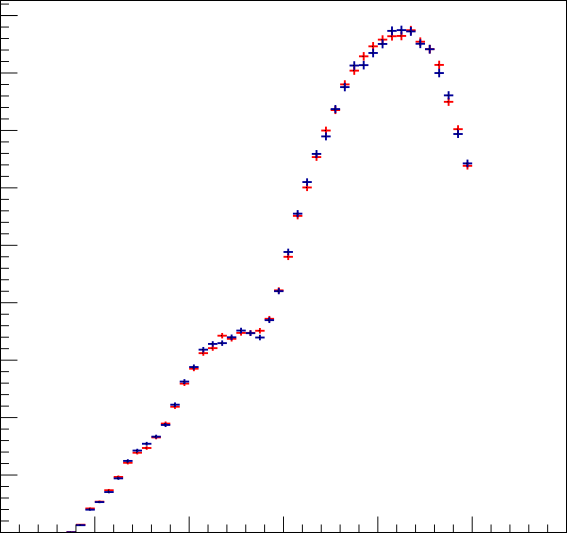
\includegraphics[width=0.9\textwidth]{BsDsK_TD/Tagging/eta_OS_MC}};
            \begin{scope}[x={(image.south east)},y={(image.north west)}]
                \node at (0., -0.025) {\(0\)};
                \foreach \x in {1, ..., 6}
                {
                    \tikzmath{\xpos = (\x / 6); \xtext = 0.1 * \x;}
                    \node at (\xpos, -0.025) {\(\pgfmathprintnumber[fixed,precision=1,fixed zerofill=true]{\xtext}\)};
                }
                \node[anchor=east] at (0.005, 0.) {\(0\)};
                \foreach \y in {1, ..., 9}
                {
                    \tikzmath{\ypos = (\y / 9) * .972; \ytext = 0.005 * \y;}
                    \node[anchor=east] at (0.005, \ypos) {\(\pgfmathprintnumber[fixed,precision=3,fixed zerofill=true]{\ytext}\)};
                }
                \node[anchor=east] at (1.0, -0.09) {\(\eta\)};
                \node[anchor=west] at (0.06, 0.92) {\Large\lhcb};
            \end{scope}
        \end{tikzpicture}
        \caption{OS tagging performance.}
    \end{subfigure} \hfill%
    \begin{subfigure}{.48\textwidth} \centerfloat
        \begin{tikzpicture}
            \node[anchor=south west,inner sep=0] (image) at (0,0) {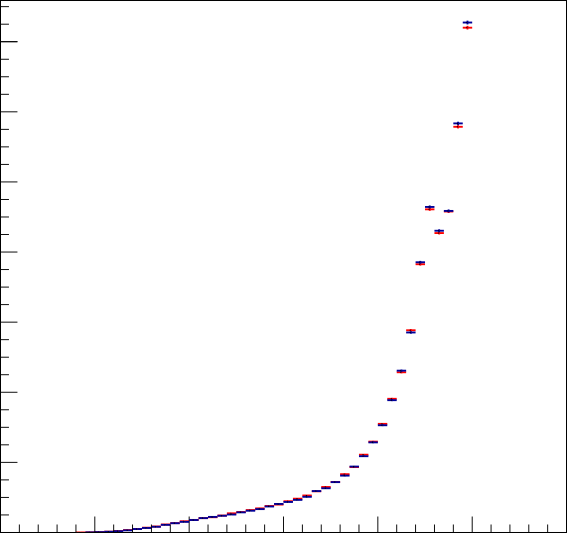
\includegraphics[width=0.9\textwidth]{BsDsK_TD/Tagging/eta_SS_MC}};
            \begin{scope}[x={(image.south east)},y={(image.north west)}]
                \node at (0., -0.025) {\(0\)};
                \foreach \x in {1, ..., 6}
                {
                    \tikzmath{\xpos = (\x / 6); \xtext = 0.1 * \x;}
                    \node at (\xpos, -0.025) {\(\pgfmathprintnumber[fixed,precision=1,fixed zerofill=true]{\xtext}\)};
                }
                \node[anchor=east] at (0.005, 0.) {\(0\)};
                \foreach \y in {1, ..., 7}
                {
                    \tikzmath{\ypos = (\y / 7) * .923; \ytext = 0.02 * \y;}
                    \node[anchor=east] at (0.005, \ypos) {\(\pgfmathprintnumber[fixed,precision=2,fixed zerofill=true]{\ytext}\)};
                }
                \node[anchor=east] at (1.0, -0.09) {\(\eta\)};
                \node[anchor=west] at (0.06, 0.92) {\Large\lhcb};
            \end{scope}
        \end{tikzpicture}
        \caption{SS tagging performance.}
    \end{subfigure}
    \caption{
        Comparison of the tagging performance~\(\eta\) between simulated \BsDsPi~(blue) and \BsDsK~(red) events.}
    \label{fig:BsDsK_TD_Tagging_MC_Comparison}
\end{figure}

\subsection{Combination of taggers}

In order to get one final tagging decision for events with a tagging decision from both the OS~and SS~taggers, the calibrated taggers are combined event-by-event into a single tagging decision, including the mistag probability.
This is done using the tagging combination described in Ref.~\cite{LHCb-PAPER-2011-027}, which takes into account the relative mistag probabilities, and subsequently flipping the tag of each event with mistag probability~\({\omega > 0.5}\).
The resulting (effective) tagging efficiencies are reported in \cref{tab:BsDsK_TD_Tagging_Combination}.
%
\begin{table}[htb] \centerfloat
    \caption{
        Flavour tagging efficiencies after combining the taggers.}
    \label{tab:BsDsK_TD_Tagging_Combination}
    \begin{tabular}{l*{4}{S[table-format=2.2(2)]}}
        \toprule
        \multirow{2}{*}[-2pt]{Tagger} & \multicolumn{2}{c}{\BsDsPi} & \multicolumn{2}{c}{\BsDsK} \tabularnewline
                  \cmidrule(lr){2-3}             \cmidrule(lr){4-5}
                & {\etag~(\%)}  & {\eeff~(\%)} & {\etag~(\%)}  & {\eeff~(\%)} \tabularnewline
        \midrule
        OS~only & 12.94 +- 0.11 & 1.41 +- 0.11 & 13.58 +- 0.44 & 1.44 +- 0.12 \tabularnewline
        \rowcolor{tableshade}
        SS~only & 39.70 +- 0.16 & 1.29 +- 0.13 & 38.65 +- 0.63 & 1.18 +- 0.12 \tabularnewline
        Both    & 24.21 +- 0.14 & 3.10 +- 0.18 & 23.37 +- 0.55 & 3.05 +- 0.20 \tabularnewline
        \midrule
        Total   & 76.85 +- 0.24 & 5.80 +- 0.25 & 75.60 +- 1.30 & 5.67 +- 0.26 \tabularnewline
        \bottomrule
    \end{tabular}
\end{table}

\subsection{Systematic uncertainty}

Several systematic effects give rise to an uncertainty on the tagging parameters.
First of all, the tagging depends on the decay-time resolution and its calibration.
A different proper-time resolution is effectively compensated by a modified tagging calibration.
In order to avoid double counting, and resulting biases in the determination of the \CP-violation parameters, a consistent determination of resolution and tagging is required.
The systematic effect of using a different decay-time resolution model on the tagging is determined for comparison, and found to be negligible.
These results are shown in \cref{tab:BsDsK_TD_Tagging_ResSyst}.
%
\begin{table}[htb] \centerfloat
    \caption{
        Flavour tagging calibration parameters in self-tagging \BsDsPi~events, using the different decay-time resolution models from \cref{eqn:BsDsK_TD_Res_Syst}.
        The nominal results (\cref{tab:BsDsK_TD_Tagging_Calibration}) are also included for comparison.}
    \label{tab:BsDsK_TD_Tagging_ResSyst}
    \begin{tabular}{r@{\,}p{.05em}lS[table-format=.3(3)]S[table-format=1.2(1)]S[table-format=+.3(3)]S[table-format=1.2(1)]}
        \toprule
        \multicolumn{3}{r}{Resolution model} & {\tagp0}       & {\tagp1}     & {\Dtagp0}       & {\Dtagp1} \tabularnewline
        \midrule
        \multirow{3}{*}{OS} & \multirow{3}{*}{\Bigg{\{}}
         & Nominal                           & 0.374 +- 0.006 & 1.09 +- 0.06 &  0.014 +- 0.006 & 0.13 +- 0.06 \tabularnewline
        && \cref{eqn:BsDsK_TD_Res_Syst1}     & 0.393 +- 0.005 & 0.93 +- 0.06 &  0.013 +- 0.006 & 0.13 +- 0.06 \tabularnewline
        && \cref{eqn:BsDsK_TD_Res_Syst2}     & 0.364 +- 0.007 & 1.16 +- 0.07 &  0.014 +- 0.006 & 0.12 +- 0.06 \tabularnewline
        \midrule
        \multirow{3}{*}{SS} & \multirow{3}{*}{\Bigg{\{}}
         & Nominal                           & 0.441 +- 0.005 & 1.08 +- 0.07 & -0.018 +- 0.004 & 0.13 +- 0.07 \tabularnewline
        && \cref{eqn:BsDsK_TD_Res_Syst1}     & 0.450 +- 0.004 & 0.94 +- 0.06 & -0.017 +- 0.004 & 0.13 +- 0.07 \tabularnewline
        && \cref{eqn:BsDsK_TD_Res_Syst2}     & 0.438 +- 0.005 & 1.13 +- 0.07 & -0.018 +- 0.004 & 0.14 +- 0.07 \tabularnewline
        \bottomrule
    \end{tabular}
\end{table}
%
Some variations on the tagging calibration are possible, which reflect the uncertainties on the procedures.
Therefore, the differences with the nominal method are used as systematic uncertainties.
These variations are as follows:
%
\begin{description}
    \item[Calibration method.]
        Rather than calibrating the mistag event-by-event, the events are separated into bins of~\(\eta\), and the calibrated mistag is determined as a constant number for each bin.
    \item[Varying the misidentified background yield.]
        The fraction of background \BsDsK~events used in the multivariate fit to determine the weights of the \BsDsPi~sample is halved and doubled, respectively.
    \item[Varying the combinatorial description.]
        To describe the shape of the combinatorial background in the \DsmPip~mass of the multivariate fit to the \BsDsPi~sample (see \cref{fig:BsDsK_TD_DsPi_MDFit_Results}), the shape of an exponential function plus a constant is used.
        To assess the effect of the choice of combinatorial description, it is fitted with a single exponential and a double exponential, respectively, instead.
\end{description}

The associated systematic uncertainty is defined as the difference in tagging parameters with the nominal method.
The systematic uncertainties from these methods, as well the total systematic uncertainty, are presented in \cref{tab:BsDsK_TD_Tagging_SystOS,tab:BsDsK_TD_Tagging_SystSS}.
The total uncertainties, defined as the sum in quadrature of the systematic and statistical uncertainties, are propagated into the decay-time fit error as described in \cref{sec:BsDsK_TD_TimeFit}.
%
\begin{table}[htb] \centerfloat
    \caption{
        Systematic uncertainties on OS flavour tagging calibration parameters.}
    \label{tab:BsDsK_TD_Tagging_SystOS}
    \sisetup{group-digits=false}
    \begin{tabular}{l*{2}{S[table-format=.4]}S[table-format=.5]S[table-format=.4]}
        \toprule
                                     & {\tagp0} & {\tagp1} & {\Dtagp0} & {\Dtagp1} \tabularnewline
        \midrule
        Calibration method           & 0.0002   & 0.012    & {--}      & {--} \tabularnewline
        \rowcolor{tableshade}
        Misidentified yield          & 0.0001   & 0.0017   & 0.00006   & 0.0009 \tabularnewline
        Combinatorial description    & 0.0004   & 0.0018   & 0.00001   & 0.0015 \tabularnewline
        \midrule
        Total systematic uncertainty & 0.0004   & 0.012    & 0.00006   & 0.0017 \tabularnewline
        \rowcolor{tableshade}
        Statistical uncertainty      & 0.0061   & 0.063    & 0.006     & 0.062 \tabularnewline
        \midrule
        Total uncertainty            & 0.0061   & 0.064    & 0.006     & 0.062 \tabularnewline
        \bottomrule
    \end{tabular}
\end{table}
%
\begin{table}[htb] \centerfloat
    \caption{
        Systematic uncertainties on SS flavour tagging calibration parameters.}
    \label{tab:BsDsK_TD_Tagging_SystSS}
    \sisetup{group-digits=false}
    \begin{tabular}{l*{2}{S[table-format=.4]}S[table-format=.5]S[table-format=.4]}
        \toprule
                                     & {\tagp0} & {\tagp1} & {\Dtagp0} & {\Dtagp1} \tabularnewline
        \midrule
        Calibration method           & 0.0002   & 0.0035   & {--}      & {--} \tabularnewline
        \rowcolor{tableshade}
        Misidentified yield          & 0.0001   & 0.0015   & 0.00009   & 0.0012 \tabularnewline
        Combinatorial description    & 0.0001   & 0.0041   & 0.00015   & 0.0009 \tabularnewline
        \midrule
        Total systematic uncertainty & 0.0002   & 0.006    & 0.00017   & 0.0015 \tabularnewline
        \rowcolor{tableshade}
        Statistical uncertainty      & 0.0047   & 0.068    & 0.004     & 0.067 \tabularnewline
        \midrule
        Total uncertainty            & 0.0047   & 0.068    & 0.004     & 0.067 \tabularnewline
        \bottomrule
    \end{tabular}
\end{table}

\clearpage
\section{Decay-time fit} \label{sec:BsDsK_TD_TimeFit}
The fit to the decay time distribution of \BsDsK~events yields measurements of the \CP-violation observables and requires many ingredients to operate correctly.
Apart from the event selection (in the form of the multivariate fit discussed in \cref{sec:BsDsK_TD_MD_Fit}), the decay-time resolution, and the flavour tagging, it also requires as input the decay-time acceptance (\cref{sec:BsDsK_TD_Acceptance}).
The fit parameters are discussed in \cref{sec:BsDsK_TD_TimeFit_Formulas}, and the fit results are presented in \cref{sec:BsDsK_TD_TimeFit_Results}.

\subsection{Decay-time acceptance} \label{sec:BsDsK_TD_Acceptance}
The selection efficiency of \BsDsK~candidates is not constant with respect to the measured decay time of those candidates.
After all, the flight distance of \bquark~mesons is the most distinctive feature with respect to other hadrons produced in \({\proton\proton}\)~collisions.
This efficiency, called the decay-time acceptance, must be taken into account in the decay-time fit.
The most prevalent effects on the acceptance are due to the high-level trigger, which rejects short-lived candidates to suppress the large combinatorial background of prompt tracks, as well as selection requirements that depend on the decay time, such as those on vertex quality and flight distance.
The decay-time acceptance is determined from \BsDsPi~candidates from data (see \cref{sec:BsDsK_TD_TimeFit_Results}), correcting for minimal kinematic differences as seen in simulation as discussed in this \lcnamecref{sec:BsDsK_TD_Acceptance}.

The functional form used to define the acceptance is a set of eight cubic splines with knot vector~\({t = \SI[parse-numbers=false]{(0.4, 0.5, 1.0, 1.5, 2.0, 3.0, 12.0, 15.0)}{\ps}}\) and control points \(v_i\),~\({i \in \{1,\ldots,8\}}\).
The control point~\(v_7\) is fixed to~\num{1} as normalisation, and because of low statistics in the high-propertime region, \(v_8\)~is stabilised using
%
\begin{equation*}
    v_8 = v_7 + t_8 \dfrac{v_7 - v_6}{t_7 - t_6}.
\end{equation*}
%
Therefore, there are six free acceptance parameters: the control points~\(v_{1-6}\).

The results of the decay-time acceptance fits to simulated samples of \BsDsPi~and \BsDsK~events are presented in \cref{tab:BsDsK_TD_Acceptance_MC,fig:BsDsK_TD_Acceptance_MC}.
These fits are performed using
%
\begin{equation}
    \Gamma(t) \propto e^{-\Gs t} \cosh \frac{1}{2} \DGs t = e^{\GH t} + e^{\GL t},
\end{equation}
%
which, up to normalisation, is identical to \cref{eqn:theory_MasterEquationsDsK} with all \CP~violation nullified: \({\Cpar = 1}\) and~\({\Spar = \Sbpar = \Dpar = \Dbpar = 0}\).
When performed separately on the five different \Dspm~modes, variations in the ratios are all within the uncertainty of one another.
%
\begin{table}[htb] \centerfloat
    \caption{
        Cubic spline control points used to model the acceptance, as obtained from decay-time fits to simulated \BsDsK~and \BsDsPi~samples.
        Also shown are the ratios between the values obtained from the \BsDsK~sample and the corresponding values from the \BsDsPi~sample.
        These are expected to be close to unity, with small deviations possible due to kinematic differences between the two decay channels.}
    \label{tab:BsDsK_TD_Acceptance_MC}
    \rowcolors{2}{tableshade}{}
    \begin{tabular}{l*{3}{S[table-format=1.3(3)]}}
        \toprule
                  & {\BsDsK}        & {\BsDsPi}       & {Ratio}        \tabularnewline
        \midrule
        \(v_{1}\) & 0.447 +- 0.005  & 0.475 +- 0.005  & 0.939 +- 0.015 \tabularnewline
        \(v_{2}\) & 0.646 +- 0.009  & 0.679 +- 0.008  & 0.952 +- 0.017 \tabularnewline
        \(v_{3}\) & 0.923 +- 0.012  & 0.935 +- 0.011  & 0.987 +- 0.017 \tabularnewline
        \(v_{4}\) & 1.043 +- 0.013  & 1.095 +- 0.013  & 0.952 +- 0.016 \tabularnewline
        \(v_{5}\) & 1.162 +- 0.013  & 1.195 +- 0.012  & 0.973 +- 0.015 \tabularnewline
        \(v_{6}\) & 1.225 +- 0.022  & 1.263 +- 0.020  & 0.970 +- 0.023 \tabularnewline
        \bottomrule
    \end{tabular}
\end{table}
%
\begin{figure}[hp] \centerfloat
    \begin{subfigure}{.8\textwidth} \centerfloat
        \begin{tikzpicture}
            \node[anchor=south west,inner sep=0] (image) at (0,0) {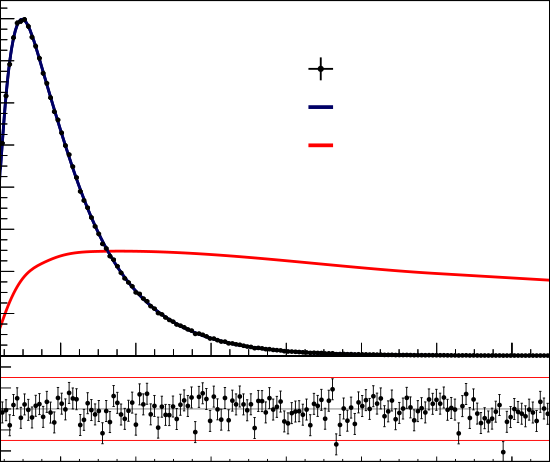
\includegraphics[width=0.9\textwidth]{BsDsK_TD/Time_Acceptance/time_Bs2DsK_BeautyTime_both_all_run1_Nominal}};
            \begin{scope}[x={(image.south east)},y={(image.north west)}]
                \foreach \x in {0, ..., 6}
                {
                    \tikzmath{\xpos = (\x / 6) * (0.931 - 0.111) + 0.111; \xtext = 2 * \x + 2;}
                    \node at (\xpos, -0.025) {\(\pgfmathprintnumber[fixed,precision=0,fixed zerofill=true]{\xtext}\)};
                }
                \foreach \y in {1, ..., 8}
                {
                    \tikzmath{\ypos = (\y / 8) * (0.963 - 0.230) + 0.230; \ytext = 2 * \y;}
                    \node[anchor=east] at (0.005, \ypos) {\(\pgfmathprintnumber[fixed,precision=0,fixed zerofill=true]{\ytext}\)};
                }
                \node[anchor=south] at (0.03, 1.) {\({\times \num{e3}}\)};
                \foreach \p in {0, ..., 4}
                {
                    \tikzmath{\ypos = (\p / 4) * (0.206 - 0.027) + 0.027; \ptext = (\p - 2) * 2;}
                    \node[anchor=east] at (0.005, \ypos) {\(\scriptstyle\pgfmathprintnumber[fixed,precision=0,fixed zerofill=true]{\ptext}\)};
                }
                % Legend
                {
                    \node[anchor=base west] at (0.61, 0.835) {\BsDsK~data};
                    \node[anchor=base west] at (0.61, 0.754) {Fit};
                    \node[anchor=base west] at (0.61, 0.673) {Acceptance};
                }
                \node[anchor=east] at (1.0, -0.09) {Decay time~\([\si{\ps}]\)};
                \node[rotate=90,anchor=east,inner xsep=0pt,outer xsep=0pt] at (-0.12, 1.0) {\({\text{Candidates}/(\SI{0.10}{\ps})}\)};
                \node[anchor=west] at (0.54, 0.93) {\Large\lhcb};
            \end{scope}
        \end{tikzpicture}
        \caption{Fit to simulated, untagged \BsDsK~sample.}
    \end{subfigure}
    \par\bigskip
    \begin{subfigure}{.8\textwidth} \centerfloat
        \begin{tikzpicture}
            \node[anchor=south west,inner sep=0] (image) at (0,0) {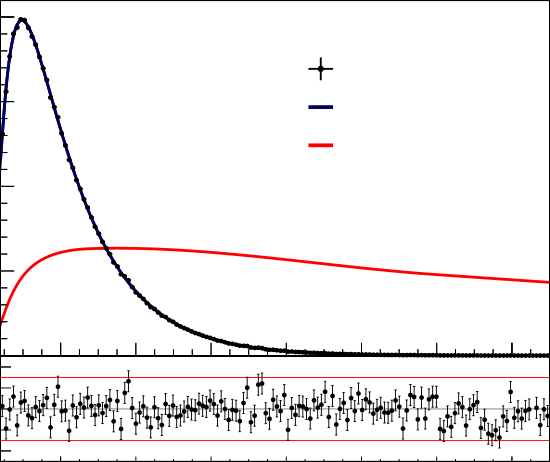
\includegraphics[width=0.9\textwidth]{BsDsK_TD/Time_Acceptance/time_Bs2DsPi_BeautyTime_both_all_run1_Nominal}};
            \begin{scope}[x={(image.south east)},y={(image.north west)}]
                \foreach \x in {0, ..., 6}
                {
                    \tikzmath{\xpos = (\x / 6) * (0.931 - 0.111) + 0.111; \xtext = 2 * \x + 2;}
                    \node at (\xpos, -0.025) {\(\pgfmathprintnumber[fixed,precision=0,fixed zerofill=true]{\xtext}\)};
                }
                \foreach \y in {1, ..., 4}
                {
                    \tikzmath{\ypos = (\y / 4) * (0.963 - 0.230) + 0.230; \ytext = 5 * \y;}
                    \node[anchor=east] at (0.005, \ypos) {\(\pgfmathprintnumber[fixed,precision=0,fixed zerofill=true]{\ytext}\)};
                }
                \node[anchor=south] at (0.03, 1.) {\({\times \num{e3}}\)};
                \foreach \p in {0, ..., 4}
                {
                    \tikzmath{\ypos = (\p / 4) * (0.206 - 0.027) + 0.027; \ptext = (\p - 2) * 2;}
                    \node[anchor=east] at (0.005, \ypos) {\(\scriptstyle\pgfmathprintnumber[fixed,precision=0,fixed zerofill=true]{\ptext}\)};
                }
                % Legend
                {
                    \node[anchor=base west] at (0.61, 0.835) {\BsDsPi~data};
                    \node[anchor=base west] at (0.61, 0.754) {Fit};
                    \node[anchor=base west] at (0.61, 0.673) {Acceptance};
                }
                \node[anchor=east] at (1.0, -0.09) {Decay time~\([\si{\ps}]\)};
                \node[rotate=90,anchor=east,inner xsep=0pt,outer xsep=0pt] at (-0.12, 1.0) {\({\text{Candidates}/(\SI{0.10}{\ps})}\)};
                \node[anchor=west] at (0.54, 0.93) {\Large\lhcb};
            \end{scope}
        \end{tikzpicture}
        \caption{Fit to simulated, untagged \BsDsPi~sample.}
    \end{subfigure}
    \caption{
        Decay-time fit to simulated samples (charge conjugation is implied). The fit is shown as a blue line, and the acceptance function is red.}
    \label{fig:BsDsK_TD_Acceptance_MC}
\end{figure}

\clearpage
\subsection{Fit parameters} \label{sec:BsDsK_TD_TimeFit_Formulas}

The final decay-time fit to the \BsDsK~candidates, to determine the \CP-violation observables, is an unbinned maximum likelihood fit.
It has six event observables: the weight from the multivariate fit, the decay time, the per-event decay-time error, the charge of the companion track (defining the charge of the \Bs~meson at the time of its decay), the combined tagging decision, and the predicted mistag probability~\(\eta\).

After taking into account all the effects, the fit parameters of the decay-time fits to the \BsDsPi~and \BsDsK~samples obtained from the multivariate fit are as listed in \cref{tab:BsDsK_TD_TimeFit_Parameters}.
The fit to the \BsDsPi~sample has seven free parameters: the six acceptance parameters~\(v_{1-6}\) and~\dms.
In the fit to the \BsDsK~sample, these acceptance parameters are then used (after correcting them as described in \cref{sec:BsDsK_TD_Acceptance}), while the \dms~value is taken from \hflav~\cite{HFLAV2016}.
Therefore the fit to the \BsDsK~sample has exactly five free parameters: the \CP-violation parameters~\Cpar, \Spar, \Sbpar, \Dpar, and \Dbpar.

Several other parameters are required as input to perform the fit.
Two of those, the decay-width parameters~\Gs and~\DGs, are taken directly from the 2016~\hflav results~\cite{HFLAV2016}.
In addition, two asymmetries~\AdetKPi and~\AprodBs, related to the \lhcb~kaon-pion detection asymmetry and the \(\Bsb\)--\(\Bs\)~production asymmetry, respectively, potentially distort the distributions.
The systematic uncertainty of each of these four values (taking into account the correlation between~\Gs and~\DGs) is determined using pseudoexperiments, as described in \cref{sec:BsDsK_TD_Syst}.
Other parameters used as input to the fit are discussed in the \lcnamecrefs{sec:BsDsK_TD_Res} above: the decay-time resolution calibration parameters~\(s_{0}\) and~\(s_{1}\), and the tagging parameters~\tagp0, \tagp1, \Dtagp0, \Dtagp1, and~\Detag, both for the OS and SS taggers, as reported in \cref{tab:BsDsK_TD_Tagging_Calibration}.
In the fit to the \BsDsK~sample, the first four of these tagging parameters have propagated directly into fit results using Gaussian constraints.
In the fit to the \BsDsPi~sample, they are instead fixed to the central values, as they were calibrated on that sample.
The tagging efficiency asymmetry is fixed to the value reported in \cref{sec:BsDsK_TD_Tagging}.

The detection asymmetry mentioned above is the difference in detection efficiency between a \(\Kp\pim\)~pair and a \(\Km\pip\)~pair, which enters in the \DsmKKPi~and \DsmPiPiPi~modes of the decay~\BsDsK, since these have a different number of pions and kaons in the final state (taking into account both the companion candidate and the \Dsm~decay products).
In the \DsmKPiPi~mode, the number of pions and kaons is equal, but the asymmetry may still show up because of the difference in kinematic distributions of the various particles.
Therefore, the central value is set to zero for that mode, although the uncertainty is used for determining systematic uncertainties (see \cref{sec:BsDsK_TD_Syst}).
In the fit to the self-tagging channel \BsDsPi, this asymmetry, as well as the \(\Bsb\)--\(\Bs\)~production asymmetry, are fixed to zero.
%
\begin{table}[htb] \centerfloat
    \caption{
        Parameters used in the two decay-time fits.
        The acceptance parameters~\(v_{1-6}\) are fixed to the values obtained in the fit to the \BsDsPi~sample, corrected as described in \cref{sec:BsDsK_TD_Acceptance}.
        Not listed are the decay-time resolution parameters (see \cref{sec:BsDsK_TD_Res}) and the flavour~tagging parameters (see \cref{sec:BsDsK_TD_Tagging}).}
    \label{tab:BsDsK_TD_TimeFit_Parameters}
    \begin{tabular}{lccl}
        \toprule
                            & \BsDsPi              & \BsDsK & Source \tabularnewline
        \midrule
        \Gs                 & \multicolumn{2}{c}{\SI{0.6643 +- 0.0020}{\per\ps}} & \hflav~\cite{HFLAV2016} \tabularnewline
        \rowcolor{tableshade}
        \DGs                & \multicolumn{2}{c}{\SI{0.083 +- 0.006}{\per\ps}} & \hflav~\cite{HFLAV2016} \tabularnewline
        \AdetKPi            & 0           & \SI{1.1 +- 2.7}{\percent} & \lhcb~measurement~\cite{LHCb-PAPER-2014-013} \tabularnewline
        \rowcolor{tableshade}
        \AprodBs            & 0           & \SI{1 +- 1}{\percent} & \lhcb~measurement~\cite{LHCb-PAPER-2014-042} \tabularnewline
        \midrule
        \dms                & \emph{Free} & \SI{17.757 +- 0.021}{\per\ps} & \hflav~\cite{HFLAV2016} \tabularnewline[.3ex]
        \rowcolor{tableshade}
        \(v_{1-6}\)         & \emph{Free} & Fixed       & \tabularnewline[.3ex]
        \Cpar               & \num{1}     & \emph{Free} & \tabularnewline[.3ex]
        \rowcolor{tableshade}
        \Spar               & \num{0}     & \emph{Free} & \tabularnewline[.3ex]
        \Sbpar              & \num{0}     & \emph{Free} & \tabularnewline[.3ex]
        \rowcolor{tableshade}
        \Dpar               & \num{0}     & \emph{Free} & \tabularnewline[.3ex]
        \Dbpar              & \num{0}     & \emph{Free} & \tabularnewline[.3ex]
        \bottomrule
    \end{tabular}
\end{table}

\clearpage
\subsection{Fit results} \label{sec:BsDsK_TD_TimeFit_Results}

The results of the decay-time fit to the \BsDsPi~sample yield the decay-time-acceptance parameters, and are presented in \cref{tab:BsDsK_TD_TimeFit_BsDsPi_Results,fig:BsDsK_TD_TimeFit_BsDsPi_Results}.
The fit results in a measurement of the \Bs~oscillation frequency~\({\dms = \SI{17.754 +- 0.013}{\per\pico\second}}\).
The quoted value is consistent with, but more precise than the current world-average result, although it should be noted that no systematic uncertainties are included.
The value is a by-product of the \CP-violation analysis and shows that a new measurement can be expected soon from~\lhcb.
The \({\Bs-\Bsb}\)~oscillations can be seen clearly in \cref{fig:BsDsK_TD_TimeFit_BsDsPi_Results_Tagged,fig:BsDsK_TD_TimeFit_BsDsPi_Asymmetry}, where the tagged mixed and unmixed events as well as the asymmetry between them are shown.
%
\begin{table}[htb] \centerfloat
    \caption{
        Fit results of the decay-time fit to the \BsDsPi~sample with weights from the multivariate fit applied.
        The third column lists the value of the acceptance parameters~\(v_{1-6}\) after applying the corrections in \cref{tab:BsDsK_TD_Acceptance_MC}, which are used in the decay-time fit to the \BsDsK~sample.}
    \label{tab:BsDsK_TD_TimeFit_BsDsPi_Results}
    \hspace*{-.75cm}
    \rowcolors{3}{tableshade}{}
    \begin{tabular}{l*{2}{S[table-format=1.3(3)]}*{5}{S[table-format=.3]}}
        \hiderowcolors \toprule
                    &                &                   & \multicolumn{5}{c}{Correlation} \tabularnewline
        \cmidrule(lr){4-8}
                    & {Fitted value} & {Corrected value} & {\(v_{2}\)} & {\(v_{3}\)} & {\(v_{4}\)} & {\(v_{5}\)} & {\(v_{6}\)} \tabularnewline
        \showrowcolors \midrule
        \(v_{1}\)   & 0.390 +- 0.014 & 0.366 +- 0.015    & 0.834       & 0.744       & 0.875       & 0.876       & 0.831 \tabularnewline
        \(v_{2}\)   & 0.596 +- 0.024 & 0.567 +- 0.025    &             & 0.542       & 0.850       & 0.788       & 0.777 \tabularnewline
        \(v_{3}\)   & 0.790 +- 0.031 & 0.779 +- 0.033    &             &             & 0.651       & 0.835       & 0.702 \tabularnewline
        \(v_{4}\)   & 1.014 +- 0.038 & 0.966 +- 0.040    &             &             &             & 0.826       & 0.875 \tabularnewline
        \(v_{5}\)   & 1.099 +- 0.036 & 1.070 +- 0.039    &             &             &             &             & 0.741 \tabularnewline
        \(v_{6}\)   & 1.189 +- 0.062 & 1.153 +- 0.066    &             &             &             &             & \tabularnewline
        \hiderowcolors \midrule
        \dms        & \multicolumn{2}{l}{\(\SI[parse-numbers=false]{(17.7535\,\pm\,0.0129)}{\per\ps}\)} \tabularnewline
        \bottomrule
    \end{tabular}
\end{table}
%
\begin{figure}[hp] \centerfloat
    \begin{tikzpicture}
        \node[anchor=south west,inner sep=0] (image) at (0,0) {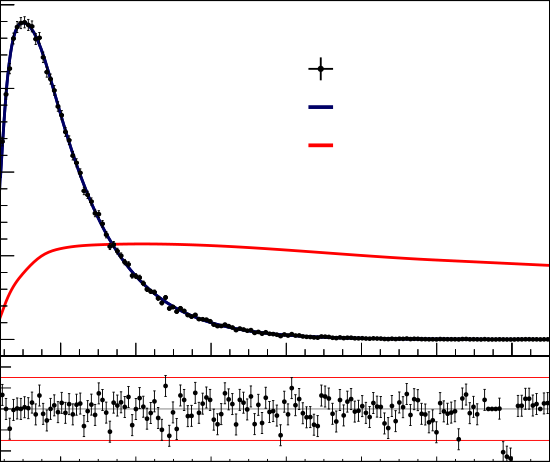
\includegraphics[width=0.8\textwidth]{BsDsK_TD/Time_Fits/time_Bs2DsPi_nominal_combopt}};
        \begin{scope}[x={(image.south east)},y={(image.north west)}]
            \foreach \x in {0, ..., 6}
            {
                \tikzmath{\xpos = (\x / 6) * (0.931 - 0.111) + 0.111; \xtext = 2 * \x + 2;}
                \node at (\xpos, -0.025) {\(\pgfmathprintnumber[fixed,precision=0,fixed zerofill=true]{\xtext}\)};
            }
            \foreach \y in {0, ..., 4}
            {
                \tikzmath{\ypos = (\y / 4) * (0.990 - 0.265) + 0.265; \ytext = \y;}
                \node[anchor=east] at (0.005, \ypos) {\(\pgfmathprintnumber[fixed,precision=0,fixed zerofill=true]{\ytext}\)};
            }
            \node[anchor=south] at (0.03, 1.) {\({\times \num{e3}}\)};
            \foreach \p in {0, ..., 4}
            {
                \tikzmath{\ypos = (\p / 4) * (0.206 - 0.027) + 0.027; \ptext = (\p - 2) * 2;}
                \node[anchor=east] at (0.005, \ypos) {\(\scriptstyle\pgfmathprintnumber[fixed,precision=0,fixed zerofill=true]{\ptext}\)};
            }
            % Legend
            {
                \node[anchor=base west] at (0.61, 0.835) {\BsDsPi~data};
                \node[anchor=base west] at (0.61, 0.754) {Fit};
                \node[anchor=base west] at (0.61, 0.673) {Acceptance};
            }
            \node[anchor=east] at (1.0, -0.09) {Decay time~\([\si{\ps}]\)};
            \node[rotate=90,anchor=east,inner xsep=0pt,outer xsep=0pt] at (-0.12, 1.0) {\({\text{Candidates}/(\SI{0.10}{\ps})}\)};
            \node[anchor=west] at (0.54, 0.93) {\Large\lhcb};
        \end{scope}
    \end{tikzpicture}
    \begin{tikzpicture}
        \node[anchor=south west,inner sep=0] (image) at (0,0) {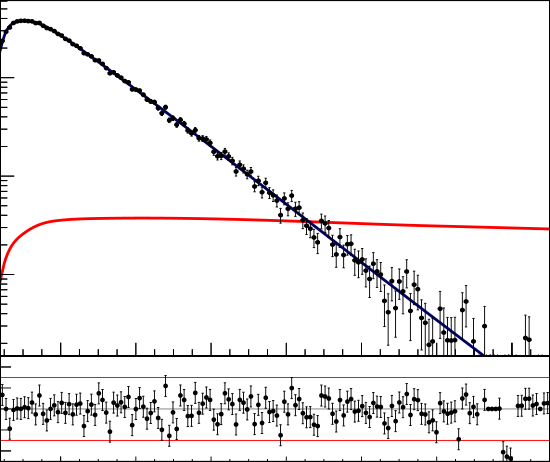
\includegraphics[width=0.8\textwidth]{BsDsK_TD/Time_Fits/time_Bs2DsPi_nominal_combopt_log}};
        \begin{scope}[x={(image.south east)},y={(image.north west)}]
            \foreach \x in {0, ..., 6}
            {
                \tikzmath{\xpos = (\x / 6) * (0.931 - 0.111) + 0.111; \xtext = 2 * \x + 2;}
                \node at (\xpos, -0.025) {\(\pgfmathprintnumber[fixed,precision=0,fixed zerofill=true]{\xtext}\)};
            }
            \node[anchor=base east] at (0.005, .394) {\num{10}};
            \node[anchor=base east] at (0.005, .608) {\num{e2}};
            \node[anchor=base east] at (0.005, .822) {\num{e3}};
            \foreach \p in {0, ..., 4}
            {
                \tikzmath{\ypos = (\p / 4) * (0.206 - 0.027) + 0.027; \ptext = (\p - 2) * 2;}
                \node[anchor=east] at (0.005, \ypos) {\(\scriptstyle\pgfmathprintnumber[fixed,precision=0,fixed zerofill=true]{\ptext}\)};
            }
            \node[anchor=east] at (1.0, -0.09) {Decay time~\([\si{\ps}]\)};
            \node[rotate=90,anchor=east,inner xsep=0pt,outer xsep=0pt] at (-0.12, 1.0) {\({\text{Candidates}/(\SI{0.10}{\ps})}\)};
            \node[anchor=west] at (0.54, 0.93) {\Large\lhcb};
        \end{scope}
    \end{tikzpicture}
    \caption{
        Results of the decay-time fit to the \BsDsPi~sample with weights from the multivariate fit applied.
        Top:~linear scale, bottom:~logarithmic scale.}
    \label{fig:BsDsK_TD_TimeFit_BsDsPi_Results}
\end{figure}
%
\begin{figure}[hp] \centerfloat
    \begin{tikzpicture}
        \node[anchor=south west,inner sep=0] (image) at (0,0) {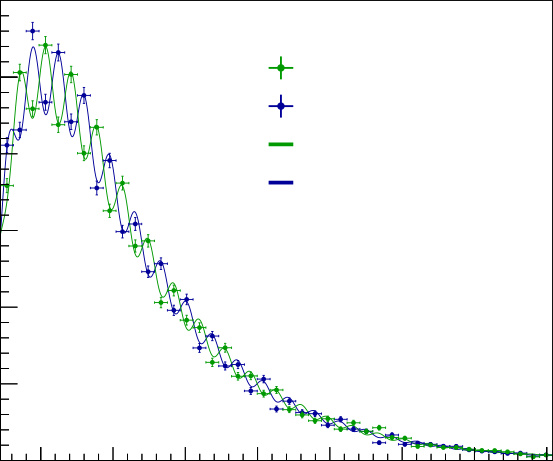
\includegraphics[width=0.8\textwidth]{BsDsK_TD/Time_Fits/time_Bs2DsPi_TaggedRates}};
        \begin{scope}[x={(image.south east)},y={(image.north west)}]
            \foreach \x in {1, ..., 8}
            {
                \tikzmath{\xpos = ((\x - 1) / 7) * (0.988 - 0.074) + 0.074;}
                \node at (\xpos, -0.025) {\(\pgfmathprintnumber[fixed,precision=0,fixed zerofill=true]{\x}\)};
            }
            \foreach \y in {0, ..., 5}
            {
                \tikzmath{\ypos = (\y / 6) * 0.997; \ytext = \y * 500;}
                \node[anchor=east] at (0.005, \ypos) {\(\pgfmathprintnumber[fixed,precision=0,fixed zerofill=true,1000 sep={}]{\ytext}\)};
            }
            % Legend
            {
                \node[anchor=base west] at (0.53, 0.835) {Unmixed~\BsDsPi~data};
                \node[anchor=base west] at (0.53, 0.754) {Mixed~\BsDsPi~data};
                \node[anchor=base west] at (0.53, 0.673) {Unmixed decay-time fit};
                \node[anchor=base west] at (0.53, 0.592) {Mixed decay-time fit};
            }
            \node[anchor=east] at (1.0, -0.09) {Decay time~\([\si{\ps}]\)};
            \node[rotate=90,anchor=east,inner xsep=0pt,outer xsep=0pt] at (-0.12, 1.0) {\({\text{Candidates}/(\SI{0.18}{\ps})}\)};
        \end{scope}
    \end{tikzpicture}
    \caption{
        Tagged events of the \BsDsPi~sample, showing both mixed and unmixed \Bs~candidates and the partial decay-time fit of each.}
    \label{fig:BsDsK_TD_TimeFit_BsDsPi_Results_Tagged}
\end{figure}
%
\begin{figure}[hp] \centerfloat
    \begin{tikzpicture}
        \node[anchor=south west,inner sep=0] (image) at (0,0) {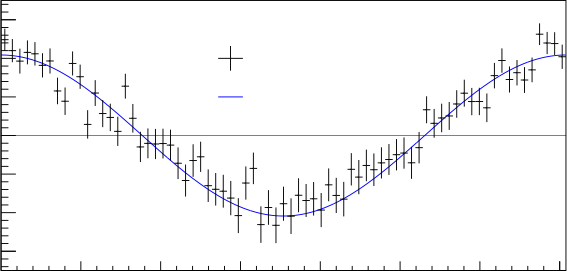
\includegraphics[width=0.8\textwidth]{figs/BsDsK_TD/Time_Fits/AsymmetryPlot_BsDsPi_3fb_Folded}};
        \begin{scope}[x={(image.south east)},y={(image.north west)}]
            \foreach \x in {0, ..., 7}
            {
                \tikzmath{\xtext = \x / 20; \xcoord = \x * .141;}
                \node at (\xcoord, -0.040) {\(\pgfmathprintnumber[fixed,precision=2,fixed zerofill=true]{\xtext}\)};
            }
            \foreach \y in {0, ..., 6}
            {
                \tikzmath{\ytext = \y / 10 - 0.3; \ycoord = \y * .142 + .074;}
                \node[anchor=east] at (0.005, \ycoord) {\(\pgfmathprintnumber[fixed,precision=1,fixed zerofill=true]{\ytext}\)};
            }
            % Legend
            {
                \node[anchor=base west] at (0.42, 0.765) {\BsDsPi~data};
                \node[anchor=base west] at (0.42, 0.623) {\({\cos(\dms t)}\)};
            }
            \node[anchor=east] at (1.0, -0.15) {\(t(\BsDsPi)\) modulo~\((2\pi/\dms)\)~[\si{\pico\second}]};
            \node[rotate=90,anchor=east,inner xsep=0pt,outer xsep=0pt] at (-0.10, 1.0) {Asymmetry};
        \end{scope}
    \end{tikzpicture}
    \caption{
        Distribution of the time-dependent \BsDsPi~flavour asymmetry modulo~\({2\pi/\dms}\), using the value of~\dms reported in \cref{tab:BsDsK_TD_TimeFit_BsDsPi_Results}.
        Overlaid is the function~\({A \cos(\dms t)}\) to which the asymmetry should correspond, with the amplitude~\(A\) fitted to match the data.
        The line corresponding to an asymmetry of zero is also shown.}
    \label{fig:BsDsK_TD_TimeFit_BsDsPi_Asymmetry}
\end{figure}

\clearpage
Using the corrected acceptance parameters as reported in \cref{tab:BsDsK_TD_TimeFit_BsDsPi_Results}, the decay-time fit is also performed on the \BsDsK~sample.
This yields the five \CP-violation parameters,~\Cpar, \Spar, \Sbpar, \Dpar, and~\Dbpar, as defined in \cref{sec:theory_CPV}. The values and correlations of these parameters are presented in \Cref{tab:BsDsK_TD_TimeFit_BsDsK_Results}, and the fit is shown in \cref{fig:BsDsK_TD_TimeFit_BsDsK_Results}.
%
\begin{table}[htb] \centerfloat
    \caption{
        Results of the decay-time fit to the \BsDsK~sample with weights from the multivariate fit applied.}
    \label{tab:BsDsK_TD_TimeFit_BsDsK_Results}
    \rowcolors{3}{tableshade}{}
    \begin{tabular}{lS[table-format=+.3(3)]*{4}{S[table-format=+.3]}}
        \hiderowcolors \toprule
                    &                  & \multicolumn{4}{c}{Correlation} \tabularnewline
        \cmidrule(lr){3-6}
        {Parameter} & {Fitted value}   & {\Spar} & {\Sbpar} & {\Dpar}  & {\Dbpar} \tabularnewline
        \showrowcolors \midrule
        \Cpar       &  0.730 +- 0.142  & 0.008   & -0.057   &  0.092   &  0.078 \tabularnewline[.3ex]
        \Spar       & -0.519 +- 0.202  &         &  0.001   & -0.083   & -0.042 \tabularnewline[.3ex]
        \Sbpar      & -0.489 +- 0.196  &         &          & -0.004   & -0.003 \tabularnewline[.3ex]
        \Dpar       &  0.387 +- 0.277  &         &          &          &  0.513 \tabularnewline[.3ex]
        \Dbpar      &  0.308 +- 0.275  &         &          &          &        \tabularnewline[.3ex]
        \bottomrule
    \end{tabular}
\end{table}
%
\begin{figure}[hp] \centerfloat
    \begin{tikzpicture}
        \node[anchor=south west,inner sep=0] (image) at (0,0) {\includegraphics[width=0.8\textwidth]{BsDsK_TD/Time_Fits/time_Bs2DsK}};
        \begin{scope}[x={(image.south east)},y={(image.north west)}]
            \foreach \x in {0, ..., 6}
            {
                \tikzmath{\xpos = (\x / 6) * (0.931 - 0.111) + 0.111; \xtext = 2 * \x + 2;}
                \node at (\xpos, -0.025) {\(\pgfmathprintnumber[fixed,precision=0,fixed zerofill=true]{\xtext}\)};
            }
            \foreach \y in {0, ..., 5}
            {
                \tikzmath{\ypos = (\y / 5) * (0.906 - 0.268) + 0.268; \ytext = 50 * \y;}
                \node[anchor=east] at (0.005, \ypos) {\(\pgfmathprintnumber[fixed,precision=0,fixed zerofill=true]{\ytext}\)};
            }
            \foreach \p in {0, ..., 4}
            {
                \tikzmath{\ypos = (\p / 4) * (0.206 - 0.027) + 0.027; \ptext = (\p - 2) * 2;}
                \node[anchor=east] at (0.005, \ypos) {\(\scriptstyle\pgfmathprintnumber[fixed,precision=0,fixed zerofill=true]{\ptext}\)};
            }
            % Legend
            {
                \node[anchor=base west] at (0.61, 0.835) {\BsDsK~data};
                \node[anchor=base west] at (0.61, 0.754) {Fit};
            }
            \node[anchor=east] at (1.0, -0.09) {Decay time~\([\si{\ps}]\)};
            \node[rotate=90,anchor=east,inner xsep=0pt,outer xsep=0pt] at (-0.12, 1.0) {\({\text{Candidates}/(\SI{0.10}{\ps})}\)};
            \node[anchor=west] at (0.54, 0.93) {\Large\lhcb};
        \end{scope}
    \end{tikzpicture}
    \begin{tikzpicture}
        \node[anchor=south west,inner sep=0] (image) at (0,0) {\includegraphics[width=0.8\textwidth]{BsDsK_TD/Time_Fits/time_Bs2DsK_log}};
        \begin{scope}[x={(image.south east)},y={(image.north west)}]
            \foreach \x in {0, ..., 6}
            {
                \tikzmath{\xpos = (\x / 6) * (0.931 - 0.111) + 0.111; \xtext = 2 * \x + 2;}
                \node at (\xpos, -0.025) {\(\pgfmathprintnumber[fixed,precision=0,fixed zerofill=true]{\xtext}\)};
            }
            \node[anchor=base east] at (0.005, .474) {\num{10}};
            \node[anchor=base east] at (0.005, .787) {\num{e2}};
            \foreach \p in {0, ..., 4}
            {
                \tikzmath{\ypos = (\p / 4) * (0.206 - 0.027) + 0.027; \ptext = (\p - 2) * 2;}
                \node[anchor=east] at (0.005, \ypos) {\(\scriptstyle\pgfmathprintnumber[fixed,precision=0,fixed zerofill=true]{\ptext}\)};
            }
            \node[anchor=east] at (1.0, -0.09) {Decay time~\([\si{\ps}]\)};
            \node[rotate=90,anchor=east,inner xsep=0pt,outer xsep=0pt] at (-0.12, 1.0) {\({\text{Candidates}/(\SI{0.10}{\ps})}\)};
            \node[anchor=west] at (0.54, 0.93) {\Large\lhcb};
        \end{scope}
    \end{tikzpicture}
    \caption{
        Results of the decay-time fit to the \BsDsK~sample with weights from the multivariate fit applied.
        Top:~linear scale, bottom:~logarithmic scale.}
    \label{fig:BsDsK_TD_TimeFit_BsDsK_Results}
\end{figure}
%
\begin{figure}[hp] \centerfloat
    \begin{subfigure}{\textwidth}
        \begin{tikzpicture}
            \node[anchor=south west,inner sep=0] (image) at (0,0) {\includegraphics[width=0.8\textwidth]{figs/BsDsK_TD/Time_Fits/asymmetry_Bs2Ds+K-_folded}};
            \begin{scope}[x={(image.south east)},y={(image.north west)}]
                \foreach \x in {0, ..., 3}
                {
                    \tikzmath{\xtext = \x / 10; \xcoord = \x * .282;}
                    \node at (\xcoord, -0.040) {\(\pgfmathprintnumber[fixed,precision=1,fixed zerofill=true]{\xtext}\)};
                }
                \foreach \y in {0, ..., 4}
                {
                    \tikzmath{\ytext = \y / 5 - 0.4; \ycoord = \y * .199 + .102;}
                    \node[anchor=east] at (0.005, \ycoord) {\(\pgfmathprintnumber[fixed,precision=1,fixed zerofill=true]{\ytext}\)};
                }
                \node[anchor=east] at (1.0, -0.12) {\(t(\BsDspKm)\)~modulo~\((2\pi/\dms)\)~[\si{\pico\second}]};
                \node[rotate=90,anchor=east,inner xsep=0pt,outer xsep=0pt] at (-0.12, 1.0) {\(A_{\text{mix}} (\DspKm)\)};
                \node[anchor=base east] at (0.94, 0.823) {\Huge\lhcb};
            \end{scope}
        \end{tikzpicture}
        \caption{Asymmetry for the final state~\DspKm.}
    \end{subfigure}
    \\[4ex]
    \begin{subfigure}{\textwidth}
        \begin{tikzpicture}
            \node[anchor=south west,inner sep=0] (image) at (0,0) {\includegraphics[width=0.8\textwidth]{figs/BsDsK_TD/Time_Fits/asymmetry_Bs2Ds-K+_folded}};
            \begin{scope}[x={(image.south east)},y={(image.north west)}]
                \foreach \x in {0, ..., 3}
                {
                    \tikzmath{\xtext = \x / 10; \xcoord = \x * .282;}
                    \node at (\xcoord, -0.040) {\(\pgfmathprintnumber[fixed,precision=1,fixed zerofill=true]{\xtext}\)};
                }
                \foreach \y in {0, ..., 4}
                {
                    \tikzmath{\ytext = \y / 5 - 0.4; \ycoord = \y * .199 + .102;}
                    \node[anchor=east] at (0.005, \ycoord) {\(\pgfmathprintnumber[fixed,precision=1,fixed zerofill=true]{\ytext}\)};
                }
                \node[anchor=east] at (1.0, -0.12) {\(t(\BsDsmKp)\)~modulo~\((2\pi/\dms)\)~[\si{\pico\second}]};
                \node[rotate=90,anchor=east,inner xsep=0pt,outer xsep=0pt] at (-0.12, 1.0) {\(A_{\text{mix}} (\DsmKp)\)};
                \node[anchor=base east] at (0.94, 0.823) {\Huge\lhcb};
            \end{scope}
        \end{tikzpicture}
        \caption{Asymmetry for the final state~\DsmKp.}
    \end{subfigure}
    \caption{
        \CP~asymmetry of the \BsDsK~candidates, separately for each final state.
        The asymmetries are enhanced by being folded into one mixing period.
        The horizontal lines indicate an asymmetry of zero.}
    \label{fig:BsDsK_TD_DsK_Asymmetry}
\end{figure}

\clearpage
\section{Systematic effects} \label{sec:BsDsK_TD_Syst}

\subsection{Systematic uncertainties}

Several systematic effects can bias the fit results, and must be accounted for by evaluating their respective size and assigning a systematic error.
These effects are the following:
%
\begin{itemize}
    \item The detection asymmetry,~\AdetKPi;
    \item The \Bs~oscillation frequency,~\dms;
    \item The tagging efficiency asymmetry,~\Detag, both for OS~and SS~tagging;
    \item Possible correlations between the three multivariate fit variables and the decay time;
    \item The combination of decay-time resolution and flavour tagging;
    \item The combination of decay-time acceptance and the values of~\Gs and~\DGs;
    \item The sensitivity of a closure test using a simulated sample, quantifying the modelling of the decay-time acceptance.
\end{itemize}
%
All systematic uncertainties, with the exception of the closure test, are evaluated using pseudoexperiments.
The systematic uncertainties on the \CP-violation parameters are calculated from these pseudoexperiments by taking into account both the bias and the spread of the values,
%
\begin{equation} \label{eqn:BsDsK_TD_Syst_Pseudoexperiments}
    \sigma_{p,\text{syst}} = \sqrt{\mean{\mu_{p}}^{2} + \sigma_{p}^{2}} \rlap{,}
\end{equation}
%
where \({p \in \{ \Cpar, \Spar, \Sbpar, \Dpar, \Dbpar \}}\)~runs over the observables, \(\mean{\mu_{p}}\)~is the deviation in central value of~\(p\), and \(\sigma_{p}\)~is the total width of the distribution of~\(p\) from the combination of the pseudoexperiments.

For each of~\AdetKPi, \dms,~and both~\Detag, two sets of pseudoexperiments are performed: one where the value under investigation is increased by its uncertainty, and one where it is decreased.
To obtain~\(\mean{\mu_{p}}\), the deviations of the two sets of experiments are averaged.
In addition, the correlations between the observables are taken into account using the covariances of the pseudoexperiment data sets.

To determine the systematic uncertainty arising from correlations between~\({m(\Bs)}\), \({m(\Dsm)}\), companion~\(\dllkpi\), and decay time, samples of pseudoexperiments are generated including correlations among these four variables.
These samples include signal, physics backgrounds, and combinatorial, with the yield of each component sampled from a Poisson distribution with the fitted yields (\cref{tab:BsDsK_TD_DsK_MDFit_Results}) as parameters.
A decay-time fit is performed on each sample, and compared to a fit on only the signal and combinatorial components of the same sample.
The resulting systematic errors are calculated using \cref{eqn:BsDsK_TD_Syst_Pseudoexperiments} and quoted in \cref{tab:BsDsK_TD_Syst}.

The systematic uncertainty on the combination of decay-time resolution and tagging is assessed by performing decay-time fits on \BsDsK~pseudoexperiments, using the two different decay-time resolution models presented in \cref{eqn:BsDsK_TD_Res_Syst} and the corresponding tagging parameters from \cref{tab:BsDsK_TD_Tagging_ResSyst}.
\Cref{eqn:BsDsK_TD_Syst_Pseudoexperiments} is again used to calculate the corresponding systematic uncertainties.

The decay-width parameters~\Gs and~\DGs and the spline parameters~\(v_{1-6}\) together define the exponential shape in the \Bs~decay-time distribution.
Because of that, they are inherently correlated, and an assessment of their contribution to the systematic error must take this correlation into account.
This is done by generating new sets of values for these parameters, sampling them from multi-dimensional Gaussian distributions.
The sampling takes into account the correlation between~\Gs and~\DGs~\cite{HFLAV2016}.
This is done for two independent sets of variables: on the six spline ratio parameters (\cref{tab:BsDsK_TD_Acceptance_MC}), and on the eight values~\Gs, \DGs, and~\(v_{1-6}\).

Finally, a closure test is performed.
This test validates the fit procedure by applying it to a \BsDsK~sample, simulated with \CP~violation.
The decay-time acceptance parameters are taken from a simulated \BsDsK~sample without \CP~violation, hence the closure test also assesses the applicability of the decay-time acceptance from a sample without \CP~violation to one with.
The results of the fit to the simulated sample, are presented in \cref{tab:BsDsK_TD_Syst_ClosureTest}.
The fit shows good agreement, indicating the efficacy of the decay-time fit.
The uncertainties on the fitted \CP-violation parameters are only due to the fit procedure, and are included as a systematic uncertainty.
%
\begin{table}[p] \centerfloat
    \caption{
        Results of the closure test.
        Listed are the values with which the simulated sample was generated, the results of the decay-time fit, and the difference with the nominal fit (\cref{tab:BsDsK_TD_TimeFit_BsDsK_Results}).}
    \label{tab:BsDsK_TD_Syst_ClosureTest}
    \rowcolors{3}{}{tableshade}
    \begin{tabular}{lS[table-format=+.5]*{2}{S[table-format=+.3(3)]}}
        \toprule
        Parameter & {Generated} & {Fitted}        & {Difference}     \tabularnewline
                  &             &                 & {w.r.t. nominal} \tabularnewline
        \midrule
        \Cpar     &  0.75917    &  0.769 +- 0.017 &  0.010 +- 0.017  \tabularnewline[.3ex]
        \Spar     & -0.56995    & -0.579 +- 0.024 &  0.009 +- 0.024  \tabularnewline[.3ex]
        \Sbpar    & -0.64309    & -0.653 +- 0.023 & -0.010 +- 0.023  \tabularnewline[.3ex]
        \Dpar     &  0.31436    &  0.301 +- 0.051 & -0.013 +- 0.051  \tabularnewline[.3ex]
        \Dbpar    &  0.10046    &  0.059 +- 0.050 & -0.041 +- 0.050  \tabularnewline[.3ex]
        \bottomrule
    \end{tabular}
\end{table}

\Cref{tab:BsDsK_TD_Syst} lists for each observable the values of each systematic uncertainty, as well as their total when added in quadrature.
It also shows the final systematic correlations between the observables.
%
\begin{table}[hp] \centerfloat
    \caption{
        Systematic uncertainties on the \CP-violation parameters, and correlations between the systematic effects.
        The largest contributions are underlined.}
    \label{tab:BsDsK_TD_Syst}
    \begin{tabular}{l*{5}{S[table-format=.3]}}
        \toprule
        Fitted value                 & \Cpar   & \Spar   & \Sbpar  & \Dpar   & \Dbpar  \tabularnewline
        \midrule
        Detection asymmetry          & 0.003 & 0.004 & 0.004 & \underline{0.078} & \underline{0.080} \tabularnewline
        \rowcolor{tableshade}
        \dms                         & 0.016 & \underline{0.040} & \underline{0.039} & 0.006 & 0.006 \tabularnewline
        Tagging efficiency asymmetry & 0.003 & 0.004 & 0.004 & 0.000 & 0.000 \tabularnewline
        \rowcolor{tableshade}
        Correlations                 & \underline{0.028} & \underline{0.040} & \underline{0.035} & \underline{0.105} & \underline{0.105} \tabularnewline
        Resolution and tagging       & \underline{0.026} & \underline{0.032} & \underline{0.035} & 0.006 & 0.006 \tabularnewline
        \rowcolor{tableshade}
        Acceptance,~\Gs, and~\DGs    & 0.001 & 0.002 & 0.002 & 0.058 & 0.055 \tabularnewline
        Closure test                 & 0.017 & 0.024 & 0.023 & 0.051 & 0.050 \tabularnewline
        \midrule
        Total                        & 0.045 & 0.071 & 0.069 & 0.152 & 0.151 \tabularnewline
        \midrule
        Correlations                 &       &       &       &       & \tabularnewline
        \midrule
        \quad \Spar                  &  0.03 &       &       &       & \tabularnewline[.3ex]
        \rowcolor{tableshade}
        \quad \Sbpar                 & -0.01 & 0.01  &       &       & \tabularnewline[.3ex]
        \quad \Dpar                  &  0.05 & 0.02  & 0.02  &       & \tabularnewline[.3ex]
        \rowcolor{tableshade}
        \quad \Dbpar                 &  0.03 & 0.03  & 0.03  & 0.42  & \tabularnewline[.3ex]
        \bottomrule
    \end{tabular}
\end{table}

\clearpage
\subsection{Cross checks} \label{sec:BsDsK_TD_CrossChecks}

A number of cross checks are performed on various parts of the analysis.
These do not directly contribute to the systematic uncertainty, but are interesting as they verify the stability of the fits and methods.
The following cross checks are considered:
%
\begin{description}
    \item[Pseudoexperiments to assess the fit uncertainties.]
        For both the \BsDsPi~sample and the \BsDsK~sample, pseudoexperiments are generated on the event yields from the multivariate fit, as well as on each of the free parameters of the time fits.
        Each resulting pull distribution is found to be unbiased and its respective width compatible with~\num{1}, indicating the fits return reliable uncertainties.
    \item[Validation of the effect of the production asymmetry.]
        The production asymmetry has an intrinsic uncertainty, and its effect on the fit results is determined by generating pseudoexperiments from the fit results with different values for the production asymmetry.
        These pseudoexperiments are generated with~\SI{1 +- 3}{\percent} and~\SI{3 +- 3}{\percent} for \bquark~mesons and \Lb~baryons, respectively, and no change in decay-time fit results is observed.
    \item[Decay-time fits on partial data.]
        The data samples are split in three ways: \lhcb~magnet polarity, BDT~response, and \Bs~momentum split at~\SI{120}{\GeVc}.
        Each split yields consistent results.
    \item[Repeating the decay-time fits with different background yields.]
        The background yields are doubled and halved, respectively, and decay-time fit results remain invariant under each of these operations.
    \item[Repeating the decay-time fits with different signal shape parameters.]
        The signal shape parameters, for each \Dspm~mode, are shifted up and down with their error, respectively.
        The change in fit results is again negligible.
    \item[Using a different number of spline knots.]
        Adding one or two additional spline knots to the functional form of the decay-time acceptance does not change any of the fit results significantly.
\end{description}

\clearpage
\section{Results} \label{sec:BsDsK_TD_Results}

Taking into account the total systematic uncertainties, the \CP-violation parameters are
%
\begin{align} \label{eqn:BsDsK_TD_Results}
    \Cpar  &= \n0.73\,\pm\,0.14\,\pm\,0.05 \rlap{,} \\
    \Spar  &=  -0.52\,\pm\,0.20\,\pm\,0.07 \rlap{,} \\
    \Sbpar &=  -0.49\,\pm\,0.20\,\pm\,0.07 \rlap{,} \\
    \Dpar  &= \n0.39\,\pm\,0.28\,\pm\,0.15 \rlap{,} \\
    \Dbpar &= \n0.31\,\pm\,0.28\,\pm\,0.15 \rlap{,}
\end{align}
%
where the first uncertainties are statistical and the second systematic.

